%%%%%%%%%%%%%%%%%%%%%%%%%%%%%%%%%%%%%%%%%
% Masters/Doctoral Thesis 
% LaTeX Template
% Version 2.5 (27/8/17)
%
% This template was downloaded from:
% http://www.LaTeXTemplates.com
%
% Version 2.x major modifications by:
% Vel (vel@latextemplates.com)
%
% This template is based on a template by:
% Steve Gunn (http://users.ecs.soton.ac.uk/srg/softwaretools/document/templates/)
% Sunil Patel (http://www.sunilpatel.co.uk/thesis-template/)
%
% Template license:
% CC BY-NC-SA 3.0 (http://creativecommons.org/licenses/by-nc-sa/3.0/)
%
%%%%%%%%%%%%%%%%%%%%%%%%%%%%%%%%%%%%%%%%%

%----------------------------------------------------------------------------------------
%	PACKAGES AND OTHER DOCUMENT CONFIGURATIONS
%----------------------------------------------------------------------------------------

\documentclass[
11pt, % The default document font size, options: 10pt, 11pt, 12pt
%oneside, % Two side (alternating margins) for binding by default, uncomment to switch to one side
english, % ngerman for German
singlespacing, % Single line spacing, alternatives: onehalfspacing or doublespacing
%draft, % Uncomment to enable draft mode (no pictures, no links, overfull hboxes indicated)
%nolistspacing, % If the document is onehalfspacing or doublespacing, uncomment this to set spacing in lists to single
%liststotoc, % Uncomment to add the list of figures/tables/etc to the table of contents
%toctotoc, % Uncomment to add the main table of contents to the table of contents
%parskip, % Uncomment to add space between paragraphs
%nohyperref, % Uncomment to not load the hyperref package
headsepline, % Uncomment to get a line under the header
%chapterinoneline, % Uncomment to place the chapter title next to the number on one line
%consistentlayout, % Uncomment to change the layout of the declaration, abstract and acknowledgements pages to match the default layout
]{DoctoralThesis} % The class file specifying the document structure

\usepackage[utf8]{inputenc} % Required for inputting international characters
%\usepackage[cp1252]{inputenc}
\usepackage[T1]{fontenc} % Output font encoding for international characters

\usepackage{mathpazo} % Use the Palatino font by default

\usepackage[backend=bibtex,style=ieee,natbib=true]{biblatex} % Use the bibtex backend with the authoryear citation style (which resembles APA)

\addbibresource{References.bib} % The filename of the bibliography

\usepackage[autostyle=true]{csquotes} % Required to generate language-dependent quotes in the bibliography

\usepackage{ dsfont }
\usepackage{ amssymb }
\usepackage{braket,amsmath}
\usepackage{bm}
\usepackage{gensymb}
\graphicspath{{C:/Users/Steffi/Dropbox/THESIS/thesis/Figures/}}


%----------------------------------------------------------------------------------------
%	COMMANDS
%----------------------------------------------------------------------------------------

%\newcommand{\ket}[1]{|#1\rangle}
%\newcommand{\bra}[1]{\langle #1|}
%\newcommand{\braket}[2]{j(t)|e}
\newcommand{\mb}[1]{\boldsymbol{#1}}


%----------------------------------------------------------------------------------------
%	MARGIN SETTINGS
%----------------------------------------------------------------------------------------

\geometry{
	paper=a4paper, % Change to letterpaper for US letter
	inner=2.5cm, % Inner margin
	outer=3.8cm, % Outer margin
	bindingoffset=.5cm, % Binding offset
	top=1.5cm, % Top margin
	bottom=1.5cm, % Bottom margin
	%showframe, % Uncomment to show how the type block is set on the page
}

%----------------------------------------------------------------------------------------
%	THESIS INFORMATION
%----------------------------------------------------------------------------------------

\thesistitle{Advances in donor-based spin qubits in silicon: spin relaxation and flip-flop qubits} % Your thesis title, this is used in the title and abstract, print it elsewhere with \ttitle
\supervisor{Prof. Andrea \textsc{Morello}} % Your supervisor's name, this is used in the title page, print it elsewhere with \supname
%\supervisor{Dr. Vivien \textsc{Schmitt}}
\examiner{} % Your examiner's name, this is not currently used anywhere in the template, print it elsewhere with \examname
\ddegree{Doctor of Philosophy} % Your degree name, this is used in the title page and abstract, print it elsewhere with \degreename
\author{Stefanie \textsc{Tenberg}} % Your name, this is used in the title page and abstract, print it elsewhere with \authorname
\addresses{} % Your address, this is not currently used anywhere in the template, print it elsewhere with \addressname

\subject{Electrical Engineering} % Your subject area, this is not currently used anywhere in the template, print it elsewhere with \subjectname
\keywords{Quantum computation, silicon, phosphorus} % Keywords for your thesis, this is not currently used anywhere in the template, print it elsewhere with \keywordnames
\university{\href{http://www.unsw.edu.au}{Univerty of New South Wales}} % Your university's name and URL, this is used in the title page and abstract, print it elsewhere with \univname
\department{\href{http://www.engineering.unsw.edu.au/electrical-engineering/}{School of Electrical Engineering}} % Your department's name and URL, this is used in the title page and abstract, print it elsewhere with \deptname
\group{\href{http://researchgroup.university.com}{Fundamental Quantum T}} % Your research group's name and URL, this is used in the title page, print it elsewhere with \groupname
\faculty{\href{http://www.cqc2t.org/}{Center for Quantum Computation and Communication Technology}} % Your faculty's name and URL, this is used in the title page and abstract, print it elsewhere with \facname

\AtBeginDocument{
\hypersetup{pdftitle=\ttitle} % Set the PDF's title to your title
\hypersetup{pdfauthor=\authorname} % Set the PDF's author to your name
\hypersetup{pdfkeywords=\keywordnames} % Set the PDF's keywords to your keywords
}



\begin{document}

\frontmatter % Use roman page numbering style (i, ii, iii, iv...) for the pre-content pages

\pagestyle{plain} % Default to the plain heading style until the thesis style is called for the body content

%----------------------------------------------------------------------------------------
%	TITLE PAGE
%----------------------------------------------------------------------------------------

\begin{titlepage}
\begin{center}

\vspace*{.06\textheight}
{\scshape\LARGE \univname\par}\vspace{1.5cm} % University name
\textsc{\Large Doctoral Thesis}\\[0.5cm] % Thesis type

\HRule \\[0.4cm] % Horizontal line
{\huge \bfseries \ttitle\par}\vspace{0.4cm} % Thesis title
\HRule \\[1.5cm] % Horizontal line
 
\begin{minipage}[t]{0.4\textwidth}
\begin{flushleft} \large
\emph{Author:}\\
{\authorname} % Author name - remove the \href bracket to remove the link
\end{flushleft}
\end{minipage}
\begin{minipage}[t]{0.4\textwidth}
\begin{flushright} \large
\emph{Supervisor:} \\
{\supname} % Supervisor name - remove the \href bracket to remove the link  
\emph{Co-Supervisor:}\\
%{\cosupname}
\end{flushright}
\end{minipage}\\[3cm]
 
\vfill

\large \textit{A thesis submitted in fulfillment of the requirements\\ for the degree of \degreename}\\[0.3cm] % University requirement text
\textit{in the}\\[0.4cm]
\groupname\\\deptname\\[2cm] % Research group name and department name
 
\vfill

{\large \today}\\[4cm] % Date
%\includegraphics{Logo} % University/department logo - uncomment to place it
 
\vfill
\end{center}
\end{titlepage}

%----------------------------------------------------------------------------------------
%	DECLARATION PAGE
%----------------------------------------------------------------------------------------

\begin{declaration}
\addchaptertocentry{\authorshipname} % Add the declaration to the table of contents
\noindent I, \authorname, declare that this thesis titled, \enquote{\ttitle} and the work presented in it are my own. I confirm that:

\begin{itemize} 
\item This work was done wholly or mainly while in candidature for a research degree at this University.
\item Where any part of this thesis has previously been submitted for a degree or any other qualification at this University or any other institution, this has been clearly stated.
\item Where I have consulted the published work of others, this is always clearly attributed.
\item Where I have quoted from the work of others, the source is always given. With the exception of such quotations, this thesis is entirely my own work.
\item I have acknowledged all main sources of help.
\item Where the thesis is based on work done by myself jointly with others, I have made clear exactly what was done by others and what I have contributed myself.\\
\end{itemize}
 
\noindent Signed:\\
\rule[0.5em]{25em}{0.5pt} % This prints a line for the signature
 
\noindent Date:\\
\rule[0.5em]{25em}{0.5pt} % This prints a line to write the date
\end{declaration}

\cleardoublepage

%----------------------------------------------------------------------------------------
%	QUOTATION PAGE
%----------------------------------------------------------------------------------------

\vspace*{0.2\textheight}

\noindent\enquote{\itshape Nature isn't classical, […], and if you want to make a simulation of nature, you'd better make it quantum mechanical, and […] it's a wonderful problem, because it doesn't look so easy.}\bigbreak

\hfill Richard Feynman, 1982

\noindent\enquote{\itshape Those who dance are considered insane by those who can't hear the music.}\bigbreak

\hfill Friedrich Nietzsche

%----------------------------------------------------------------------------------------
%	ABSTRACT PAGE
%----------------------------------------------------------------------------------------

\begin{abstract}
\addchaptertocentry{\abstractname} % Add the abstract to the table of contents
The Thesis Abstract is written here (and usually kept to just this page). The page is kept centered vertically so can expand into the blank space above the title too\ldots
\end{abstract}

%----------------------------------------------------------------------------------------
%	ACKNOWLEDGEMENTS
%----------------------------------------------------------------------------------------

\begin{acknowledgements}
\addchaptertocentry{\acknowledgementname} % Add the acknowledgements to the table of contents
The acknowledgments and the people to thank go here, don't forget to include your project advisor\ldots
\end{acknowledgements}

%----------------------------------------------------------------------------------------
%	LIST OF CONTENTS/FIGURES/TABLES PAGES
%----------------------------------------------------------------------------------------

\tableofcontents % Prints the main table of contents

\listoffigures % Prints the list of figures

\listoftables % Prints the list of tables

%----------------------------------------------------------------------------------------
%	ABBREVIATIONS
%----------------------------------------------------------------------------------------

\begin{abbreviations}{ll} % Include a list of abbreviations (a table of two columns)

\textbf{LAH} & \textbf{L}ist \textbf{A}bbreviations \textbf{H}ere\\
\textbf{WSF} & \textbf{W}hat (it) \textbf{S}tands \textbf{F}or\\

\end{abbreviations}

%----------------------------------------------------------------------------------------
%	PHYSICAL CONSTANTS/OTHER DEFINITIONS
%----------------------------------------------------------------------------------------

\begin{constants}{lr@{${}={}$}l} % The list of physical constants is a three column table

% The \SI{}{} command is provided by the siunitx package, see its documentation for instructions on how to use it

Speed of Light & $c_{0}$ & \SI{2.99792458e8}{\meter\per\second} (exact)\\
%Constant Name & $Symbol$ & $Constant Value$ with units\\

\end{constants}

%----------------------------------------------------------------------------------------
%	SYMBOLS
%----------------------------------------------------------------------------------------

\begin{symbols}{lll} % Include a list of Symbols (a three column table)

$a$ & distance & \si{\meter} \\
$P$ & power & \si{\watt} (\si{\joule\per\second}) \\
%Symbol & Name & Unit \\

\addlinespace % Gap to separate the Roman symbols from the Greek

$\omega$ & angular frequency & \si{\radian} \\

\end{symbols}

%----------------------------------------------------------------------------------------
%	DEDICATION
%----------------------------------------------------------------------------------------

\dedicatory{For/Dedicated to/To my\ldots} 

%----------------------------------------------------------------------------------------
%	THESIS CONTENT - CHAPTERS
%----------------------------------------------------------------------------------------

\mainmatter % Begin numeric (1,2,3...) page numbering

\pagestyle{thesis} % Return the page headers back to the "thesis" style

% Include the chapters of the thesis as separate files from the Chapters folder
% Uncomment the lines as you write the chapters

% Chapter 1

\chapter{Quantum computing in silicon: A different way of computation} % Main chapter title

\label{Chapter1} % For referencing the chapter elsewhere, use \ref{Chapter1} 

\HRule
\vspace{0.5cm} \hspace{2cm}
\small
\hangindent=4cm
\\
        ``\emph{Second quantum revolution. The definition of insanity is doing the same thing over and over and expecting different results.}" 
\\ \\
\hangindent=4cm
\begin{flushright}
--Unknown \\
\end{flushright}

\vspace{0.5cm}

\noindent \HRule
\clearpage



%----------------------------------------------------------------------------------------

% Define some commands to keep the formatting separated from the content 
\newcommand{\keyword}[1]{\textbf{#1}}
\newcommand{\tabhead}[1]{\textbf{#1}}
\newcommand{\code}[1]{\texttt{#1}}
\newcommand{\file}[1]{\texttt{\bfseries#1}}
\newcommand{\option}[1]{\texttt{\itshape#1}}

%----------------------------------------------------------------------------------------


\section{Introduction: The quantum revolution of computation}

Ever since the invention of the abacus around 2700-2300BC in Babylon \cite{abacus} computation has been a fundamental pillar of human society. Over centuries calculus and mathematics has evolved and become more and more relevant in all kinds of aspects of our lives. When in the second half of the 20th century the digital computer was invented, data processing and stored capabilities grew exponentially, following Moores Law which predicts an increase of processing power by a factor of two per year. \cite{MooresLaw} This in turn revolutionized many aspects of modern life, like logistics, medicine, weather forecasting, banking and many more. But also is computing constantly reinventing itself, e.g. with the invention of the internet in 1990. \cite{The conversation https://theconversation.com/the-history-of-computing-is-both-evolution-and-revolution-57126 } Nowadays computing is deeply embedded in every day life where humans created big data. This is fed to computers and then in turn impacts people. Thus we rely on this ever improving technology, but this is the point where we run into trouble. Not only is Moores Law is approaching a critical point after which is might break down, the quantum limit, but also are some key problems of modern society, like data-searching, simulating large chemical (or quantum) systems or predicting material properties, computationally hard - meaning that they will never be solved by a classical computer, regardless of its power. 
This is the frontier of complexity as John Preskill calls it. \cite{JohnPreskillNasa}
So if quantum mechanics becomes relevant for computer chips of incredibly small size and quantum systems are hard to simulate, why shouldn't we fight fire with fire and use quantum properties for computing to tackles these problems and reach the next stage of computing?
Already in 1982 physicist Richard Feynman suggested this approach "Nature isn't classical, […], and if you want to make a simulation of nature, you'd better make it quantum mechanical, and […] it's a wonderful problem, because it doesn't look so easy." This idea has far reaching implications for the hardware necessary to realise this quantum computation - it also needs to exhibit quantum mechanical properties. Thus the classical bits are replaced by quantum bits (qubits). Unlike classical bits,  qubits have two inherent quantum mechanical properties that give quantum information its power: superposition and entanglement. The former means that the qubit can be in exclusive states, like the binary 0 and 1, at the same time. The latter describes the correlation between different states - fully entangled states cannot be described independently, they are not separable. 
Combining this two aspects of quantum mechanics makes quantum information powerful as now highly parallel processing is possible as N qubits have $2^N$ eigenstates which can be used simultaneously.   
The foundation of this is the qubit. This needs to be a well-defined two-level system, that can interact strongly with another qubit but does not interact strongly with the environment, except for measurements. This already gives us an indication that this is indeed a challenging task like Feynman already suggested, but the implications are so large that in the last decades not only researchers but also companies like IBM, Intel, Microsoft and Google have started to participate in the race for a quantum computer. Billions of dollars are invested every year for the potential to simulate quantum systems and thus develop new drugs, more efficient fertilizers and much more. Everyone wants to achieve the quantum revolution of computation and in the following chapters I will describe how this work brings us one step closer towards this aim. 

%a bit more about algorithms, simulation, qp hard and such?

%----------------------------------------------------------------------------------------

\section{Foundation: the qubit}
 

\subsection{An introduction to the qubit}

\cite{Smith2017}
A qubit consists out of a well-defined quantum two levels system. This is defined by its Hamiltonian $\mathcal{H}$, an operator which corresponds to the total energy of the system. The two levels are described by the eigenstates of this system $\ket{0}$ and $\ket{1}$. The qubit can then by in any superposition state $\ket{\psi}=\alpha\ket{0}+\beta\ket{1}$ with $\alpha\in\mathds{C}$ and $|\alpha^2|+|\beta^2|=1$. While this superposition state can be used during operations, it can never be observed. Whenever a quantum particle's state is measured, the part of the wave function associated with that state then collapses into a single eigenstate with a single eigenvalue, in this case either $\ket{0}$ or $\ket{1}$. The probability to collapse into this states is respectively $|\alpha|^2$ and $|\beta|^2$. Thus, to readout a quantum state, a temporal ensemble measurement is performed by repeating the whole process many times. \footnote{For completeness, a spatial ensemble measurement is also possible.} 

A qubit can be represented geometrically as a vector in three-dimensional space, where the mutually orthogonal eigenstates $\ket{0},\ket{1}$ are typically positioned on the north and south pole respectively. All points on the surface of the sphere symbolize pure superpositions of the eigenstates while interior points signify mixed states. This construct is called Bloch sphere and shown in figure \ref{fig1:Blochsphere}. 

There exist plenty two-level system in different physical systems. However, to viably implement a qubit a number of criteria need to be fulfilled at a minimum. DiVincenzo first devised  these guidelines. \cite{DiVincenzocriteria} 
The qubit itself must be well-defined, aka describable by an Hamiltonian, as well as have a well-defined known initial state in which it can be prepared with high precision before starting an operation. Furthermore, one needs to be able to measure the qubit, thus being able to read-out the value of the qubit precisely at any time. Moreover, a universal set of quantum gates has to exist for one and two qubits to execute quantum algorithms. On contrast the qubit needs to be isolated from its environment to prevent fluctuations on the outside to change the quantum state, leading to a loss of state coherence. This coherence needs to be much smaller than the gate operation time.  Lastly the qubits have to form a scalable architecture where many qubits can interact with each other, long distance transport of qubit states is possible and errors can be corrected.
Notice that while qubits are the most common way to attempt building a quantum computer, quantum d-state systems or continuous quantum variables also seem to be a viable option \cite{Ladd2010}. 
 
There exist a myriad of physical systems that promise to fulfil these criteria  reaching from microscopic systems such as trapped atoms, photons and spins in semiconductors to macroscopic systems such as superconducting qubits. \cite{Ladd2010}
As it stands, trapped ions and superconducting qubits are leading the race in form of number of connected qubits, reaching 50 and 49 respectively\cite{50qubits, 49qubits}. However, if these platforms will establish themselves in the long run is still in question as trapped ions are challenging to scale up to large qubit networks and superconducting qubits struggle with ???\cite{idk}. One very promising and growing sector are semiconductor spin qubits, specifically silicon based ones. Due to the facts, that firstly, they are compatible with the current billion dollar semiconductor industry and secondly, they have potential for large scale quantum computing as they are small but still flexible. DiVincenzo and Daniel Loss first proposed a single spin qubit in 1999\cite{Loss1998}. Shortly after, the first GaAs spin qubit was build in 2004\cite{Elzerman2004} and has seen huge development since \cite{Koppens2006, Petta2005, ...}. However, silicon  has always been the dream qubit material as its industry nano-processing capacities are far superior and it lacks the intrinsic nuclear magnetic field which makes GaAs difficult to work with. In 1998 Kane already proposed a silicon based quantum computer \cite{Kane1998}, but it took until 2007 for the first single electron occupation quantum dot  \cite{Simmons2007} to be realised. Since then phosphorus donor based qubits \cite{Morello2010}, CMOS qubits \cite{Feldhorst} and SiGe qubits \cite{Tarucha} have been devised reaching high levels of accuracy and control \cite{??}. 
The focus of this thesis is the single spin donor based qubit in silicon.

\subsection{Phosphorus dopants in silicon} \label{sec:silicon}

Crystalline silicon is bonded convalently with a diamond structure. Its band structure is drawn in figure \ref{fig:bandstructure} and shows that the conduction band minimum is at a momentum of $k_0=0.85k_0$ with $k_0=1/a_0$ as the Brillouin zone boundary and such has an indirect band gap. This minimum has a six-fold degeneracy due to the cubic symmetry of bulk silicon. We call this 6 conduction band minima valleys. In nanodevices the degeneracy can be lifted due to breaking of symmetry. Specifically, for an electron bound to a donor positioned in the silicon lattice, the strong confinement potential created by the dopant atom, lifts breaks the cubic symmetry and lifts the degeneracy so that the six levels split into a singlet ground state A1 and a triply (T2)- and doubly-degenerate (E) set of excited states as portrayed in figure \ref{fig:sivalleys} (b). 

\begin{figure}
\centering
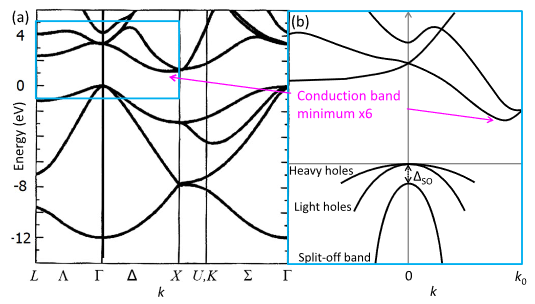
\includegraphics[width=\columnwidth]{bandstructure}
\caption{
bandstructure
}
\label{fig:bandstructure}
\end{figure}
 


\begin{figure}
\centering
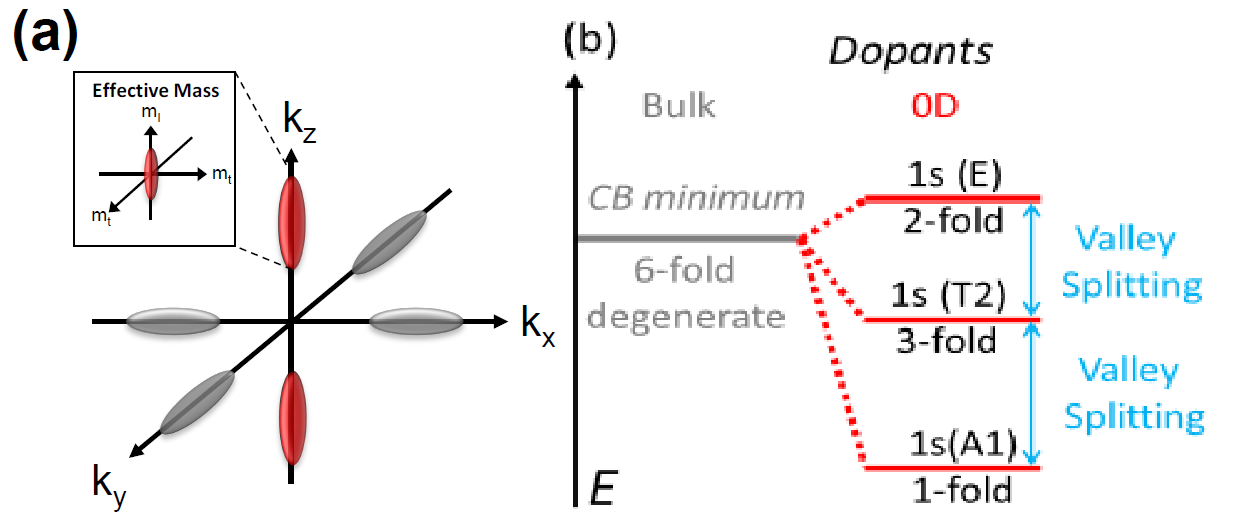
\includegraphics[width=\columnwidth]{SiValleys}
\caption{
Valleys in silicon. (a) Conduction band band minima in bulk silicon, showing six ellipsoids
(valleys) in the Brillouin zone. Inset : The components of the effective masses (for the valley kz ), along three
directions in k-space, highlighting the longitudinal (ml ) and transverse (mt ) masses. (b) The degeneracy
of the 6 valleys broken by confinement, strain and sharp interfaces, highlighting the orbital ground states
separated by valley splitting. 
}
\label{fig:sivalleys}
\end{figure}
 

\subsection{The Phosphorus donor spin qubit} \label{sec:donorqubit}

Spin is an intrinsic quantum mechanical property of elementary particles and atomic nuclei that describes how the particle is deflected when moving in magnetic fields. It gives the particle angular momentum and a small magnetic moment. Spin is quantized, thus can only take discrete values $-s, -s+1, ..., s-1, s$ where $s=\frac{n}{2}$ is the spin quantum number with $n\in \mathds{N}_0$. This makes spin $s=1/2$ ideal for quantum computation, being a natural two level system. 
A particle with spin $1/2$ is the electron. The excess electron of a donor in silicon can be used for this purpose. In this environment the donor atom in the semiconductor can be treated analogous to a hydrogen atom in vacuum with a few modifications \cite{Zwanenburg}.
E.g. due to the broken symmetry the dispersion relation for electrons near the bottom of each valley is anisotropic and is described by two light traverse effective masses (mt = 0.19m0) and a heavy longitudinal effective mass (ml = 0.98m0), where mo is the mass of the free electron \cite{d}. This is illustrated in figure \ref{fig:sivalleys} (a).  


\begin{figure}
\centering
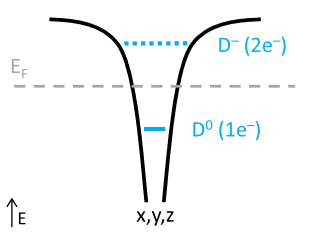
\includegraphics[width=0.5\columnwidth]{confinement}
\caption{
Donor confinement potential. 
}
\label{fig:donorconfinement}
\end{figure}


Phosphorus is a convenient donor for silicon as its nucleus also carries spin $1/2$ which gives us a second qubit "for free". 
The spin states $\pm \frac{1}{2}$ of the electron and the nucleus will be called $\{\ket{\uparrow}$, $\ket{\downarrow}\}$ and $\{\ket{\Uparrow}$, $\ket{\Downarrow}\}$ respectively. Unperturbed these spin states have the same energy - they are degenerate. However, if an external magnetic field $B_0$ is applied they split by the Zeeman energy $E_z=\gamma B_0$, with $\gamma$ being the corresponding gyromagnetic ratio, making them accessible as qubits. The Hamiltonian describing this system is 
\begin{equation}
H_Z=\gamma_e B^z_0 \mb{S}_z-\gamma_N B_0^z \mb{I}_z
\end{equation}
with $B_0^z$ as the component of the magnetic field along the z-axis, $\{\mb{S}_z,\mb{I]}_z\}$ the spin operator in z direction of the electron and nucleus respectively and $\gamma_e=28\,$GHz/T, $\gamma_N=17\,$MHz/T as the respective gyromagnetic ratios.

However, the electron and the nucleus are not separated from each other but interact intrinsic due to the hyperfine interaction $A$. This interaction arises from the wave function overlap of the singlet electron ground state A1 and the nucleus and adds an interaction term $A\mb{S\cdot I}$ to the Hamiltonian

\begin{equation}
H=H_z+H_A=\gamma_e B^z_0 \mb{S}_z-\gamma_N B_0^z \mb{I}_z + A\mb{S\cdot I}
\end{equation}
The excited electron valley states have zero probability at the nucleus and thus do not exhibit hyperfine interaction. 
For the conditions $\gamma_eB_0^z \ll A>\gamma_N B_0^z $ which imply that the detuning between the coupled states $\ket{\uparrow\Downarrow},\ket{\downarrow\Uparrow}$ is much larger than the hyperfine coupling, the electron and nuclear states can be separated and the eigenstates of the Hamiltonian $\ket{\uparrow\Uparrow},\ket{\uparrow\Downarrow},\ket{\downarrow\Uparrow},\ket{\downarrow\Downarrow}$ are the tensor products of the individual spin states $\ket{\uparrow\Uparrow}=\ket{\uparrow}\otimes\ket{\Uparrow}$ etc. 
In figure \ref{fig:energydiagram} the energy levels of the eigenstates are displayed. 

\begin{figure}
d
\end{figure}


\subsection{Electron qubit initialization and measurement}\label{sec:qubit_initMeas}
\footnote{The nuclear qubit can be mapped onto the electron with pulses discussed in the paragraph "Qubit control" and thus relies on the same principles.}
To successfully operate the spin system as qubits, one needs to be able to determine in which spin state it is at any given time. To achieve this, we convert the electron spin signal into a charge signal, known as spin to charge conversion and then electrically read out the charge signal with off the shelve electronics.

To convert from spin to charge the spin states of the electron are tuned with bias voltages such that the Fermi level of a neighbouring reservoir lies in between both states like shown in figure \ref{fig:spintocharge}. In this case $\ket{\uparrow}$ will tunnel into the reservoir and be replenished by $\ket{\downarrow}$ while $\ket{\downarrow}$ will stay at the donor. As this tunnel process is a moving charge, we have now converted the spin signal into a charge signal. 

The key feature to now readout this charge signal is the single electron transistor (SET). This is a nanometric structure which can form an island of hundreds of electrons. The island is capacitively coupled to a top gate and tunnel coupled to source and drain reservoirs as shown in figure \ref{fig:SET}. The energy of this island is 
\begin{align*}
E & =  \frac{Q^2}{2C}\\
& =  \frac{e^2N^2}{2C}\\
& =  E_C N^2
\end{align*}
where Q is the charge of island which consists out of N electrons, C is the total capacitance of the dot and $E_C$ the charging energy. 
To add one electron one needs the energy 
\begin{align*}
\Delta E(N)& =  E(N+1)-E(N)\\
 & =  E_C\left(N+\frac{1}{2}\right)
\end{align*}
also called the electrochemical potential $\mu(N)$. Transport, thus current flow, occurs when the electrochemical potential to add the Nth electron lies between the Fermi levels of the source and drain reservoirs as shown in figure \ref{fig:SET2}. If transport is blocked, the SET is in Coulomb blockade. By varying the top gate voltage oscillations between high and low current occurs when single electrons tunnel, which are called Coulomb oscillations and are shown in figure \ref{fig:coulomboscillations}. Due to the sharp slope of these curves, the sensitivity of the SET current to changes in the electrostatic environment is very high. Thus a change in charge on the donor due to a spin tunnelling event will result in a change in current on the SET. Consequently we can readout the electron qubits  spin state. This is shown in figure \ref{fig:blips}. 

This measurement process can also be used to initialize the qubit into a well known state, a vital feature for qubit operation, as at the end of the process always $\ket{\downarrow}$ is occupying the donor. 

This has been first demonstrated on a single electron spin on a phosphorus donor in 2010 by A. Morello who showed single shot readout.\cite{Morello2010}

\paragraph*{Qubit control} \label{sec:qubit_control}
To control the qubits we use magnetic resonance. As mentioned above, spins have a magnetic momentum and react to external magnetic fields. More precisely they precess around the axis of magnetization with a frequency $f_L$, the so called Larmor frequency. Now we apply a magnetic pulse oscillating with a frequency $f_{ac}$. In the reference frame of this oscillating  field, also known as the rotating frame, the spin appears to precess at a frequency $\Delta f=f_L-f_{ac}$.  If a magnetic drive with the same frequency as the Larmor frequency is applied perpendicular to $B_0^z$, it appears in the rotating frame as a static field of amplitude $B_1$ in the x-y plane. If the spin has been prepared in either $\ket{\uparrow}$ or $\ket{\downarrow}$, the spin will rotate around the axis of $B_1$ with frequency $f_{Rabi}=\gamma B_1$, the Rabi frequency, as these rotations are called Rabi oscillations. This is shown in figure \ref{fig:rabi}. 
When this magnetic resonance technique is applied to the electron, we speak of electron spin resonance (ESR) and when it is applied to the nucleus of nuclear magnetic resonance (NMR).
In figure \ref{fig:leveldiagram} these magnetic transitions and their resonance frequencies are illustrated. 
For the phosphorus donor electron qubit this was first demonstrated in 2012\cite{Pla2012} and for the nuclear qubit in 2013.\ref{Pla2013}

%extend more in preparation for flipflop?


\paragraph*{Qubit decoherence} \label{sec:decoherence}

Quantum decoherence is the loss of quantum information from a system, in our case the qubit, to the environment.
This happens as the qubit is never fully isolated from its environment and interactions lead to the transfer of information from the qubit to the outside. 

There are two main parameters which describe the lifetime of the qubits quantum information. 

Firstly, there is the relaxation time $T_1$ which is the time scale on which the qubit decays from its excited state $\ket{\uparrow}$ to its ground state $\ket{\downarrow}$ due a perturbation orthogonal to the quantization axis, in the case of the donor qubit this means a perturbation of type $\sigma_{x,y}$. This perturbations can e.g. arise due to charge fluctuations and tunnelling effects. More about the specific effect of this process on our qubit, its origins and how to mitigate it will be discussed in chapter \ref{chap:t1}. 

Secondly, there is the randomization of the phase of a quantum superposition on the time scale $T_2$, which is called dephasing. Slow perturbations along the quantization axis $\sigma_z$ cause the Larmor frequency to fluctuate and the state starts precessing in the rotation frame such that we loose track of the phase of the state. 
In ensemble measurements a third time scale is relevant, the dephasing time $T_2^*$, where different parts of the ensemble have different Larmor frequencies due to slow fluctuations. As we are working with single spins, we only encounter time ensemble measurements. In these cases the Larmor frequency varies between each measurement due to slow changes in the environment in between. This dephasing can be suppressed by clever pulsing methods like hahn echo and CPMG \cite{CPMG}. 

Both the electron and the nuclear spin have exceptionally long coherence times when placed in an environment with few surrounding spins, as was first measured by J. Muhonen in 2014 \cite{Muhonen2014}. In combination with the high fidelity control, this makes for an excellent qubit.  

%more reference?

%----------------------------------------------------------------------------------------

\section{Approach to large scale quantum computing} \label{sec:scaleup}

\subsection{Surface Code}

\section{Circuit Quantum Electrodynamics}

\section{Scope of this thesis}



% Chapter Template

\chapter{The flip flop qubit} % Main chapter title

\label{Chapter2} % 

\HRule
\vspace{0.5cm} \hspace{2cm}
\small
\hangindent=4cm
\\
        ``\emph{Scalability is the future}"
\\ \\
\hangindent=4cm
\begin{flushright}
--? \\
\end{flushright}

\vspace{0.5cm}

\noindent \HRule
\clearpage

As discussed in chapter \ref{sec:scaleup}, new ideas for long range, scalable coupling are necessary to advance silicon quantum computing. This chapter presents a new type of qubit that relies on electric dipole interactions and aims to answer this demand. 

\section{A new electrically accessible qubit}

\begin{figure}[h]
	\centering
	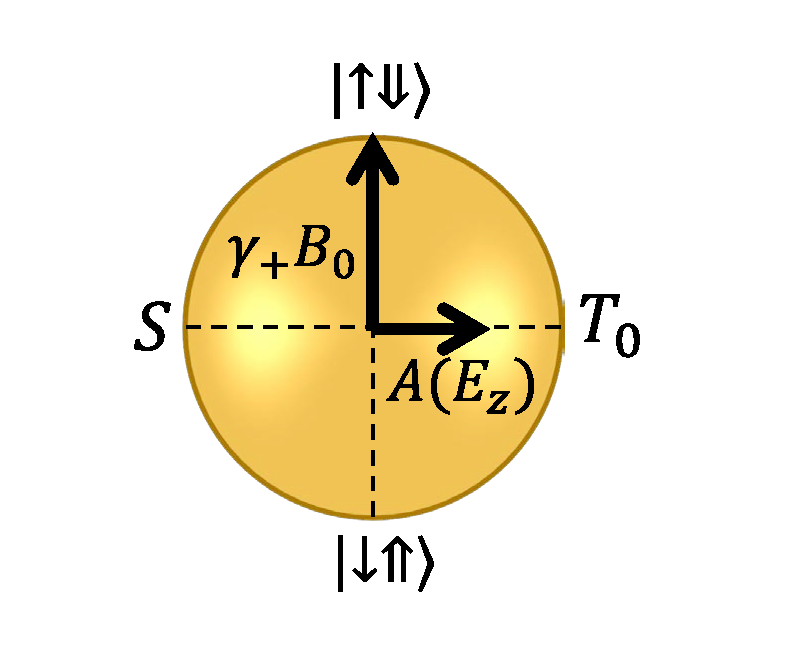
\includegraphics[width=0.5\columnwidth]{polished/ff_blochsphere.pdf}
	\caption[Flip-flop qubit Bloch sphere]{\textbf{Flip-flop qubit Bloch sphere.} Bloch sphere of a flip-flop spin qubit in an external magnetic field $B_0$ coupled to a vertical electric field $E_z$ via the hyperfine interaction $A$. Electron-nuclear singlet and triplet states are denoted by $S=\left(\ket{\downarrow\Uparrow}-\ket{\uparrow\Downarrow}\right)/\sqrt{2}$ and $T_0=\left(\ket{\downarrow\Uparrow}+\ket{\uparrow\Downarrow}\right)/\sqrt{2}$.}
	\label{fig:ff_blochsphere}
\end{figure}

\cite
The new qubit is based on the phosphorus donor qubit as described in section \ref{sec:donorqubit}. However, instead of encoding the quantum information in just the electron or the nuclear spin, we define a new qubit with the anti-aligned spin states $\ket{\downarrow\Uparrow}, \ket{\uparrow\Downarrow}$ as the basis. We call this the flip-flop qubit. This transition is not magnetically accessible as the total z-angular momentum is constant. However, the hyperfine interaction $H=A\bm{S\cdot I}$ is a transverse term for this states with its eigenstates $S=\left(\ket{\downarrow\Uparrow}-\ket{\uparrow\Downarrow}\right)/\sqrt{2}$ and $T=\left(\ket{\downarrow\Uparrow}+\ket{\uparrow\Downarrow}\right)/\sqrt{2}$ (see figure \ref{fig:ff_blochsphere}) and thus can be used to drive the transition. 
The flip-flop qubit energy splitting is 
\begin{equation} \label{eq:e_ff}
\epsilon_{\rm ff}(A)=\sqrt{\left(\gamma_+B_0\right)^2+A^2},
\end{equation}
where $\gamma_+=\gamma_e+\gamma_n$. Is $A$ now modulated at frequency $\epsilon_{ff}$, we are driving the flip-flop transition with electric dipole spin resonance (EDSR). 

The hyperfine interaction strength between the electron and the nucleus depends on the overlap of the electron wave function with the nucleus position $A\sim |\psi(0,0,z_d)|^2$. Hence, by reducing said overlap, the interaction can be decreased. This can be achieved by applying an electric field on top of donor that pulls the electron from the donor to the SiO2 interface, where it behaves like a quantum dot after ionization. The electron charge position is described by the orbital degree of freedom.

\subsection{Manipulating the orbital degree of freedom: the charge qubit} \label{sec:chargequbit}

When the electron is at the donor, the ground orbital wavefunction $\ket{d}$ is a symmetric combination of the 6 valleys $\mathrm{k_{\pm x}}$, $\mathrm{k_{\pm y}} $, $\mathrm{k_{\pm z}} $ (see chapter \ref{sec:silicon}). The next valley-orbit states are $11.7\,$meV higher in energy and thus can be neglected. When the electron is confined at the interface, in a quantum dot like state, in-plane strain splits off the in-plane $k_{\pm x}, k_{\pm y}$ valleys so that the wave function lives in the z valleys $k_{\pm z}$ where the remaining twofold degeneracy is lifted by the electronic z confinement into a lower valley $\ket{i}$ and a higher valley $\ket{v}$. The remainder of the excited donor and dot states are well above the ground states by several meV \cite{Rahman2009, Calderon2009}. Thus, close to the ionization point $E_z^0$, the lowest-energy sates of the system are $\ket{d}, \ket{i}, \ket{v}$ as shown in figure \ref{fig:nemolevels} inset. 
These levels can be computed with atomistic tight binding calculations using the package NEMO-3D \cite{Klimeck2007a, Klimeck2007b} with donor depth $z_d=15.2\,$nm below the Si/SiO2 interface and the donor biased close to ionization. Figure \ref{fig:nemolevels} shows the dependence of the energy levels on the electric field $E_z$ with the dots indicating the tight binding simulations. 

\begin{figure}[h]
	\centering
	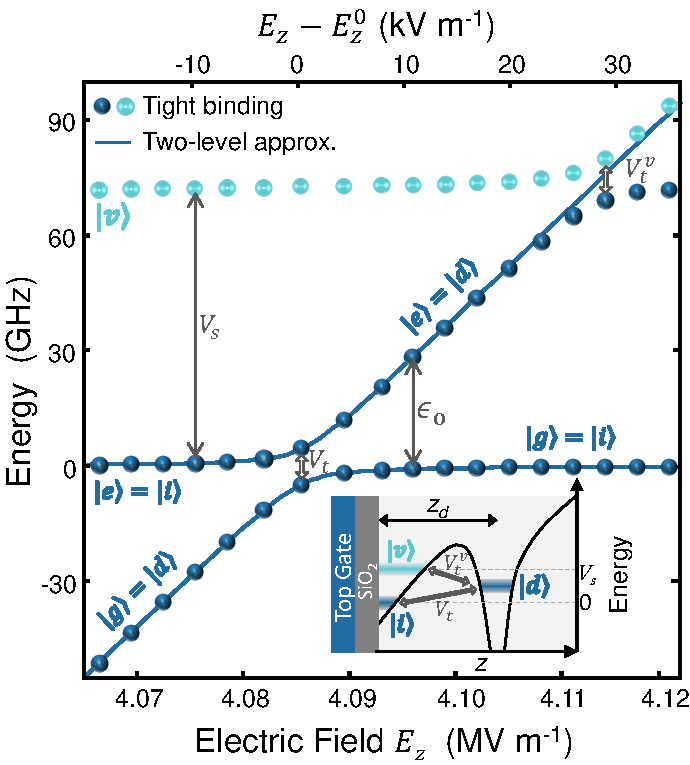
\includegraphics[width=0.7\columnwidth]{Nemolevels}
	\caption[Orbital and valley states]{\textbf{Orbital and valley states.} The lowest orbital energy levels of the donor-interface system, with respect to the lower valley interface state $\lvert i \rangle$ (set as the zero-energy reference). The donor is assumed 15.2 nm below a Si/SiO$_2$ interface. The dots correspond to the energy levels obtained from a full-scale tight-binding calculation with NEMO-3D. Solid lines represent the energy levels obtained from the two level approximation described by Eq. \ref{eq:H_orb}. Inset: Potential profile as a function of depth, illustrating the donor $\lvert d \rangle$, lower $\lvert i \rangle$ and upper $\lvert v \rangle$ valley interface states. The donor ground state is tunnel-coupled to the lower and upper valley interface states by $V_t$ and $V_t^v$  respectively.}
	\label{fig:nemolevels}
\end{figure}

We find that the electron orbital charge qubit degree of freedom can be approximated by a two-level system with ground state $\ket{g}$ and excited state $\ket{e}$ for $E_z<E_z^v\sim 4.11\,$MV/m when the third valley state $\ket{v}$ becomes relevant. 

When $E_z \ll E_z^0$, the charge qubit ground state $\lvert g \rangle $ consists of the electron being  localized at the donor, $\ket{d}$, whereas the first excited state $\lvert e \rangle $ corresponds to the lower valley interface state $\ket{i}$. 
With increasing $E_z$, the two states approach, and anticross at the ionization point $E_z = E_z^0$. For $E_z\gg E_z^0$ $\ket{d}$ is the excited state, until it eventually anticrosses with the upper valley interface state$\ket{v}$ at $E_z^v$. 

We can describe this charge qubit with the Pauli matrices 
\begin{equation}\sigma_x=\begin{pmatrix}0 & 1\\1 &0 \end{pmatrix}, \sigma_y=\begin{pmatrix}0 &-i\\i &0 \end{pmatrix}, \sigma_z=\begin{pmatrix}1 &0\\0 &-1 \end{pmatrix}.
\end{equation} 
Choosing $\ket{d}=\begin{pmatrix}0\\1 \end{pmatrix},\ket{i}=\begin{pmatrix}1\\0\end{pmatrix}$ as the basis states the corresponding Hamiltonian is
\begin{equation} \label{eq:H_orb}
\mathcal{H}_{\rm orb}=\frac{V_t \sigma_x-\left[e(E_z - E_z^0) d/h\right]\sigma_z}{2},
\end{equation}
(solid lines in figure \ref{fig:nemolevels}) with an energy separation between the two levels of 

\begin{equation} \label{eq:e_o}
\epsilon_{\rm o}=\sqrt{\left(V_t\right)^2+\left[e(E_z - E_z^0) d/h\right]^2}.
\end{equation}

where $V_t=9.3\,$GHz is the tunnel coupling between the donor and the interface potential wells (at $z_d=15.2\,$nm), $E_z^0$ is the vertical electric field at the ionization point and $h$ is the Planck constant. The charge qubit transition energy is plotted in figure \ref{fig:chargequbit}.  We find that $d=11\,$nm, which represents the separation between the center-of-mass positions of the donor $\ket{d}$ and interface $\ket{i}$ orbitals, and is expectedly lower than the donor depth $z_d$.

\begin{figure}[h]
	\centering
	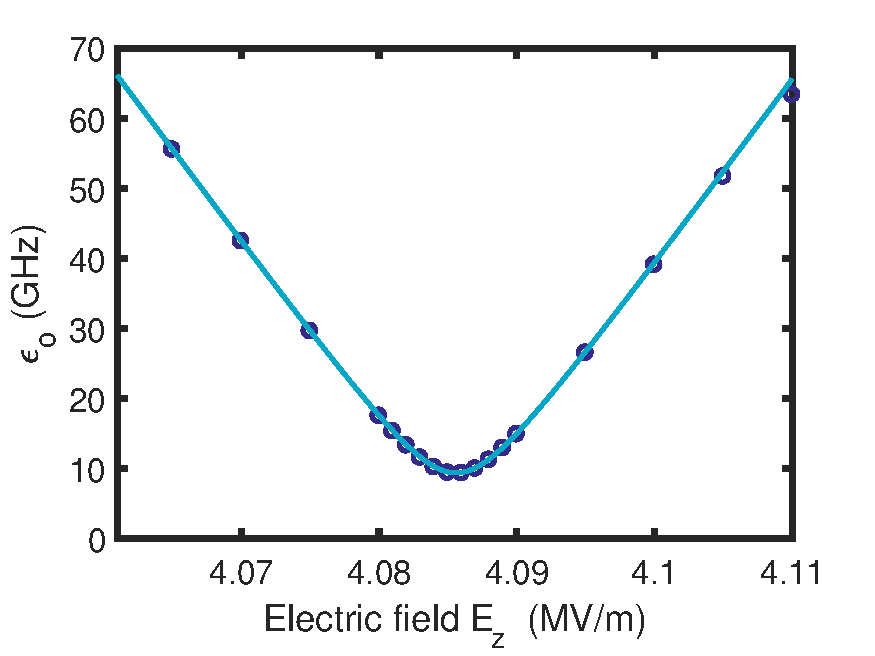
\includegraphics[width=0.8\columnwidth]{polished/chargequbit_dispersion.pdf}
	\caption[Charge qubit dispersion relation]{\textbf{Charge qubit dispersion relation.} Charge qubit dispersion relation $\epsilon_0$ as a function of vertical electric field $E_z$, for $V_t=9.3\,$GHz, $d=11nm$ and $E_z^0=0\,$V. The dots are obtained by NEMO-3D full-scale tight binding simulation while the line corresponds to the two-level approximation, giving eq. \eqref{eq:e_o}.}
	\label{fig:chargequbit}
\end{figure}

At the ionization point $E_z^0$ the basis states of the charge qubit are $\ket{g}=\frac{\ket{i}-\ket{d}}{\sqrt{2}}=\frac{1}{\sqrt{2}}\begin{pmatrix}-1\\1\end{pmatrix}$ and $\ket{e}=\frac{\ket{i}+\ket{d}}{\sqrt{2}}=\frac{1}{\sqrt{2}}\begin{pmatrix}1\\1\end{pmatrix}$ and $\epsilon_0=V_t$. 
If we were to express the charge qubit in this basis, we transform $\sigma_z\leftrightarrow-\sigma_x$ in $H_{orb}$.

More generalized we can express the charge qubit eigenstates as
\begin{eqnarray}\label{eq:chargestates_e}
\ket{e}&=&\alpha_1 \ket{i}+\beta_1\ket{d}=\begin{pmatrix}\alpha_1\\ \beta_1\end{pmatrix}\\
\label{eq:chargestates_g}
\ket{g}&=&\alpha_2 \ket{i}+\beta_2 \ket{d} =\begin{pmatrix}\alpha_2\\ \beta_2\end{pmatrix}
\end{eqnarray} with $\alpha_{1,2},\beta_{1,2}$ depending on $V_t$ and $E_z$. 


\subsection{Modulating the hyperfine interaction} \label{sec:hyperfine_modulation}
 

\begin{figure}[h]
	\centering
	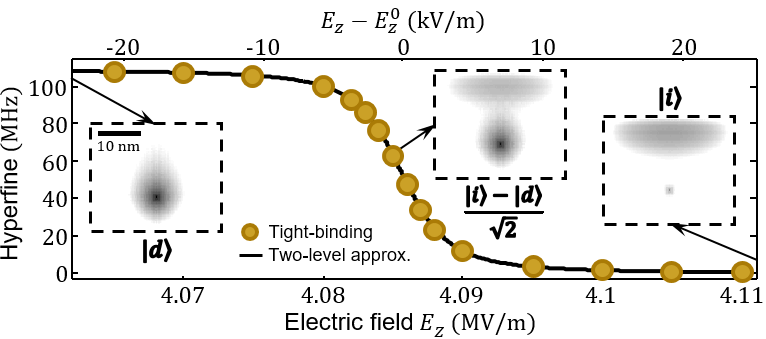
\includegraphics[width=0.9\columnwidth]{hfchange.png}
	\caption[Hyperfine interaction change with electric field]{\textbf{Hyperfine interaction change with electric field} Atomistic tight-binding simulations \cite{Klimeck2007a,Klimeck2007b} (dots) of the electron-nucleus hyperfine interaction, for a $z_d=15.2$~nm deep donor, as a function of vertical electric field. The solid line is a fit using the simplified two-level Hamiltonian $\mathcal{H}_{\rm orb}+\mathcal{H}_A^{\rm orb}$, which yields $V_t=9.3$~GHz (see \ref{fig:nemolevels}). The insets show the electron ground-state wavefunction $\ket{g}$ for three different vertical electric fields.}
	\label{fig:hfchange}
\end{figure}

As the hyperfine coupling the electron and nucleus experience depends on the wave function overlap between electron and nucleus, it depends on the state of the charge qubit. Is the charge qubit in the donor state $\ket{d}$, the hyperfine interaction is full strength $A$ while it is $0$ if the charge qubit is in the interface state $\ket{i}$. Thus we can describe the orbital dependent hyperfine Hamiltonian as 

\begin{equation} \label{eq:H_A}
\mathcal{H}_{A}^{\rm orb}=A\left(\frac{1 - \sigma_z}{2}\right){\bf S\cdot I}
\end{equation}

Figure \ref{fig:hfchange} shows the hyperfine strength with applied electric field. The dots present the tight-binding simulations with NEMO-3D\cite{Klimeck2007a,Klimeck2007b}. The line is derived from the Hamiltonian by calculating the ground state eigenvector $\ket{g}$ and measuring its expectation value 

\begin{equation}\label{eq:AE}
A(E_{dc})=\langle g|A\left(\frac{1 - \sigma_z}{2}\right)|g\rangle=A|\beta_2|^2.
\end{equation}
We find that both methods agree well which confirms our two-level approximation. The insets show the wavefunction at different electric fields. 

To determine the coupling between the charge qubit and the spin states $\ket{\downarrow\Uparrow}, \ket{\uparrow\Downarrow}$ we calculate the matrix transition element 
\begin{equation}\label{eq:g_so}
g_{so}=\langle g\uparrow\Downarrow|H_{A}^{orb}\ket{e\downarrow\Uparrow}=\frac{A}{4}\langle g|\sigma_z\ket{e} =\frac{A}{2}\left(\alpha_1\alpha_2^\dagger-\beta_1\beta_2^\dagger\right)
\end{equation}
At the ionization point $\langle g|\sigma_z\ket{e}=1$ and the coupling is the strongest, allowing for fast driving. To calculate $\langle g|\sigma_z\ket{e}$ outside the ionization point we need to determine $\alpha,\beta$ from equations \eqref{eq:chargestates_e}, \eqref{eq:chargestates_g} by calculating the eigenvectors $\ket{g},\ket{e}$. 

We generalize the problem to 

\begin{equation}
H=\begin{pmatrix}
-A & B\\
B & A
\end{pmatrix}
\end{equation}
where $A=e\frac{\left(E_z-E_z^0\right)d}{2h}$ and $B=\frac{V_t}{2}$.

The eigenvectors are calculated by

\begin{equation}
\begin{pmatrix}
-A-\lambda_{1,2} & B\\
B & A-\lambda_{1,2}
\end{pmatrix} \cdot 
\begin{pmatrix}
\alpha_{1,2} \\ \beta_{1,2}
\end{pmatrix} =
\begin{pmatrix}
0 \\ 0
\end{pmatrix}
\end{equation}

which gives the equations 
\begin{eqnarray}
\left(-A-\lambda_{1,2}\right)\alpha_{1,2}+B\beta_{1,2}=0 \label{eq:eigen1}\\
\alpha_{1,2}A+\left(A-\lambda_{1,2}\right)\beta_{1,2}=0. \label{eq:eigen2}
\end{eqnarray}
Furthermore, we have the normalization condition
\begin{equation}\label{eq:norm}
\beta_{1,2}=\sqrt{1-\alpha_{1,2}^2}.
\end{equation}
We insert equation \eqref{eq:norm} into \eqref{eq:eigen1}, \eqref{eq:eigen2} and get
\begin{eqnarray}
\alpha_{1,2}=\frac{1}{\sqrt{1+\frac{\left(A+\lambda_{1,2}\right)^2}{B^2}}}\\
\beta_{1,2}=\sqrt{1-\frac{1}{1+\frac{\left(A+\lambda_{1,2}\right)^2}{B^2}}}.
\end{eqnarray}

With 
\begin{equation}
\lambda_{1,2}=\pm\sqrt{A^2+B^2}
\end{equation}
follows

\begin{equation}
\label{eq:ab}
\begin{aligned}
\alpha_{1}=\frac{1}{\sqrt{\Phi^2+1}}=\beta_2\equiv\beta\\
\beta_{1}=\frac{\Phi}{\sqrt{1+\Phi^2}}\equiv\alpha\\
\alpha_{2}=\frac{1}{\sqrt{1+\Theta^2}}=-\beta_1=-\alpha\\
\beta_{2}=\frac{\Theta}{\sqrt{1+\Theta^2}}=\beta
\end{aligned}
\end{equation}

where 
\begin{equation}
\label{eq:abcont}
\begin{aligned}
\Phi=\frac{A+\sqrt{A^2+B^2}}{B}\\
\Theta=\frac{A-\sqrt{A^2+B^2}}{B}.
\end{aligned}
\end{equation}


This gives us the hybridized states 
\begin{equation}
\label{eq:hybridstates}
\begin{aligned}
\ket{e}&=&\beta \ket{i}+\alpha\ket{d}\\
\ket{g}&=&-\alpha \ket{i}+\beta \ket{d}.
\end{aligned}
\end{equation}



Now we can calculate $A(E_{dc})$ with equation \eqref{eq:AE} to
\begin{equation}
A(E_{dc})=A\left(\frac{\Theta}{\sqrt{1+\Theta^2}}\right)^2=\frac{A}{2}\left(1-\frac{e\left(E_z-E_z^0\right)d/h}{\epsilon_0}\right).
\end{equation}

and the coupling rate \eqref{eq:g_so} to
\begin{equation}
g_{so}=\frac{A}{4}\frac{V_t}{\epsilon_0}.
\end{equation}

Here we have assumed that the hyperfine coupling between electron spin and $^{31}$P nucleus is purely isotropic \cite{Feher1959}, i.e. dominated by the Fermi contact hyperfine term. This assumption may no longer exactly hold when the donor electron wave function is distorted from its spherical symmetry in the presence of the strong vertical electric field, whereby a small dipolar component can be created (a related case, where the electron is shared between two proximal P donors, has been recently studied \cite{Hile2018}). However, it is known that the Fermi contact component of the hyperfine coupling for donors in silicon is always the dominant term, even for $^{29}$Si nuclei which are placed off-center with respect to the symmetry point of the wavefunction \cite{Ivey1975}. Therefore, we expect the isotropic approximation to capture the main physics of the problem.


\subsection{The flip-flop qubit} \label{sec:flipflop}

As we apply an external magnetic field $B_0$ to our system, we need to account for the Zeeman energy of both the electron and the nuclear spin. This energy depends on the gyromagnetic ratio. However, the electron gyromagnetic ratio $\gamma_e$ changes when the electron is confined at the Si/SiO2 interface, up to $0.7\%$ from the donor-bound electron \cite{Rahman2009}. We include this in the Zeeman Hamiltonian

\begin{equation} \label{eq:H_Zeeman_orb}
\mathcal{H}_{B_0}^{\rm orb}=\gamma_e B_0\left[1+\left(\frac{1+\sigma_z}{2}\right)\Delta_\gamma\right]S_z - \gamma_n B_0 I_z.
\end{equation}

Thus to describe the full physics of the flip-flop qubit we get

\begin{equation} \label{eq:H_ff_ge}
\mathcal{H}_{\rm ff} = \mathcal{H}_{B_0}^{\rm orb} +\mathcal{H}_{A}^{\rm orb} + \mathcal{H}_{\rm orb}.
\end{equation}

This system is composed of the three degrees of freedom, orbital, electron spin and nuclear spin which gives us a eight-dimensional Hamiltonian of
\begin{equation}
\mathcal{H}_{\rm{ff}}=\mathcal{H}_{\rm{orb}}\otimes \mathcal{H}_{\rm{e}}\otimes \mathcal{H}_{\rm{n}}
\end{equation}
with the unperturbed energy eigenstates $\{\ket{g}, \ket{e}\} \otimes \{\ket{\Uparrow}, \ket{\Downarrow}\} \otimes  \{\ket{\uparrow}, \ket{\downarrow}\}$ with the spin states pointing along the external magnetic field. 
As long as the Zeeman energy exceeds the hyperfine modulation characterized by $A/4$, the latter is a perturbation only and the energy eigenstates of $\mathcal{H}_{\rm{ff}}$ remain the approximate products of the eigenstates. 

\begin{figure}[h]
	\centering
	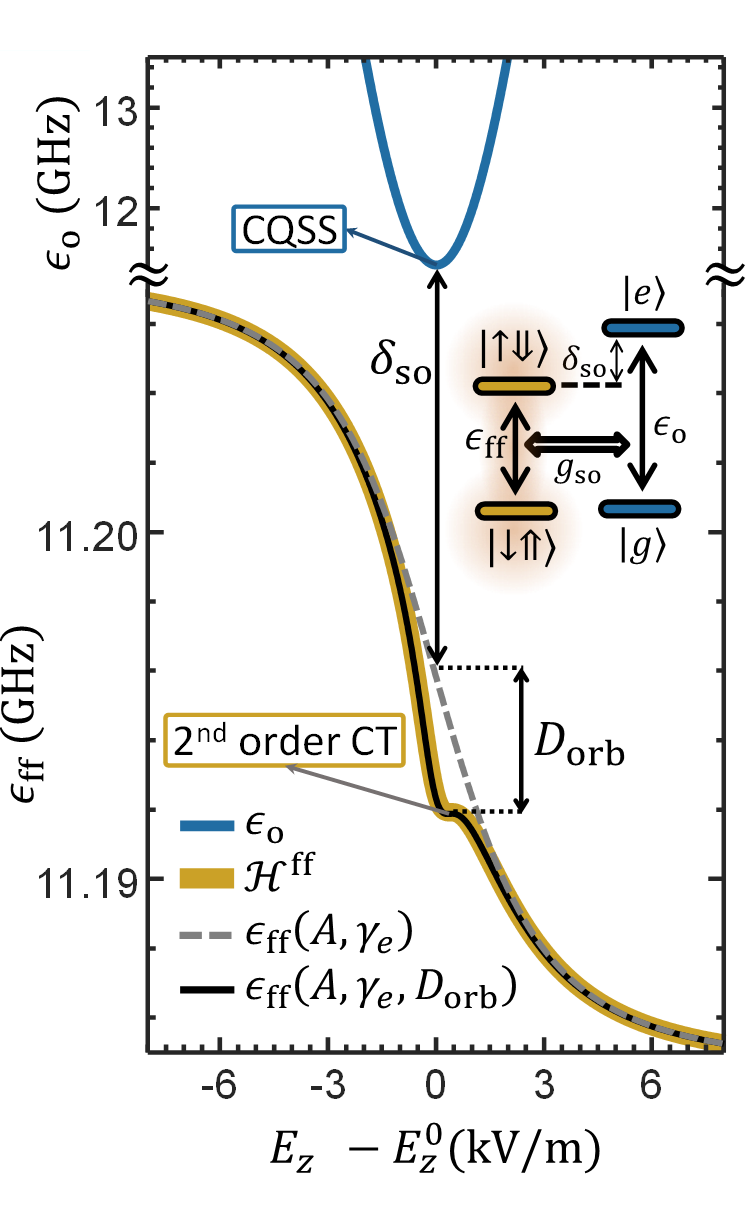
\includegraphics[width=0.6\columnwidth]{polished/ff_energy.png}
	\caption[Flip-flop qubit dispersion relation]{\textbf{Flip-flop qubit dispersion relation} Charge, $\epsilon_{\rm o}$, and flip-flop, $\epsilon_{\rm ff}$, qubits transition frequencies as a function of vertical electric field $E_z$, for $B_0=0.4$~T, $A=117$~MHz, $d=15$~nm, $\Delta_\gamma=-0.2\%$ and $V_t=11.44$~GHz. The inset shows the level diagram of flip-flop states coupled to charge states. CT stands for 'clock transition' and CQSS for 'charge qubit sweet spot'.}
	\label{fig:ff_energy}
\end{figure}

To calculate the flip-flop qubit transition energy we numerically determine the eigenvectors of $\mathcal{H}_{\rm{ff}}$ and find the ones with the largest overlap to the flip-flop states $\ket{g \Downarrow \uparrow}, \ket{g\Uparrow\downarrow}$ with the orbital state remaining unexcited. We then  compute the flip-flop qubit transition energy by calculating the difference of the corresponding eigenvalues. Thus we arrive at the curve plotted in yellow in figure \ref{fig:ff_energy}.

When we compare these results to the bare flip-flop energy $\epsilon_{\rm{ff}}(A,\gamma_e)$ \eqref{eq:e_ff} (plotted in dotted grey in figure \ref{fig:ff_energy}) we find a large deviation around the ionization point. $\epsilon_{\rm{ff}}(A,\gamma_e)$ shows a steep slope, mostly caused by the $E_z$-dependence of $\gamma_e$ as $\gamma_+B_0\gg A$ while $\mathcal{H}_{\rm{ff}}$ sees a dip. This dip is a result of the transverse coupling between the charge and spin states created by the hyperfine coupling in $H_{\rm{orb}}^A$. 

The insert in figure \ref{fig:ff_energy} shows the energy levels for our qubit system. On the one hand, we have the charge qubit states $\ket{g}$ and $\ket{e}$ and on the other the spin flip-flop states $\ket{\downarrow\Uparrow}$ and $\ket{\uparrow\Downarrow}$ which are separated by $\epsilon_0$ and $\epsilon_{\rm{ff}}$ respectively. Thus the charge and flip-flop qubit are detuned by $\delta_{\rm so}=\epsilon_{\rm o} - \epsilon_{\rm ff}$ but coupled with strength $g_{so}$. 

\begin{figure}[h]
	\centering
	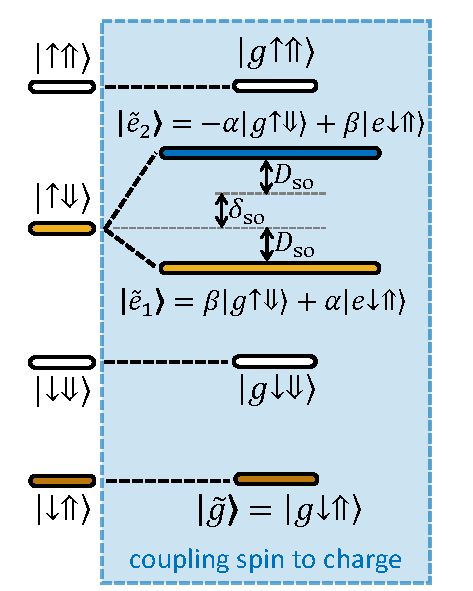
\includegraphics[width=0.5\columnwidth]{polished/hybridlevels.pdf}
	\caption[Hybridized charge-flip-flop states]{\textbf{Hybridized charge-flip-flop states} Level diagram showing the hybridization of the charge and flip-flop states due to the coupling $g_{so}$ when the detuning $\delta_{so}$ is small.}
	\label{fig:hybridlevels}
\end{figure}

For small detunings the coupling leads to a hybridization of the charge and spin states as shown in figure \ref{fig:hybridlevels} with the ground state $\ket{\tilde{g}}$ and two hybridized charge-spin excited states

\begin{equation}
\label{eq:ff_hybrid}
\begin{aligned}
\ket{\tilde{g}}=\ket{g\downarrow\Uparrow}\\
\ket{\tilde{e}_1}=\beta\ket{g\uparrow\Downarrow}+\alpha\ket{e\downarrow\Uparrow}\\
\ket{\tilde{e}_2}=-\alpha\ket{g\uparrow\Downarrow}+\beta\ket{e\downarrow\Uparrow}.
\end{aligned}
\end{equation}
We can determine these eigenvectors analytically by using eq. \eqref{eq:ab} and \eqref{eq:abcont} with $A=\delta_{so}$ and $B=2g_{so}$.  Here A describes the energy scale ($\sigma_z$) and B drives the transitions ($\sigma_x$). 

Due to the detuning the flip-flop transition is a second-order process. Furthermore, as $g_{\rm so}\ll \delta_{\rm so}$, the system is in the dispersive regime. This means that the flip-flop transition experiences an AC Stark shift which can be calculated with second order perturbation theory to

\begin{equation}
\label{eq:Dorb}
\begin{aligned} 
D_{\rm orb}(E_z)&=\frac{\left| \langle \uparrow\Downarrow g|H_{orb}^A\ket{e\downarrow\Uparrow}\langle e\downarrow\Uparrow|H_{orb}^A\ket{g\uparrow\Downarrow}\right|}{E_{e\downarrow\Uparrow}-E_{g\uparrow\Downarrow}}\\
&=\frac{[g_{\rm so}(E_z)]^2}{\delta_{\rm so}(E_z)},
\end{aligned}
\end{equation}

\cite{Blais2004}, reducing the flip-flop qubit frequency to:

\begin{equation} \label{eq:e_ff_ge_Dorb}
\epsilon_{\rm ff}(A,\gamma_e,D_{\rm orb})=\epsilon_{\rm ff}(A,\gamma_e)-D_{\rm orb}(E_z).
\end{equation}

Around $E_z\approx E_z^0$ the charge qubit comes closet to the flip-flop qubit (see Fig. \ref{fig:ff_energy} while the coupling $g_{\rm so}$ is highest. Consequently $D_{\rm orb}(E_z)$ is largest. Plotting Eq.~\eqref{eq:e_ff_ge_Dorb} (thin black line in Fig. \ref{fig:ff_energy}a) agrees with the full numerical simulations of the Hamiltonian in Eq. \eqref{eq:H_ff_ge}. 


\section{Electrical noise and relaxation} \label{sec:noise}

\subsection{Dephasing due to electrical noise} \label{sec:ff_dephasing}

Since our qubit is based on the use of electric fields, the presence of electric noise is a concern for the longevity of our qubit states. Generally, to achieve a high qubit performance one needs a high ratio of qubit coherence time to qubit gate operation time. 

For the charge qubit we find that at the ionization point, the transition frequency exhibits a local minima equal to $V_t$ and is thus first order insensitive to electrical noise $\partial\epsilon_{\rm o}/\partial E_z=0$ (see figure \ref{fig:chargequbit}), called a clock transition. However, we do not intent to operate the charge qubit as its dephasing rate still exceeds $10^6\,$Hz. 

\begin{figure}[h]
	\centering
	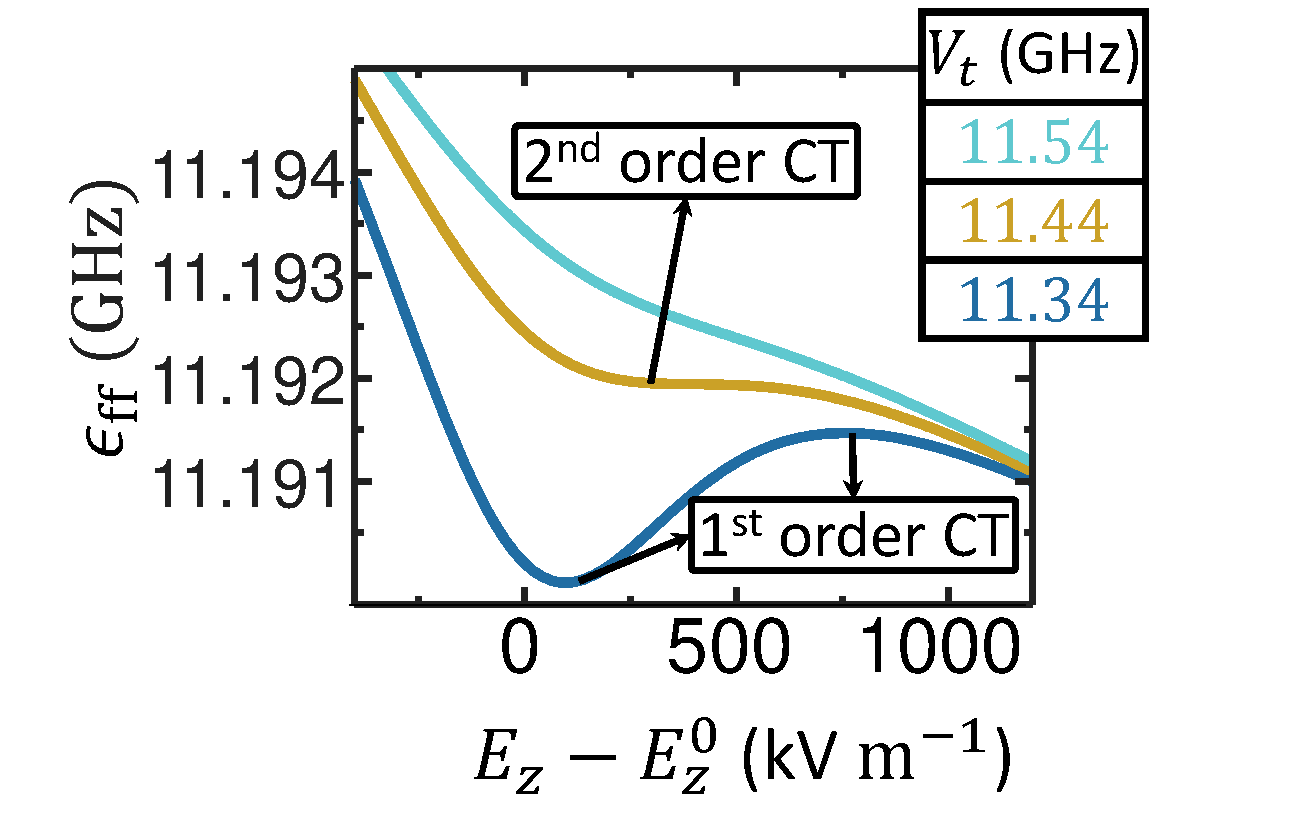
\includegraphics[width=0.75\columnwidth]{polished/ff_Vt.pdf}
	\caption[Flip-flop dispersion for different tunnel couplings]{\textbf{Flip-flop dispersion for different tunnel couplings} $E_z$-dependence of flip-flop precession frequency for the three indicated tunnel coupling values.}
	\label{fig:ff_Vt}
\end{figure}


Conveniently, the flip-flop qubit also exhibits a noise insensitive region close to the ionization point. The properties of this region depend on $V_t$. Figure \ref{fig:ff_Vt} shows 3 different values of $V_t$. For low $V_t$ the dispersive shift is strong due to the closeness of the charge qubit and thus creates two first order clock transitions. These merge into one for $V_t=11.44\,$GHz. This creates a second-order clock transition and strongly reduces dephasing. Finally, for high $V_t$ the dispersive shift is not strong enough and does not yield a minimum. 

We estimate the dephasing from quasi-static $E_z$ noise. This is noise with a spectral weight centred at frequencies smaller than the qubit resonance and Rabi frequency, aligned with the donor-dot direction. We assume $E_{z, rms}^{\rm noise}=100\,$V/m  which corresponds to $1.5\,\mu$eV charge detuning noise for $d=15\,$nm. This is based on the following assumptions. 

\paragraph{Si/SiO2 noise characteristics} 

The Si/SiO$_2$ interface is known to contain a number of defects and electron traps, which can generate charge noise and therefore degrade the operation of qubits sensitive to electric fields. Some experimental studies have extracted the trap density, in the middle of the silicon band gap, for the MOS devices we consider here \cite{Johnson2010}. It is known, experimentally and theoretically, that these charge fluctuators yield a $1/\nu$ frequency dependence of the noise spectral density \cite{Paladino2014}. These models capture the averaged collective effect of many charge fluctuators on the qubit operation. In specific cases, one can occasionally encounter individual charge traps or fluctuators whose effect is more drastic than that of an overall $1/\nu$ noise. However, it is usually possible experimentally to tune the electrostatic landscape of a nanoscale device in such a way that the individual trap is frozen, \textit{i.e.} does not change its charge state while the qubit is operated. This results in a static shift in the local electric field that can be compensated with other gate voltages. In very rare occasions, a charge trap cannot be frozen while placing the qubit at its optimal operation point. In that case, the qubit will have to be considered faulty, and excluded from participating in the operations of the quantum processor.

In the general case where charge noise can be considered an average collective effect, it can be thought of as a quasi-static drift of the qubit electrostatic environment. Indeed, since individual gates take less than a microsecond, the qubit environment is usually static within a single gate, but fluctuates in between gates. The dephasing time $T_2^*$ characterises the influences of these fluctuations on the qubit (see chapter \ref{sec:decoherence}). Experimentally, average quasi-static charge detuning noises around 1-9~$\mu$eV are typically found in a range of semiconductor nanodevices, including SiGe \cite{Kim2015,Thorgrimsson2017,Freeman2017}, AlGaAs \cite{Dial2013} and Si/SiO$_2$ \cite{Harvey-Collard2017,Freeman2017}. In particular, MOS structures were found recently \cite{Freeman2017} to have a charge noise spectrum similar to SiGe devices, around $(0.5~{\mu \rm eV})^2/\nu$. Integrating over a quasi-static bandwidth relevant to experimental time-scales, say between 1 Hz  and 1 MHz, yields 1.7~${\mu \rm eV}$ noise. In our simulations, given that the distance between the donor and interface sites is $\sim10$-30~nm, a noise field of 100~V~m$^{-1}$ would correspond to 1-3~$\mu$eV charge detuning noise. 

\paragraph{Dephasing}

\begin{figure}[h]
	\centering
	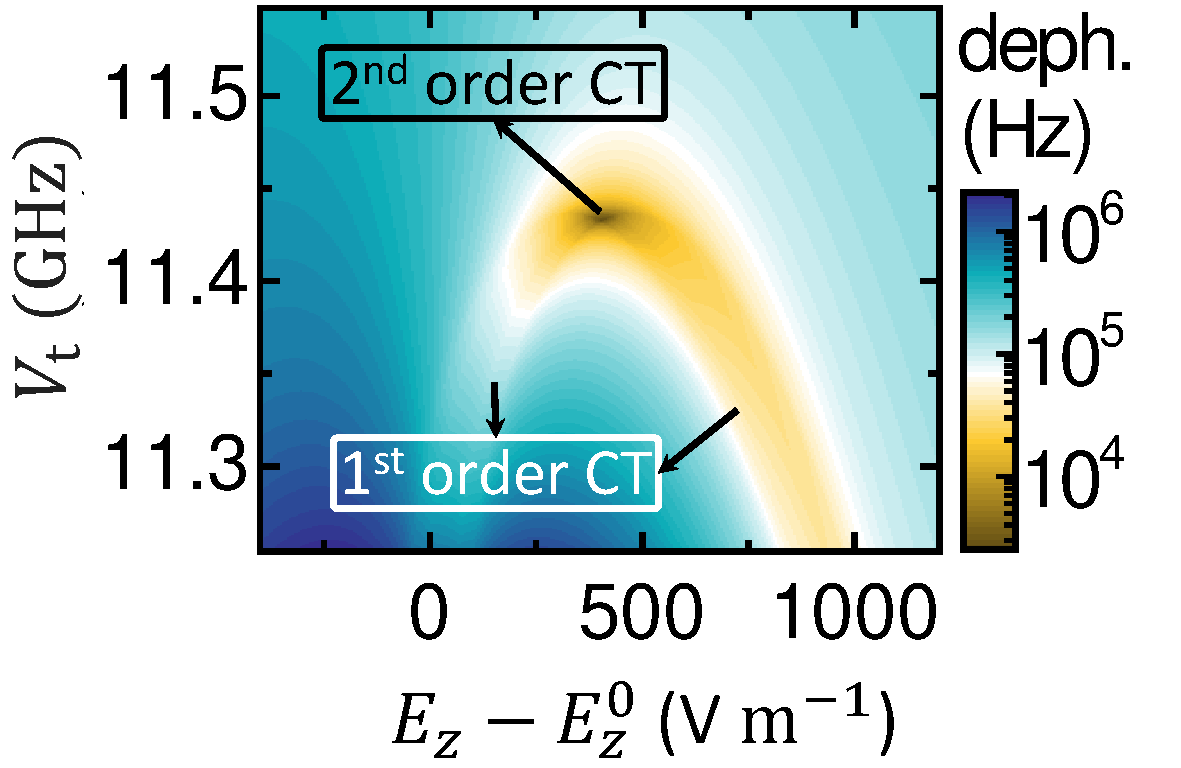
\includegraphics[width=0.65\columnwidth]{polished/ff_dephasing.pdf}
	\caption[Flip-flop dephasing]{\textbf{Flip-flop dephasing} Estimated flip-flop qubit dephasing rate, assuming electric field noise $E_{z, \rm rms}^{\rm noise}=100$~V~m$^{-1}$.}
	\label{fig:ff_dephasing}
\end{figure}

To estimate the dephasing resulting from this charge noise, we calculate the difference between the flip-flop transition frequency $\epsilon_{\rm ff}$ (transition between eigenstates closest to $\ket{g\downarrow\Uparrow}$ and $\ket{g\uparrow\Downarrow}$) and the transition frequencies $\epsilon_{\rm ff}^n$ that result when applying a uniformly distributed noise in the range $E_z^n=\sqrt{3}[-E_{z,\rm rms}^{\rm noise},E_{z,\rm rms}^{\rm noise}]$. This gives 

\begin{equation} \label{eq:dephasing_rate}
{\rm Dephasing~rate}=\sum\limits_{n}{\left|\epsilon_{\rm ff}-\epsilon_{\rm ff}^n\right|/N_n},
\end{equation}

where $N_n$ is the number of sampled $E_z^n$ and $\epsilon_{\rm ff}^n$ is calculated for each value of $E_z^n$. The resulting dephasing rates are shown in figure \ref{fig:ff_dephasing}. 

The rates can be as low as $1/T_2^{\ast} \approx 3$~kHz when at the second order clock transition. This is comparable to the dephasing of $1/T_2^{\ast} \approx 1$~kHz due to magnetic noise in our qubits \cite{Muhonen2014}. 

\subsection{Relaxation}

Relaxation can also inhibit qubit performance (see chapter \ref{sec:decoherence}). In silicon bulk donors the electron spin lattice relaxation time is $T_1\gg 1\,$s due to very weak coupling between the phonons and the spins. However, according to Ref. \cite{Boross2016},  for the charge and the flip-flop qubit the difference in valley population between the interface and donor state causes a potential energy difference that leads to an effective electron-phonon coupling and to relaxation, even for a uniform phonon-induced relaxation. Basically, the relaxation is "valley-enhanced" due to the non-trivial valley structure of the electron-phonon interaction. The charge qubit relaxation rate is $1/T_{1,c}\approx 0.49\,$MHz at the ionization point and increases with higher $\epsilon_0$. 
In the dispersive regime $\delta_{\rm so}\gg g_{\rm so}$ the flip-flop relaxation directly relates to the charge qubit relaxation. It is equal to the amount of charge excited state in the flip-flop eigenstates times the charge qubit relaxation rate which gives

\begin{equation}\label{eq:T1ff}
{1}/{T_{1,\rm ff}}=\left({g_{\rm so}}/{\delta_{\rm so}}\right)^2/{T_{1,\rm o}},
\end{equation}
with 
\begin{equation}\label{eq:T1o}
{1}/{T_{1,\rm c}}=\Theta\epsilon_{\rm o}{V_t}^2,
\end{equation}
where $T_{1,\rm c}$ is the charge qubit lifetime and $\Theta\approx2.37\times10^{-24}~{\rm s}^2$ is determined by the silicon crystal properties \cite{Boross2016}.

\begin{figure}[h]
	\centering
	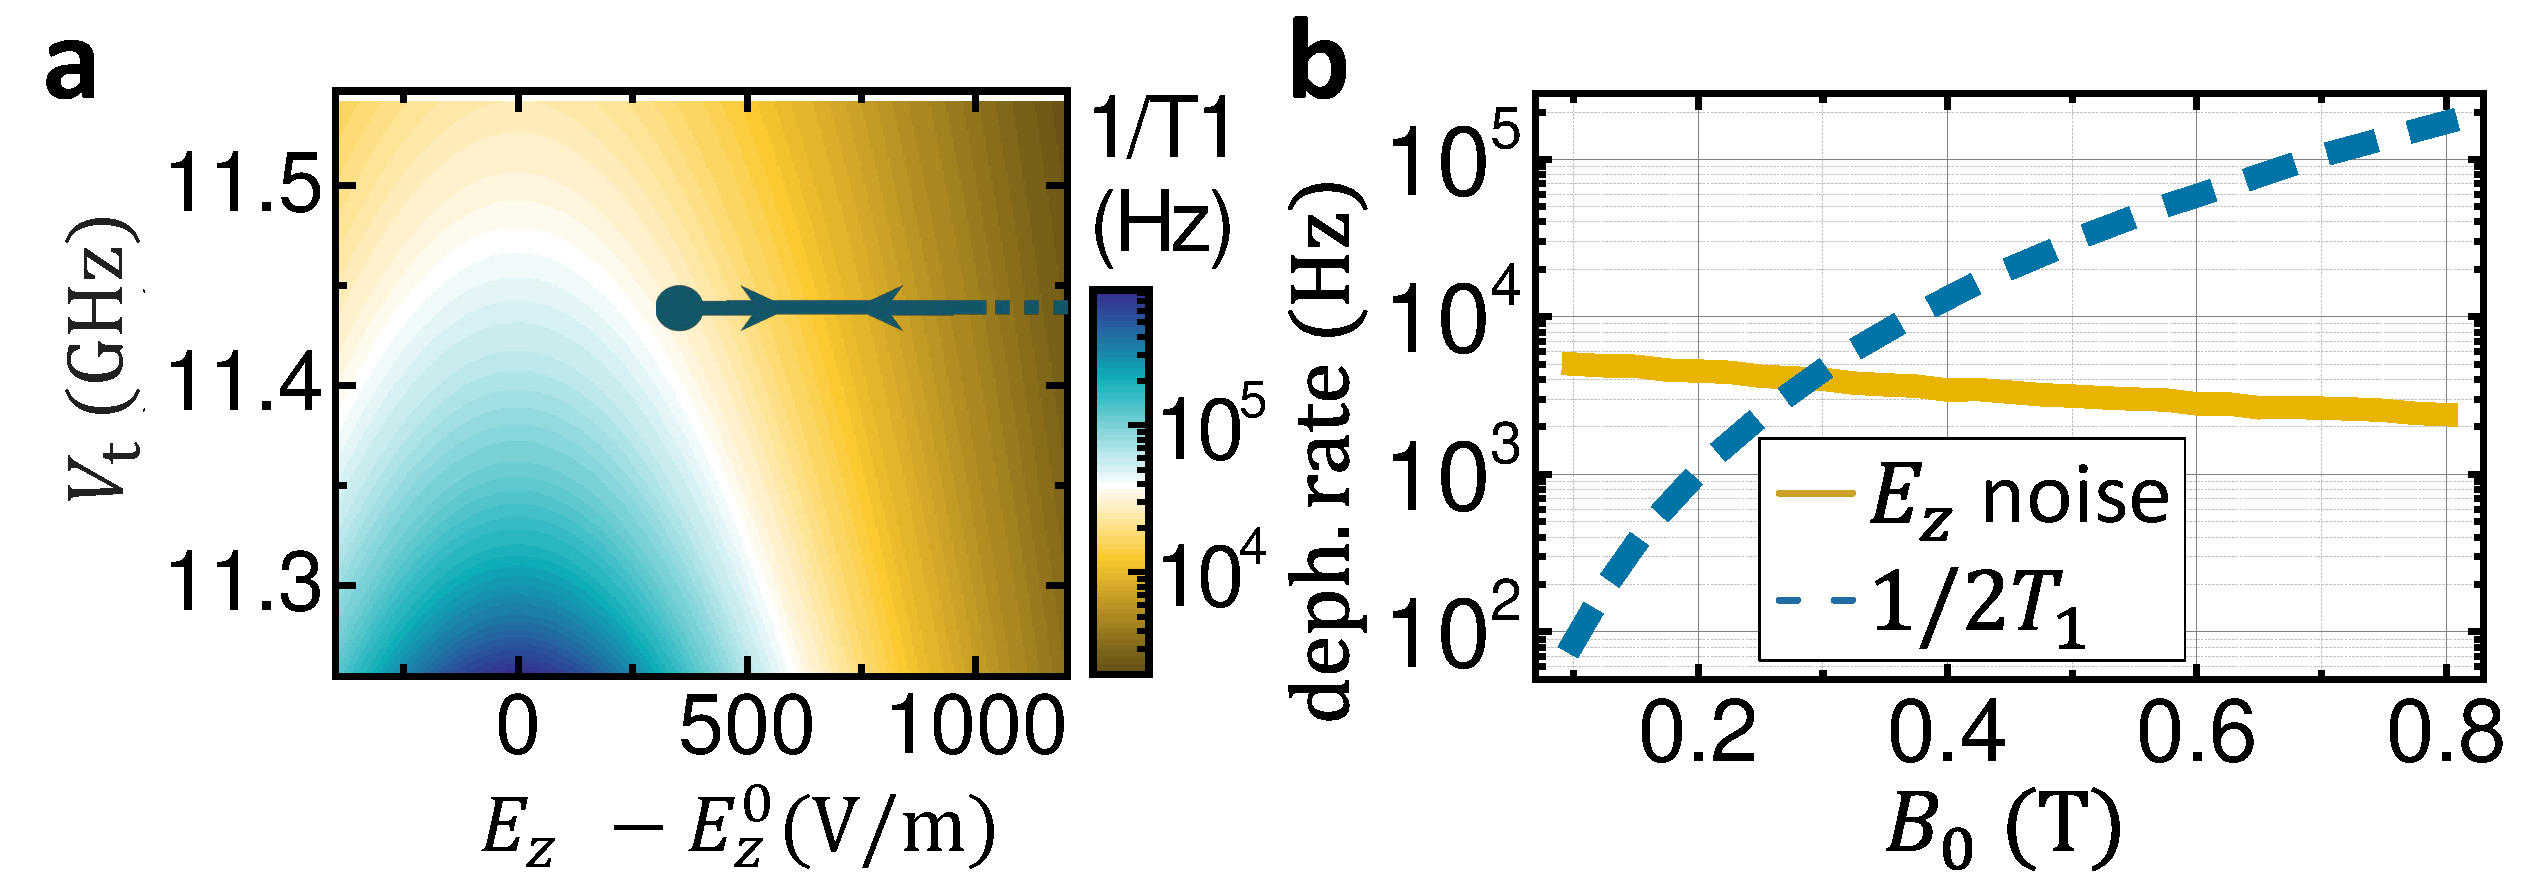
\includegraphics[width=1\columnwidth]{polished/ff_T1.pdf}
	\caption[Flip-flop relaxation rate]{\textbf{Flip-flop relaxation rate. a }Flip-flop qubit relaxation rate, with arrows indicating the adiabatic path used for $z$-gates. \textbf{b} Flip-flop qubit dephasing rate due to $E_z$ noise and relaxation, at $2^{\rm nd}$-order CTs for each $B_0$.}
	\label{fig:T1}
\end{figure}

Figure \ref{fig:T1}a shows the flip-flop relaxation rate depending on the tunnel coupling and the applied electric field. The larger the detuning, the smaller is the component of admixed excited eigenstate $\ket{e\downarrow\Uparrow}$ and consequently the relaxation. At our proposed operating point at the second order clock transition, the relaxation rate is ${1}/{T_{1,\rm ff}}\sim 10\, $kHz. This indicated that the qubit dephasing will be relaxation limited $1/T_2^*=1/2T_1$. However, the relaxation rate depends on the external magnetic field with the power-law relation $1/T_{1,\rm{ff}}\sim B^3$\cite{Boross2016}. Thus reducing the magnetic field, suppresses the relaxation strongly. Figure \ref{fig:T1}b shows the dephasing due to electric noise and relaxation. We find that for $B_0<0.3\,$T, the dephasing is no longer $T_1$ dominated. 


\subsection{Tunnel coupling tuning}

Tuning the flip-flop qubit, e.g. into a clock transition, requires the ability to tune the tunnel coupling $V_t$. $V_t$ is difficult to control at the fabrication stage, given its exponential dependence on donor depth, together with oscillations at the atomic scale \cite{Calderon2009} arising from a similar valley interference effect as the one afflicting the exchange interaction \cite{Koiller2002}. 

Ion-implanting a donor at $z_d \approx 15$~nm below the interface happens with a vertical uncertainty of order $\pm 10$~nm (ref.~\cite{VanDonkelaar2015}), resulting in more than 2 orders of magnitude uncertainty in $V_t$ (ref.~\cite{Calderon2009}). Therefore, it is crucial to implement a method to tune $V_t$ \emph{in situ}. A possible solution is to displace the location of the interface wavefunction laterally, which in turn modifies the overlap between the donor and interface wavefunctions and therefore reduces $V_t$. This can be done by adding two gates on either side of the top gate which pulls the donor electron to the interface (Fig.~\ref{fig:Vt_tuning}a), in such a way that a relative voltage between the gates can modify the interface lateral potential landscape. 

\begin{figure}[h]
	\centering
	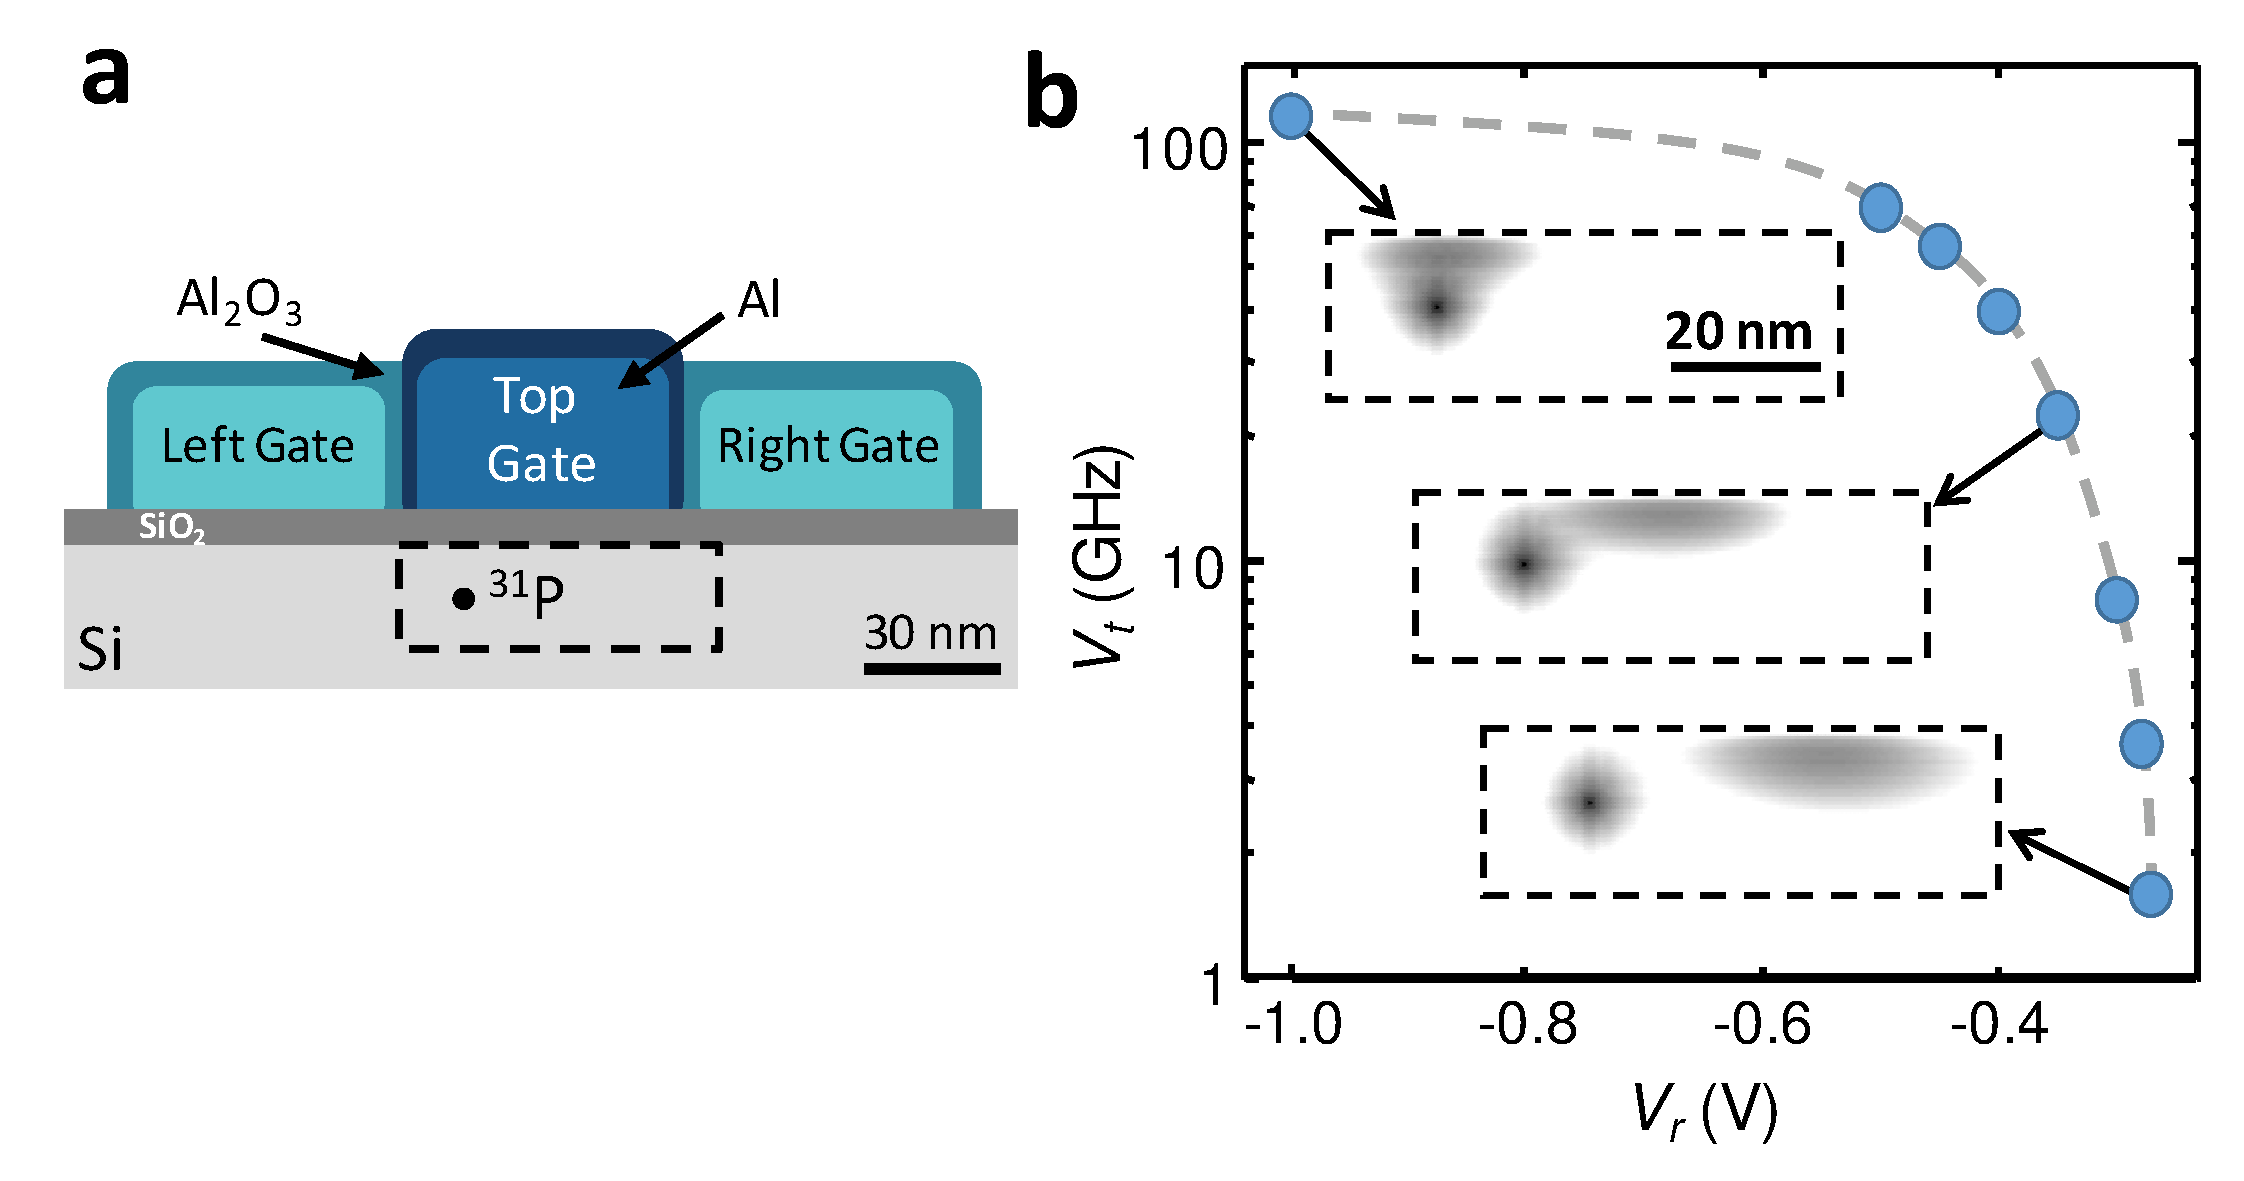
\includegraphics[width=0.8\columnwidth]{polished/Vt_tuning}
	\caption[Tunnel coupling tuning]{\textbf{Tunnel coupling tuning. a} Device structure to tune the tunnel coupling $V_t$ of the charge qubit by applying lateral voltages. 
		\textbf{b}, $V_t$ as a function of right gate voltage, calculated using a finite element Poisson solver (Synopsis\textsuperscript{\textregistered} TCAD) and atomistic tight biding (NEMO-3D, ref.~\cite{Klimeck2007a, Klimeck2007b}). The insets illustrate the NEMO-3D wavefunctions for three right gate voltages $V_r=-1$, $-0.35$ and $-0.27$~V. The left gate voltage is $V_l=-0.5$~V for all the simulations, and the top gate is biased such that the position of the electron is in between the donor and interface. The donor is assumed to be $z_d=9.2$~nm below the Si/SiO$_2$ interface.}
	\label{fig:Vt_tuning}
\end{figure}

This gate stack is identical to the well-established scheme for the confinement of single electrons in Si quantum dots \cite{Veldhorst2014}. This technique allows $V_t$ to be reduced by at least 2 orders of magnitude (Fig.~\ref{fig:Vt_tuning}b), therefore circumventing the uncertainty in donor depth and $V_t$ arising from ion-implantation.

Note that, when moving the interface wavefunction laterally to tune $V_t$, the electric dipole acquires some horizontal component. In this case, the detuning noise is caused by the noise component along the donor-interface states direction. 

\subsection{Adiabatic phase control} \label{sec:adiabatic_pc}

To incorporate flip-flop qubits in a quantum processor, the presence of slow dephasing regions is important to control the qubit phase with high fidelity and extend the qubit lifetime. Therefore, idle qubits are decoupled from electric fields by fully displacing the electron either to the interface or to the donor to minimize dephasing. Operations are performed close to the ionization point. 
Consequently, we need to displace the electron, which in turn changes its precession frequency (Fig.~\ref{fig:ff_energy}). As a result, the accumulated phase must be corrected after quantum operations. This is optimally done by moving the electron to the $2^{\rm nd}$-order clock transition, therefore minimizing dephasing errors. At this point, the flip-flop qubit phase precesses $\sim\Delta_\gamma\gamma_e B_0/2-D_{\rm orb}\sim\ $GHz faster than its idle point, and therefore any phase correction in a $2\pi$ period can be applied within tens of ns. The dephasing rate at the clock transition, on the order of a few kHz, would cause very small errors ($<10^{-4}$). However, while moving the electron from the interface towards the donor, the flip-flop qubit goes through regions of fast dephasing (Fig.~\ref{fig:ff_dephasing}), and therefore this operation has to be performed as quickly as possible. It also has to be slow enough as to avoid erros due to non-adiabaticity, which include \textit{e.g.} leakage to unwanted high-energy states. These errors depend on the adiabatic factor $K$, which quantifies the fractional rate of change of the system's eigenstates (the higher the value of $K$, the more adiabatic and slower is the process). $K$ is defined, in units of rad/s, as

\begin{equation} \label{eq:K_def}
K=\left|\frac{\omega_{\rm eff}}{\dot{\alpha}}\right|\gg1,
\end{equation}

given a time-dependent Hamiltonian in a two-dimensional Hilbert space, 

 \begin{equation}
\mathcal{H}_2=\Delta(t)\sigma_z+\Omega(t)\sigma_x,
\end{equation}

where $\omega_{\rm eff}=\sqrt{\Delta^2+\Omega^2}$ is the instantaneous transition angular frequency between eigenstates, and $\dot{\alpha}$ is the rate of change of the orientation of $\omega_{\rm eff}$ ($\alpha=\arctan{(\Omega/\Delta)}$) \cite{Garwood2001}. 

It follows from Eq.~\ref{eq:K_def} that

\begin{equation} \label{eq:K_appl}
K=\frac{\left(\Delta^2+\Omega^2\right)^{3/2}}{|\dot{\Delta}\Omega-\dot{\Omega}\Delta|}\gg1,
\end{equation}

We use eq. \eqref{eq:K_appl} to determine the incremental sweep time step that satisfies the adiabatic condition at any given point in $E_z$

\begin{equation} \label{eq:dtK}
dt=K\frac{|d\Delta\cdot\Omega-d\Omega\cdot\Delta|}{\left(\Delta^2+\Omega^2\right)^{3/2}}
\end{equation}

where $d\#$ signifies incremental steps in $E_z$.
Although the transition process involves multiple levels, we apply Eq.~\ref{eq:K_appl} as an approximation of adiabaticity. This is confirmed to be always valid by checking that the leakage errors are kept below a target level.
We use $\Delta_{\rm c}=\pi e(E_z - E_z^0)d/h$ and $\Omega_{\rm c}=\pi V_t$ to find $dt_{\rm c}$ for the charge qubit, and $\Delta_{\rm so}=\pi\delta_{\rm so}$ and $\Omega_{\rm so}=2\pi g_{\rm so}$ to find $dt_{\rm so}$ for the spin-charge coupling.
 For a chosen adiabatic factor $K$, we then find $E_z(t)$ by satisfying the condition $\max(dt_{\rm so},dt_{\rm c})=dt$. 

\begin{figure}[h]
	\centering
	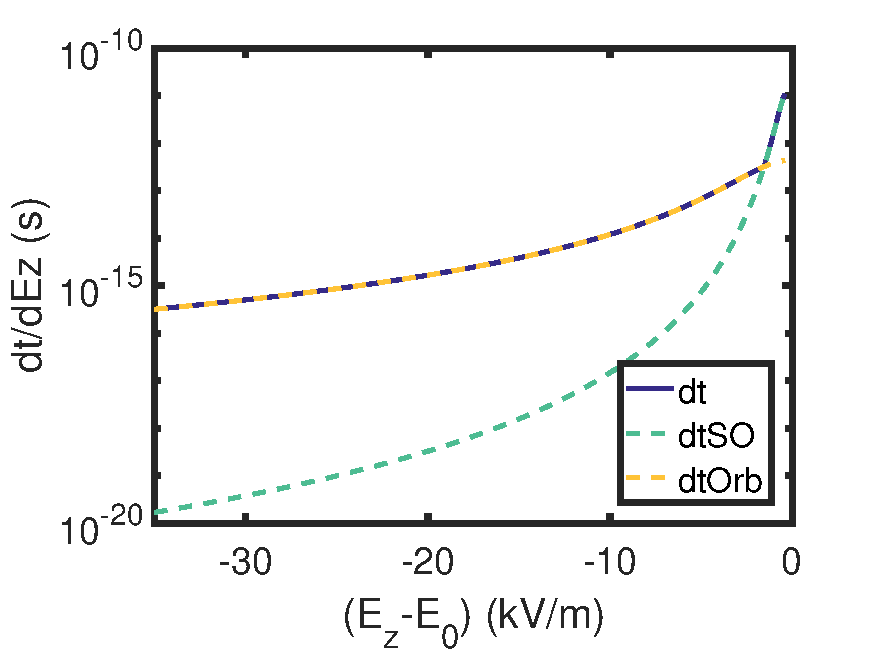
\includegraphics[width=0.8\columnwidth]{polished/adiabatic.pdf}
	\caption[Z-gate adiabaticity time step for each electric field $E_z$]{\textbf{Z-gate adiabaticity time step for each electric field $E_z$}. Time step for each electric field $E_z$ that full fills the adiabaticity criterion from eq. \eqref{eq:K_appl}.}
		\label{fig:adiabatic_dt}
\end{figure}

\begin{figure}[h]
	\centering
	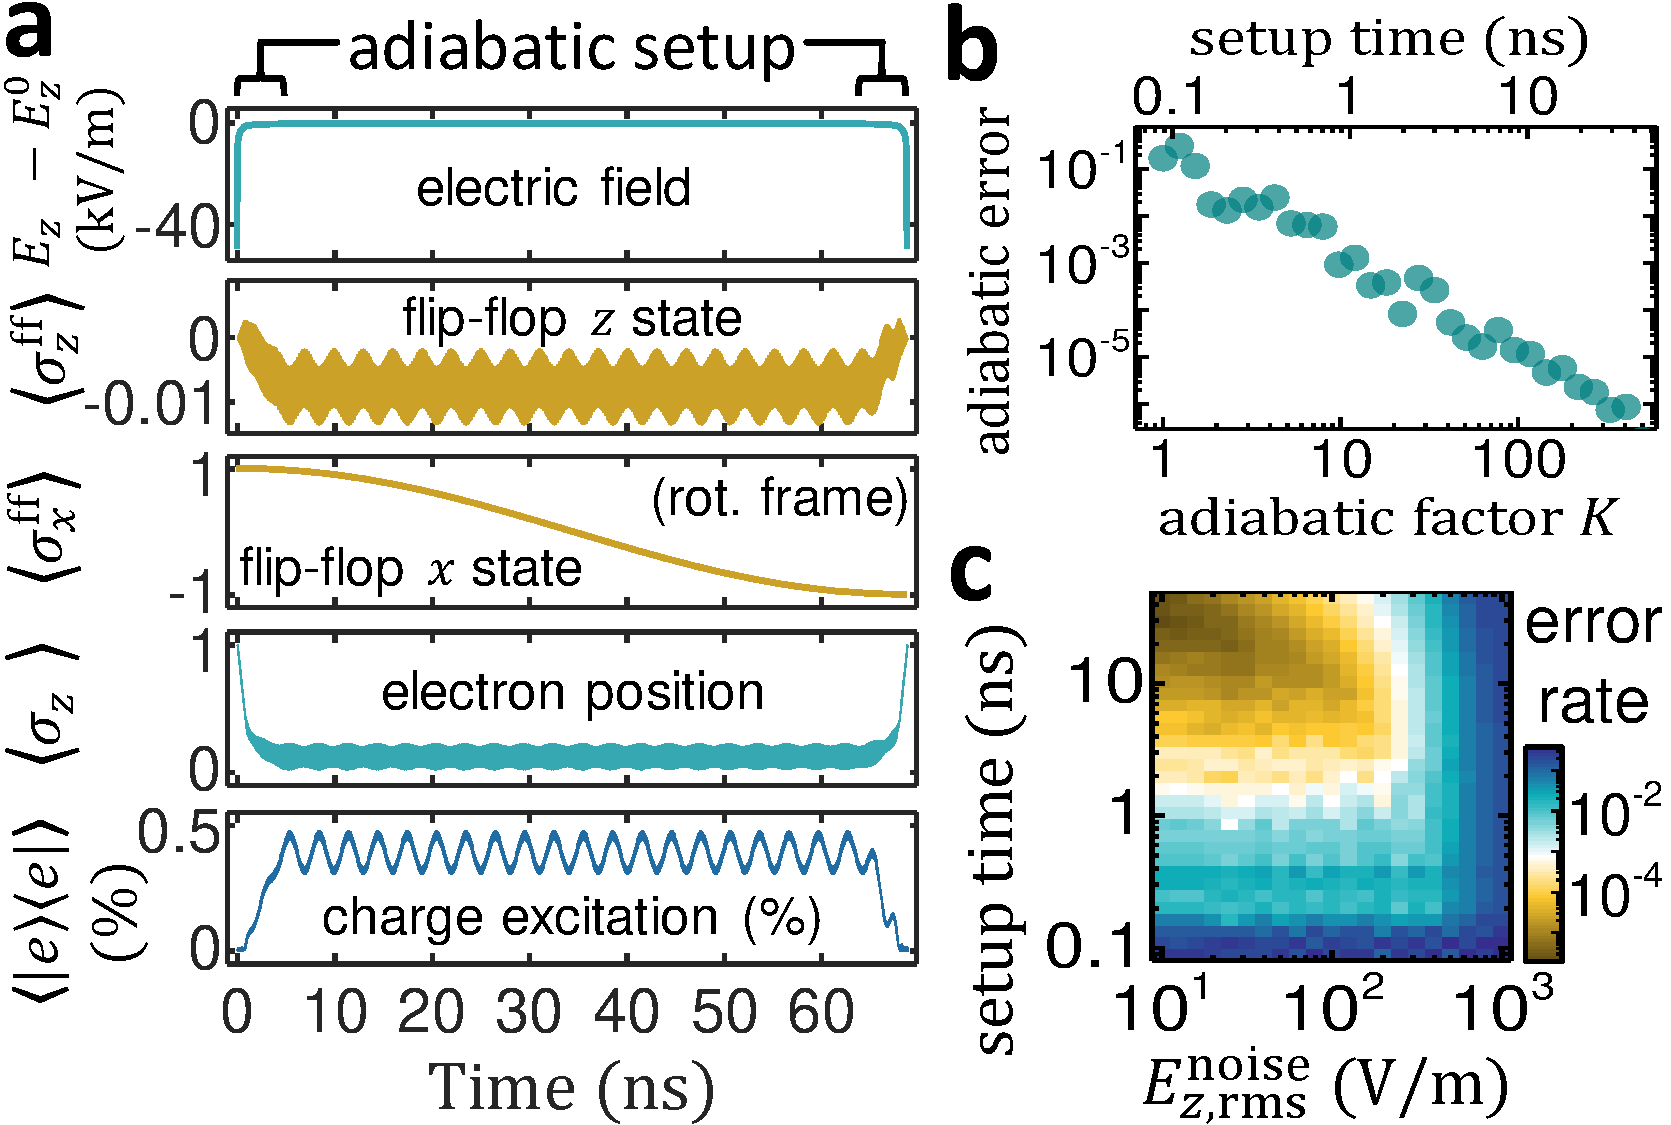
\includegraphics[width=0.9\columnwidth]{polished/z-gate.pdf}
	\caption[High-fidelity adiabatic $z$-gates]{\textbf{High-fidelity adiabatic $z$-gates}.
		\textbf{a}, Time-evolution of an adiabatic  ($K=50$) $\pi$ $z$-gate on state $\ket{g}\otimes(\ket{\downarrow\Uparrow}+\ket{\uparrow\Downarrow})/\sqrt{2}$, showing applied electric field and flip-flop/charge states. Outer brackets denote the expectation value of an operator. $\sigma_z^{\rm ff}=\ket{\uparrow\Downarrow}\bra{\uparrow\Downarrow}-\ket{\downarrow\Uparrow}\bra{\downarrow\Uparrow}$ and $\sigma_x^{\rm ff}=\ket{+_x^{\rm ff}}\bra{+_x^{\rm ff}}-\ket{-_x^{\rm ff}}\bra{-_x^{\rm ff}}$, where $\ket{+_x^{\rm ff}}=\left(\ket{\uparrow\Downarrow}+\exp{\left(-i2\pi\epsilon_{\rm ff}^{t=0}\right)}\ket{\downarrow\Uparrow}\right)/\sqrt{2}$ and $\ket{-_x^{\rm ff}}=\left(\ket{\uparrow\Downarrow}+\exp{\left(-i2\pi\epsilon_{\rm ff}^{t=0}-i\pi\right)}\ket{\downarrow\Uparrow}\right)/\sqrt{2}$. 
		\textbf{b}, $\pi$ $z$-gate leakage error for different adiabatic setup times, which are set by the factor $K$.
		\textbf{c}, $\pi$ $z$-gate error due to quasi-static $E_z$ noise, at the $2^{\rm nd}$-order CT at $B_0=0.4$~T, for different noise amplitudes and adiabatic setup times.}
	\label{fig:z-gate}
\end{figure}

In Fig.~\ref{fig:z-gate}a we plot the time dynamics of an initial state $\ket{g}\otimes(\ket{\downarrow\Uparrow}+\ket{\uparrow\Downarrow})/\sqrt{2}$ while sweeping $E_z$ adiabatically to move the electron from the interface to the $2^{\rm nd}$-order clock transition and back, in order to realize a $\pi$ $z$-gate. Setting $K=50$ eq. \eqref{eq:dtK} gives time steps as shown in Figure \ref{fig:adiabatic_dt}. This results in an initial adiabatic setup consisting of a fast sweep (0.8~ns), allowed by the large charge qubit splitting when $E_z \gg E_z^0$, followed by a slower sweep (3.5~ns), limited by the proximity of excited charge states to the flip-flop qubit when $E_z \approx E_z^0$. The electron then remains at the clock transition for 60~ns to perform the gate to correct for the phase shift, according to 
\begin{equation}
t_{\pi}=\frac{\texttt{gate}/2\pi-\int_{t_0}^{t_{end}} \nu(E_z(t))-\nu(E_z(t_0))dt}{\nu (E_z(t_{end}))-\nu(E_z(t_0))}
\end{equation} 
where gate$=\pi$ and $t_{\rm end}=4.3\,$ns. Afterwards we move it adiabatically back to the interface. We calculate the expectation values for the flip-flop z-state $\langle \sigma_z^{\rm ff}\rangle$, the flip-flop x-state $\langle \sigma_x^{\rm ff}\rangle=\ket{+_x^{\rm ff}}\bra{+_x^{\rm ff}}-\ket{-_x^{\rm ff}}\bra{-_x^{\rm ff}}$, where $\ket{+_x^{\rm ff}}=\left(\ket{\uparrow\Downarrow}+\exp{\left(-i2\pi\epsilon_{\rm ff}^{t=0}\right)}\ket{\downarrow\Uparrow}\right)/\sqrt{2}$ and $\ket{-_x^{\rm ff}}=\left(\ket{\uparrow\Downarrow}+\exp{\left(-i2\pi\epsilon_{\rm ff}^{t=0}-i\pi\right)}\ket{\downarrow\Uparrow}\right)/\sqrt{2}$, the electron position $\langle \sigma_z\rangle$ and the charge qubit excitation $\langle \ket{e}\bra{e}\rangle$ by determining the time evolved eigenstates of our system Hamiltonian 

\begin{equation}
\ket{\psi(t)}=e^{-i \mathcal{H}_{\rm ff} t/\hbar}\ket{\psi(t_0)}
\end{equation}

where $\langle \#\rangle=\bra{\psi(t)}\#\ket{\psi(t)}$ as the expectation value. Indeed during the 69~ns the flip-flop phase $\pi$-gate is performed while keeping both the flip-flop and charge excitation minimal. Fast oscillations between the charge and flip-flop states are due to small deviations from perfect adiabaticity. 

The adiabatic errors (without noise) of an adiabatic unitary process $U_{\rm ideal}$, expressing leakage to other states, can be calculated by averaging the fidelity of the actual process $U$ over a set of initial states $\ket{j}$,

\begin{equation}\label{eq:adError}
{\rm Adiabatic~error}=1-\sum\limits_{\ket{j}}{\left|\bra{j}U^\dagger U_{\rm ideal}\ket{j}\right|^2/N_j},
\end{equation}

where $N_j$ is the number of initial states. For this 1-qubit gate, we choose $\ket{j}=\{\ket{g\downarrow\Uparrow}_e,\ket{g\uparrow\Downarrow}_e,(\ket{g\downarrow\Uparrow}_e+\ket{g\uparrow\Downarrow}_e)/\sqrt{2},(\ket{g\downarrow\Uparrow}_e+i\ket{g\uparrow\Downarrow}_e)/\sqrt{2}\}$ and $N_j=4$. 

These errors can be controlled with the factor $K$, which determines the setup time (see Fig.~\ref{fig:z-gate}b).

Quasi-static $E_z$ noise can increase errors, due to dephasing (Fig. \ref{fig:z-gate}c). At realistic noise levels (100~V~m$^{-1}$), the gate error rate is found to be $<10^{-4}$. Similar error levels arise due to relaxation, which remains below $3\cdot 10^4$~Hz (Fig.~\ref{fig:T1}).\\

Note that the presence of clock transitions does not affect the ability to use $E_{\rm ac}$ to resonantly drive the qubit, since the transverse term $A(E_z)$ still responds fully to the electric field (this is similar to the case of magnetic clock transitions, e.g. in Si:Bi \cite{Wolfowicz2013}).


\section{Electric drive} \label{sec:elecDrive}

\begin{figure}[h]
	\centering
	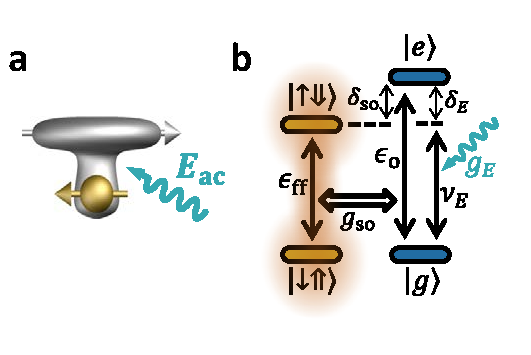
\includegraphics[width=0.7\columnwidth]{polished/elecDrive.pdf}
	\caption[Electric drive of the flip-flop qubit]{\textbf{Electric drive of the flip-flop qubit. a}, Spatial representation and \textbf{b}, level diagram, for electrical drive of a flip-flop qubit, showing partially ionized electron wavefunction and spin arrows.}
		\label{fig:elec_drive}
\end{figure}


We can achieve high-fidelity one-qubit $x(y)$-gates with an electric drive of the flip-flop qubit as illustrated in figure \ref{fig:elec_drive}a.  The fastest 1-qubit gates are obtained when the electron is around the ionization point, where $\partial A/\partial E_z$ is maximum (Fig. \ref{fig:hfchange}). A vertical oscillating electric field of amplitude $E_{\rm ac}$ is applied in resonance with the flip-flop qubit, \textit{i.e}, $\nu_E=\epsilon_{\rm ff}$. This renders $\mathcal{H}_A(t)$ time-dependent. The electric drive is described by the Hamiltonian 

\begin{equation}
H_{\rm E}=E_{\rm ac}\cos(2\pi\nu_E t)\sigma_z.
\end{equation}
The coupling of this electric field to the charge qubit is then determined by 

\begin{eqnarray} \label{eq:g_E}
g_{\rm E}& =& \bra{g}\mathcal{H}_{\rm E}\ket{e}\\
 &=& \frac{e E_{\rm ac} d}{4h}\bra{g}\sigma_z\ket{e}\\
 & = &\frac{e E_{\rm ac} d}{4h}\frac{V_t}{\epsilon_{\rm o}}.
\end{eqnarray}

with eq. \eqref{eq:g_so}. 

This coupling rate corresponds to half the Rabi frequency in the one-photon limit. Furthermore, in every case of resonant driving we assume a linearly polarized field, resulting in a Rabi frequency that equals half the dipole matrix element times the driving field amplitude (rotating-wave approximation, compare chapter \ref{sec:nuchybrid} , eq. \eqref{eq:H_nsRot}). This explains the factors of 4 appearing in all the formulas for coupling rates of driving fields.

Figure \ref{fig:elec_drive}b portraits the energy level diagram for the electric drive.  A large detuning $\delta_{\rm so}\gg g_{\rm so}$ between the charge and flip-flop qubit ensures the least amount of the charge excited state $\ket{e}$ in the flip-flop qubit eigenstates, minimizing qubit relaxation via charge-phonon coupling. The flip-flop qubit is still driven, via a second-order process, at a rate given by second order perturbation theory to:
 
 \begin{equation}
 \label{eq:g_E_ff}
 \begin{aligned} 
g^{\rm ff}_{E}&=\frac{\left| \langle \uparrow\Downarrow g|\mathcal{H}_{\rm ff}\ket{e\downarrow\Uparrow}\langle e\downarrow\Uparrow|\mathcal{H}_{\rm ff}\ket{g\uparrow\Downarrow}\right|}{E_{e\downarrow\Uparrow}-E_{g\uparrow\Downarrow}} ???? \\
&=\frac{g_{\rm so}g_{E}}{2}\left(\frac{1}{\delta_{\rm so}}+\frac{1}{\delta_E}\right),
\end{aligned}
\end{equation}


where $\delta_E=\nu_E-\epsilon_{\rm o}$.
Equation \ref{eq:g_E_ff} provides another explanation of why the fastest 1-qubit gates are obtained when the electron is at the ionization point: $\delta_{\rm so}$ and $\delta_E$ are minimum ($\epsilon_{\rm o}$ is minimum), and $g_{\rm so}$ and $g_E$ are maximum (Eqs. \ref{eq:g_so} and \ref{eq:g_E}).

\begin{figure}[h]
	\centering
	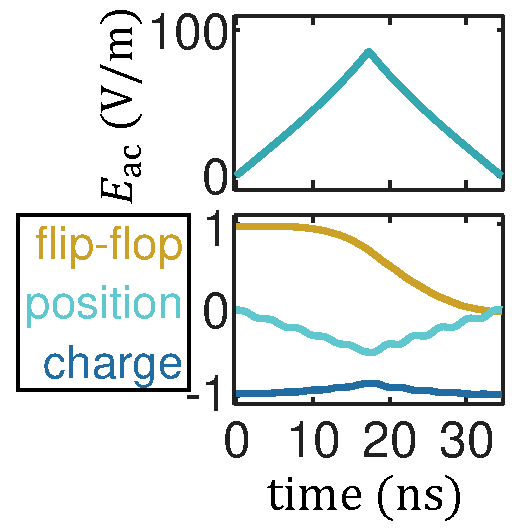
\includegraphics[width=0.4\columnwidth]{polished/adiabaticEdrive.pdf}
	\caption[Adiabatic flip-flop electric drive]{\textbf{Adiabatic flip-flop electric drive} Time-dependent adiabatic drive amplitude and qubit dynamics of a $\pi/2$ $x$-gate, for $K=30$, $B_0=0.4$~T, $E_z=E_z^0$ and $V_t=11.5$~GHz. Bottom plot shows flip-flop z state, $\langle\sigma_z^{\rm ff}\rangle$, electron position, $\langle\sigma_z\rangle$, and charge qubit state, $\langle\ket{e}\bra{e}-\ket{g}\bra{g}\rangle$.}
		\label{fig:adEdrive}
\end{figure}

The electrical drive can cause some excitation of the charge qubit. It is therefore convenient to turn $E_{\rm ac}$ on/off adiabatically to make sure the charge is de-excited at the end of the gate. Figure \ref{fig:adEdrive} shows the $E_{\rm ac}$ time evolution needed for a $\pi/2$ $x$-gate. The adiabatic increase of $E_{\rm ac}(t)$ is calculated with eq. \eqref{eq:K_appl} with $\Delta_E=\pi\delta_E$ and $\Omega_{E}=2\pi g_E$ where we have assumed an adiabatic factor $K=30$, sufficient for leakage errors $<10^{-3}$. Once $E_{\rm ac}(t)$ has been determined, we employ Floquet theory to efficiently calculate the time evolution of the Hamilonian which now changes with every time step.  

Floquet theory says that semi-classical theory provides results that are equivalent to full quantum theory in cases of driving fields interacting with a (qubit) system when fluctuations in the phonon number can be neglected \cite{Chicone1999}. For a periodic Hamiltonian $\mathcal{H}(t)=\mathcal{H}(t+T)$ with period $T$ we define the time propagator as 

\begin{equation}
\ket{\psi(t)}=K(t,t_0)\ket{\psi(t_0)},
\end{equation}
with $K(t_0,t_0)=1$. We can use the propagator over a full period $K(T,0)$ to construct a time evolution over many multiples $n$ of the fundamental period
\begin{equation}
K(nT,0)=[K(T,0)]^n
\end{equation}

This effectively renders our time-dependent Hamiltonian time-independent. We de-construct the adiabatic evolution into a few coarse time steps to account for ?? and thus arrive at the final time-evolved operator $\mathcal{H}$. Then we can calculate the expectation values of flip-flop z-state $\langle \sigma_z^{\rm ff}\rangle$, the electron position $\langle \sigma_z\rangle$ and the charge qubit state $\langle \ket{e}\bra{e}-\ket{g}\bra{g}\rangle$. 
In our $\pi/2$ $x$-gate, $E_{\rm ac}$ increases steadily until a $\pi/4$ rotation is completed, after which $E_{\rm ac}$ is gradually switched off to achieve the gate. Meanwhile, an average 4\% excitation of the charge qubit causes a $\sim4\cdot 10^4$~Hz relaxation rate of the encoded quantum state (Eq. \ref{eq:T1o}), or error levels close to $10^{-3}$. 

\begin{figure}[h]
	\centering
	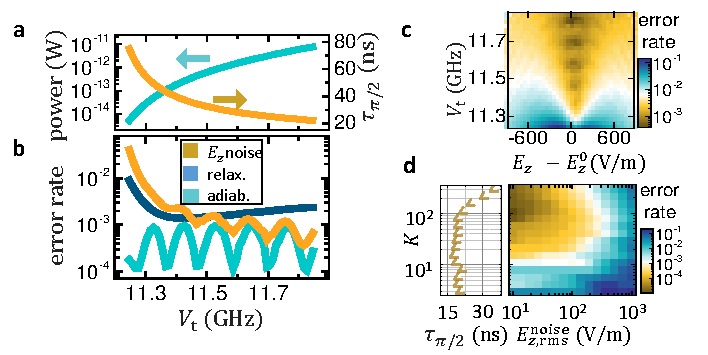
\includegraphics[width=1\columnwidth]{polished/adiabaticError.pdf}
	\caption[Adiabatic gate errors]{\textbf{Adiabatic gate errors. a} Averaged drive power and gate time for the parameters $K=30$, $B_0=0.4$~T, $E_z=E_z^0$ and $V_t=11.5$~GHz. For the same parameters, \textbf{b} the error rates for different $V_t$. To estimate the drive power, we assumed a 50~$\Omega$ line in which a $1~{ \mu \rm V}$ AC voltage produces a 10~V~m$^{-1}$ AC vertical electric field.
		\textbf{c}, Estimated flip-flop qubit $\pi/2$ $x$-gate error due to quasi-static noise with amplitude $E_{z, \rm rms}^{\rm noise}=100$~V~m$^{-1}$.
		\textbf{d}, Dependence of the gate error rate on the electric noise r.m.s. amplitude and adiabatic factor K (which sets the gate time).}
	\label{fig:adError}
\end{figure}

Now we investigate in figure \ref{fig:adError}b how the total $\pi/2$ $x$-gate errors depend on the biasing of the electron wavefunction by calculating the adiabatic error from eq. \eqref{eq:adError} , the error from quasi-static $E_z$ noise from
 
\begin{equation}\label{eq:noiseError}
{\rm Noise~error}=1-\sum\limits_{n,\ket{j}_n}{\left|\bra{j}_nU_n^\dagger U_{n,\rm ideal}\ket{j}_n\right|^2/(N_jN_n)}
\end{equation}
where $\ket{j}=\{\ket{g\downarrow\Uparrow}_e,\ket{g\uparrow\Downarrow}_e,(\ket{g\downarrow\Uparrow}_e+\ket{g\uparrow\Downarrow}_e)/\sqrt{2},(\ket{g\downarrow\Uparrow}_e+i\ket{g\uparrow\Downarrow}_e)/\sqrt{2}\}$ and $N_j=4$
and the relaxation errors from 

\begin{equation}\label{eq:relaxError}
{\rm Relax.~error}=\frac{1-e^{-\int\limits_{0}^{\tau_{\rm gate}}\left({\sum\limits_{\ket{j(t)}}{\braket{j(t)|e}\braket{e|j(t)}/N_j
}}\right)dt/T_{1, \rm c}}}{2},
\end{equation}
where $\ket{j(t)}$ are the time-evolution of the initial set states $\ket{j}$. 

%1. Find adiabatic shape Eac(t)
%2. find time evolved H(t) with Eac(t) through Floquet
%3. Find time evolved states psi with H(t)
%4. Find fideilities with H(t) and Psi(t)

 At the ionization point, $E_z=E_z^0$, error levels close to $10^{-3}$ are found over a wide range of $V_t$. The $K=30$ choice ensures adiabatic errors $<10^{-3}$ with an oscillatory character typical of adiabatic processes \cite{Oh2013}. At small $V_t$ (and therefore small detuning $\delta_{\rm so}$), the qubit eigenstates contain a substantial amount of charge, causing more errors due to charge-phonon relaxation. Increasing the detuning $\delta_E$ with larger $V_t$ allows for a faster adiabatic sweep and higher powers (Fig.~\ref{fig:adError}a), yielding shorter gate times and therefore less errors due to quasi-static noise. Still, the incident power is at least three orders of magnitude lower than the one needed to drive donor electron spin qubits, at the same Rabi frequency, with oscillating magnetic fields \cite{Pla2012,Muhonen2014}.

As Fig. \ref{fig:adError}c shows, low error rates for quasi-static noise (eq. \eqref{eq:noiseError}) are still available away from the ionization point, even though the best values are found at $E_z=E_z^0$. This is because our gate times are so fast that dephasing, and therefore CT's, do not play a crucial role. Instead, quasi-static $E_z$ noise causes errors mainly by modulating the driving strength $g_E^{\rm ff}$, causing ``gate time jitter''. Indeed, the gate time is sensitive to the orbital transition frequency $\epsilon_{\rm o}$ (Eq. \ref{eq:g_E_ff}), and therefore gate errors are minimized close to the charge qubit sweet spot (CQSS), where $\partial\epsilon_{\rm o}/\partial E_z=0$ (Fig. \ref{fig:ff_dephasing}).

Finally, as Fig. \ref{fig:adError}d shows, lower quasi-static $E_z$ noise can cause less errors, provided that the adiabatic factor $K$ is increased, to reduce leakage errors, up to an optimum value where gate times are still fast as to keep noise errors low. Relaxation errors could also be reduced by reducing $B_0$ (recall Fig.~\ref{fig:T1}).

\subsection{Gate noise} \label{sec:gatenoise}
Besides quasi-static $E_z$ noise, a number of other noise sources can also affect the qubits. Another source of electric field noise can be the thermal and electrical noise produced by the metallic gates on top of the qubits, and the room-temperature instruments they connect to. An $R=50~\Omega$ resistor at room temperature produces Johnson-Nyquist noise with an r.m.s voltage $\sqrt{4k_BTR\Delta\nu}$. Therefore a quasi-static bandwidth $\Delta\nu\sim10^6$~Hz produces $\sim1~\mu$V voltage noise, which is equivalent to $E_{z,\rm rms}^{\rm noise}\sim10$~V~m$^{-1}$, or errors $<10^{-5}$ (Fig.~\ref{fig:adError}d). Furthermore, because of the very low powers required by the electrically-driven 1-qubit gates and adiabatic shuttling, it is possible to insert abundant low-temperature attenuation along the high-frequency lines, and therefore the relevant temperature for the Johnson-Nyquist noise is well below room temperature. On the other hand, being close to a metallic interface, our qubit will be subject to evanescent wave Johnson noise (EWJN) due to vacuum and thermal fluctuations (see chapter \ref{sec:ewjn}). Assuming the qubit is $z=15$~nm under aluminum gates at $T=100$~mK ($\sigma=1.6\times10^6$~S~m$^{-1}$ conductivity \cite{Tenberg2018}), a quasi-static bandwidth $\Delta\nu\approx10^6$~Hz produces \cite{Henkel1999} $\sqrt{k_BT\Delta\nu/(2z^3\sigma)}\sim0.01$~V~m$^{-1}$ r.m.s. electric field noise, therefore negligible. We conclude that the main source of quasi-static noise will be charge noise with a typical $1/\nu$ spectrum. Consistently with recently measured for Si/SiO$_2$ interfaces \cite{Freeman2017}, we assume the power spectral density to be $S_{\rm c}(\omega)\approx10^4/(6\omega)$, in units of ${\rm V^2~m^{-2}~rad^{-1}~s}$.

So far we have only considered quasi-static noise. The presence of some residual amount of high-frequency noise could possibly lead to errors while performing quantum operations. Below we discuss these high-frequency sources, finding that they will cause much smaller errors compared to quasi-static noise.

In general, a driven qubit Rabi-oscillates with a decay envelope function given by $\zeta(t)\exp(-\Gamma_Rt)$, \cite{Bylander2011} where $\zeta(t)$ represents decay due to quasi-static detuning noise and $\Gamma_R$ the exponential Rabi decay rate, which combines the qubit relaxation rate, $\Gamma_1$, the inverse of the gate time jitter due to quasi-static noise, $\Gamma_1^{\Delta}$, the inverse of the gate time jitter due to noise at the drive frequency, $\Gamma_1^{\nu}$, (the last three yield $T_{2\rho}$ in the dressed qubit picture \cite{Laucht2016}) and the decay rate due to detuning noise at the Rabi frequency, $\Gamma_\Omega$ (which equals the inverse of $T_{1\rho}$ in the dressed qubit picture \cite{Yan2013,Laucht2016}).

The effects of $\zeta(t)$, $\Gamma_1$ and $\Gamma_1^{\Delta}$ have already been discussed extensively in this chapter, with corresponding error levels below $10^{-3}$. We now focus on errors due to high-frequency noise sources, corresponding to decay rates $\Gamma_1^{\nu}$ and $\Gamma_\Omega$.

Vertical (thus parallel to the driving field $E_{\rm ac}$) noise at the qubit resonance frequency ($\sim 10^{10}$~Hz) would cause transitions between the qubit eigenstates -- essentially a spurious excitation/relaxation process driven by noise -- at a rate $\Gamma_1^{\nu}$. This noise can be caused $e.g.$ by charges fluctuating in resonance with the qubit or by voltage noise at the metallic gates. This includes vacuum fluctuations, especially since the qubit frequency is generally higher than the corresponding device temperature. Also, during gate operations, the portion of the noise spectrum %contained within a power-broadened bandwidth $<10^5$~Hz
around the qubit frequency can add incoherently to the external resonant drive, causing the gate time to fluctuate. For the flip-flop qubit, the Rabi decay rate is given by $\Gamma_1^\nu=(\pi/2)(\mu_e^{\rm ff}/\hbar)^2S(2\pi\epsilon_{\rm ff})$, where $\mu_e^{\rm ff}=ed\langle g_{\rm so}/\delta_{\rm so}\rangle$ is the average flip-flop qubit electric dipole moment and $S(2\pi\epsilon_{\rm ff})$ is the noise power spectral density at the qubit angular frequency (in units of ${\rm V^2~m^{-2}~rad^{-1}~s}$). Note that this flip-flop electric dipole is much smaller than the charge dipole, which in turn makes it less susceptible to electrical noise. This happens because, in our gate scheme, the charge dipole is only used as a second-order enabler, and therefore charge excitation is greatly minimized (Figs. \ref{fig:z-gate}a, \ref{fig:adEdrive} and \ref{fig:iSWAP}a). In case of charge noise, $S_{\rm c}(\omega)=10^4/(6\omega)$ we get $\Gamma_1^\nu\sim10^4$~Hz. This implies $\pi/2$ $x$-gate errors $\sim10^{-4}$. There could also be vacuum fluctuations of charge traps, which could also generate errors due to relaxation. We do not know of any experimental measurement of such a noise for semiconductor nanostructures. For superconducting charge qubits, it has been found that charge noise increases linearly at frequencies beyond the thermal bath \cite{Astafiev2004}, which has been explained in terms of two-level coherent charge fluctuators \cite{Shnirman2005}. If a similar phenomenon afflicts our qubits, those quantum fluctuations will play an important role beyond $\sim2$~GHz (100 mK), implying that, at 10 GHz, relaxation can be up to 25 times faster. This can increase relaxation error rates to $\sim10^{-3}$. In case of Johnson-Nyquist noise we have $S_{\rm JN}(\omega)= 2\times10^{14}R\hbar\omega\pi^{-1}(e^{\hbar\omega/k_BT}-1)^{-1}$ (where we have used $\partial E_z/\partial V=10^7~{\rm m^{-1}}$, typical in MOS nanostructures). Because of the very low powers required by the electrically-driven 1-qubit gates ($<1$~pW), it is possible to insert abundant low-temperature attenuation along the high-frequency lines, insuring that the gates are well thermalized, and the noise of the room-temperature electronics is greatly attenuated. A noise temperature $T=100$~mK would give $\Gamma_1^\nu<10^4$~Hz, and therefore error rates $<10^{-4}$. Finally, in case of EWJN at $T=100$~mK, the $10^{10}$~Hz part of the spectrum is  $S_{\rm EW}(\omega)\approx\hbar\omega/(4\pi z^3\sigma)$, \cite{Henkel1999,Poudel2013}. This would give $\Gamma_1^\nu<10^4$~Hz, therefore again error rates $<10^{-4}$.

Noise at the Rabi frequency ($\Omega_R>10^{7}$~Hz) causes decay in the Rabi oscillations at a rate $\Gamma_\Omega$. This type of noise feeds into the driven qubit via fluctuations in the detuning between drive frequency and the qubit precession frequency. The decay rate of the flip-flop qubit is given by $\Gamma_\Omega=(\pi/2)(2\pi\sum_{i=x,y,z}\partial\epsilon_{\rm ff}/\partial E_i)^2S(\Omega_R)$. At the low-error operation region of Fig. \ref{fig:adError}c, $\partial\epsilon_{\rm ff}/\partial E_z\sim10^3~{\rm Hz~V^{-1}~m}$ and $\partial\epsilon_{\rm ff}/\partial E_{x,y}\sim10^2~{\rm Hz~V^{-1}~m}$ (from Fig.~\ref{fig:Vt_tuning}b). $1/\nu$ charge noise gives $\Gamma_\Omega<10^4$~Hz, implying $<10^{-4}$ errors. Johnson-Nyquist noise from room temperature gives $\Gamma_\Omega=3\times10^2$~Hz, whereas EWJN at 100~mK gives $\Gamma_\Omega=2\times10^1$~Hz, therefore producing $<10^{-5}$ and $<10^{-6}$ errors, respectively.

At the same time, horizontal noise will also have an effect, albeit minimal, in gate performance. For the parameters at which $V_t\approx 10$~GHz in Fig.~\ref{fig:Vt_tuning}b, $10~\mu$V r.m.s. lateral noise would cause less than 0.01\% uncertainty in the dipole size, therefore causing negligible gate errors. The same noise causes less than 1\% uncertainty in $\delta_{\rm so}$ (and therefore in gate time), which translates into maximum $10^{-4}$ errors due to gate time jitter, and maximum $\sim10^4$~Hz extra dephasing due to dispersive shifts (Eq. \ref{eq:Dorb}).


\begin{table}
\centering
\begin{tabular}{|p{1.4in}|p{0.7in}|p{0.7in}|p{0.7in}|} \hline 
 & \multicolumn{3}{|p{2.0in}|}{\textbf{Error levels at different spectral bandwidths}} \\ \hline 
\textbf{Noise source} & Quasi-static\newline ($<$10${}^{6}$ Hz) & Rabi\newline ($\sim 10^{7}$ Hz) & Qubit\newline ($\sim 10^{10}$ Hz) \\ \hline 
1/f vertical ($E_z$) & $10^{-3}$ & $<10^{-4}$ & $10^{-4}$ \\ \hline 
1/f horizontal ($E_{x,y}$) & $10^{-4}$ & $<10^{-5}$ & - \\ \hline 
Charge-phonon\newline relaxation & - & - & $10^{-3}$ \\ \hline 
Johnson-Nyquist & $<<10^{-5}$ & $<10^{-5}$ & $<10^{-4}$ \\ \hline 
EWJN & - & $<10^{-6}$ & $<10^{-4}$  \\ \hline 
\end{tabular}
	\caption[Gate errors for different noise sources]{\textbf{Gate errors for different noise sources} Hyphens indicate non-existent or negligible errors.}
	\label{tab:noise}
\end{table}

We conclude that quasi-static $E_z$ noise and charge-phonon relaxation are the main sources of error and the most deleterious ones for flip-flop qubits. Therefore our analysis is sufficient to provide a reliable estimate of dephasing and gate errors. Indeed, low-frequency noise was found to be the most deleterious one in a hybrid donor-dot qubit in a silicon MOS device \cite{Harvey-Collard2017}. Finally, note that we do not assume any type of dynamical noise correction or cancellation to be applied, and therefore our calculations are a worst-case scenario. Table \ref{tab:noise} summarizes these results. 

\section{Dipole-dipole coupling} \label{sec:dd_coupling}

To couple two flip-flop qubits, we exploit the electric dipole that naturally arises when a donor-electron wavefunction is biased to the ionization point, due to the fact that a negative charge has been partly displaced away from the positive $^{31}$P nucleus. The electric field produced by this induced dipole in turn, modifies the energy of a nearby donor which is also biased at the ionization point, resulting in a long-range coupling between the two. This is illustrated in figure \ref{fig:dipole}a.

\begin{figure}[h]
	\centering
	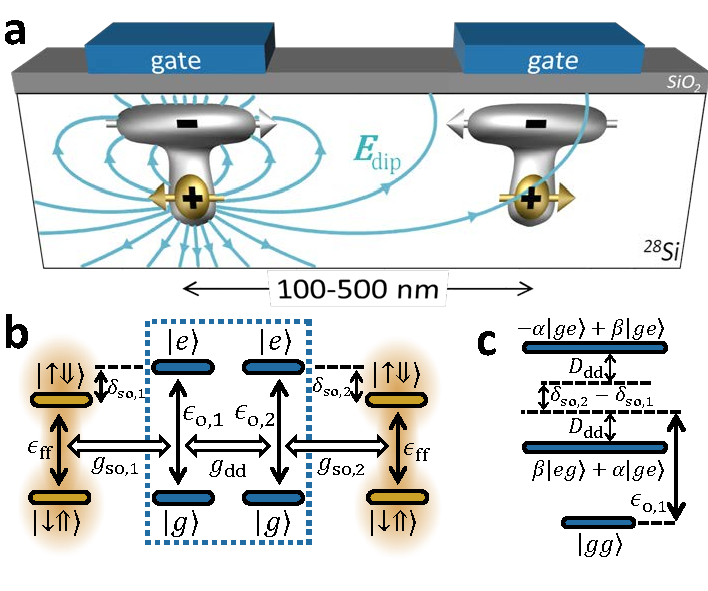
\includegraphics[width=0.8\columnwidth]{polished/2qubit_dipole.pdf}
	\caption[Electric dipole-dipole interactions between two distant flip-flop qubits]{\textbf{Electric dipole-dipole interactions between two distant flip-flop qubits. a}, Device scheme for coupling qubits, showing dipole field lines, $\textit{\textbf{E}}_{\rm dip}$, produced by the dipole on the left.
		\textbf{b}, Level diagram for two-qubit coupling via electric dipole-dipole interaction.
		\textbf{c}, Lowest molecular eigenstates for the two charge qubits inside dashed rectangle in \textbf{b}.}
	\label{fig:dipole}
\end{figure}

The interaction energy between two distant dipoles, $\mu_1$ and $\mu_2$, oriented perpendicularly to their separation $r$ is $V_{\rm dip}=\mu_1\mu_2/(4\pi\varepsilon_r\varepsilon_0r^3)$, where $\varepsilon_0$ is the vacuum permittivity and $\varepsilon_r$ the material's dielectric constant ($\varepsilon_r=11.7$ in silicon)\cite{Ravets2014}. The electric dipole of each donor-interface state is $\mu_i=ed_i(1+\sigma_{z,i})/2$, implying that the dipole-dipole interaction Hamiltonian is:

%\begin{subequations}
\begin{equation} \label{eq:H_dipdip}
\mathcal{H}_{\rm dip}=V_{\rm dd}\left(\sigma_{z,1}\sigma_{z,2}+\sigma_{z,1}+\sigma_{z,2}\right),
\end{equation}
\begin{equation} \label{eq:V_dd}
V_{\rm dd}=\frac{1}{16\pi\varepsilon_0\varepsilon_r h}\frac{e^2d_1 d_2}{r^3}
\end{equation}
%\end{subeq uations}

This electric dipole-dipole interaction is therefore equivalent to a small shift in the equilibrium orbital position of both electrons plus a coupling term between the charge qubits (blue dashed rectangle in Fig. \ref{fig:dipole}b) equal to:

\begin{equation}\label{eq:g_dd}
\begin{aligned} 
g_{\rm dd} & =  \bra{e_1g_2}H_{\rm dip, coupling}\ket{g_1e_2}\\
 & =  V_{dd}\bra{e_1}\sigma_{z,1}\ket{g_1}\bra{g_2}\sigma_{z,2}\ket{e_2}\\
 & =   V_{\rm dd}\frac{V_{t,1}V_{t,2}}{\epsilon_{\rm o,1}\epsilon_{\rm o,2}}
\end{aligned}
\end{equation}

The strength of the dipole interaction is influenced by screening effects due to the dielectric/metal surface above it.    

\subsection{Dipole Screening} \label{sec:screening}

Our device topology consists of a SiO$_2$ layer sandwiched between a metal gate and silicon substrate, with the donor embedded in the substrate. In such a topology, the image charges of the donor electron and nucleus will be located above the donor, thereby creating an additional vertical dipole.

\begin{figure}
\centering
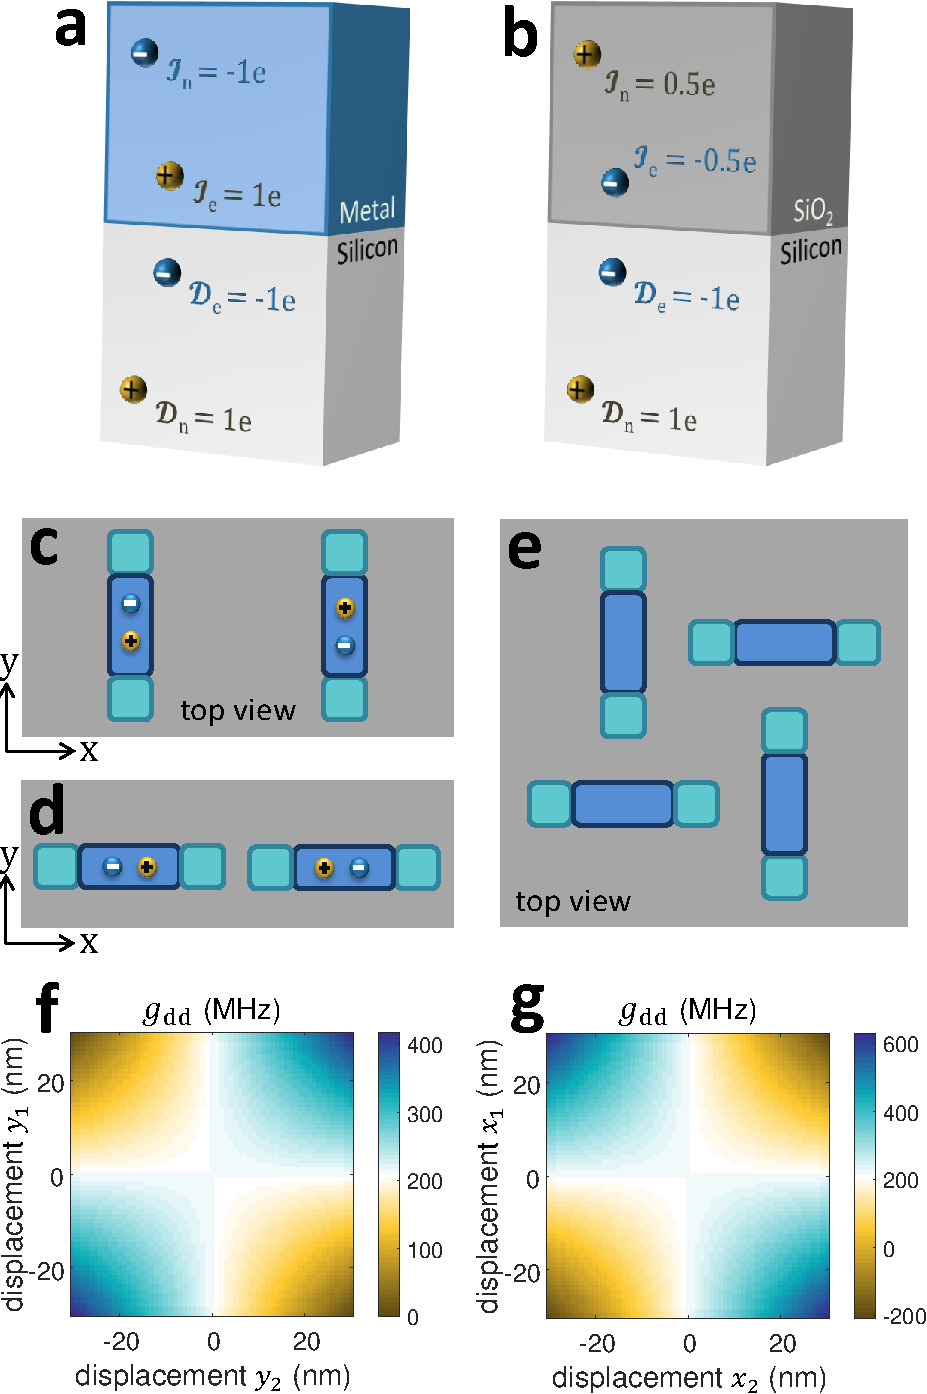
\includegraphics[width=0.7\columnwidth]{polished/image-charges.pdf}
\caption[Screening and image charges]{\textbf{Screening and image charges.} Image ($\mathcal{I}_\mathrm{e}$ and $\mathcal{I}_\mathrm{n}$) charges of the donor electron ($\mathcal{D}_\mathrm{e}$) and nucleus ($\mathcal{D}_\mathrm{n}$) for silicon-metal (\textbf{a}) and silicon-oxide (\textbf{b}) interfaces. The magnitude and polarity of the image charges are given by Eq. \ref{eq:ImageCharge}. Schematic top view of two interacting dipoles when the negative charges (blue spheres) are displaced in perpendicular (\textbf{c}) and parallel (\textbf{d}) direction to the inter-dipole separation. \textbf{e}, Top view of gate stack that tunes each qubit's $V_t$ by displacing their interface states perpendicularly to their nearest neighbor displacement, leaving $g_{\rm dd}$ unchanged. Inter-dipole coupling $g_{\rm dd}$, as predicted by eq. \eqref{eq:g_dd} with eq. \eqref{eq:V_dd_ic}, for the orientation shown in \textbf{c} (\textbf{f}) and \textbf{d} (\textbf{g}), for $r=200$~nm, $d_1=d_2=10$~nm and $Q=-0.5$.}
\label{fig:image_charge}
\end{figure}

The magnitude and polarity of the image charges depend on the details of the nanostructure, such as the donor depth and thickness of the oxide. We first analyze two extreme scenarios considering image charges at (i) silicon-metal and (ii) silicon-oxide interfaces. For a source donor electron (or nuclear) charge $\mathcal{D}_\mathrm{e(n)}$, in silicon, the image charge $\mathcal{I}_\mathrm{e(n)}$ in the interface material is given by\cite{Rahman2009}

%\begin{subequations}
\begin{equation} \label{eq:ImageCharge}
\mathcal{I}_\mathrm{e(n)}=Q~\mathcal{D}_\mathrm{e(n)},
\end{equation}
\begin{equation} \label{eq:Q}
Q=\frac{\epsilon_{\rm Si} - \epsilon_{\rm I}}{\epsilon_{\rm Si} + \epsilon_{\rm I}},
\end{equation}
%\end{subequations}

where $\epsilon_{\rm Si} =$ 11.7 is the dielectric constant of silicon,  $\epsilon_{\rm I} =$ 3.9 and  $\infty$  for oxide and metal interfaces respectively. Figures \ref{fig:image_charge}a,b show the magnitude and polarity of the image charges for both types of interfaces. For simplicity, we assume in Fig. \ref{fig:image_charge} and Eq. \ref{eq:ImageCharge} that the donor electron as well as its image are point charges. Given that the separation between the two donors is at least 180 nm (more than hundred times the Bohr radius of the donor electron), the above assumption is valid when calculating their dipolar interaction. 

We first consider the electric dipole to be vertical. For the silicon-metal interface in Fig. \ref{fig:image_charge}a, $Q=-1$ and therefore the image charges have the opposite sign and same magnitude as the source charges. As a result, the total electric field  $E_{\rm dip}$ from each donor will be enhanced by a factor of 2. This improves the electric dipole coupling $g_{\rm dd}$ between the two donors by a factor of 4. On the contrary, for the silicon-oxide interface in Fig. \ref{fig:image_charge}b, the image charges have the same sign and reduced magnitude ($Q=0.5$) as the source charges, which decreases $E_{\rm dip}$ by half and therefore $g_{\rm dd}$ to a quarter of its bare value.

For a real device, which typically contains a few metal gates on top of a $\sim8$~nm thick SiO$_2$, it is difficult to make a precise estimate of the extra electric field from image charges. Rahman \textit{et. al.} \cite{Rahman2009} assumed that a combination of metallic and oxide screening effects yields $Q=-0.5$, corresponding to an improvement in the magnitude of the electric dipole by $\approx$ 50\%, which yields an improvement in $g_{\rm dd}$ by 125\%. 
This means that, while building a real device, one would have to aim for slightly larger inter-donor separations than the ones presented here.

Since the donor-interface tunnel coupling $V_t$ has to be tuned to a precise value, the dipole will also have lateral components as shown on the insets of Fig.~\ref{fig:Vt_tuning}. These components will also be affected by image charges. In the case of a metallic interface, Fig. \ref{fig:image_charge}a, the lateral image dipole has opposite direction as the original one, and therefore the total lateral component will be completely screened. On the other hand, for the SiO$_2$ interface, Fig. \ref{fig:image_charge}b, the lateral component will be enhanced by 50\%. Finally, for our assumed real structure ($Q=-0.5$), the lateral dipole will decrease to half its original value.

In total, the dipole size and orientation, including screening, will be:

\begin{equation} \label{eq:D_ic}
\textbf{D}_i=\textbf{d}_i+Q\times(d_{i,x},d_{i,y},-d_{i,z}),
\end{equation}

where $\textbf{d}_i$ refers to the bare dipole, with $x$, $y$ and $z$ components $d_{i,x}$, $d_{i,y}$ and $d_{i,z}$, respectively.

As the image charges decrease a lateral dipole, the uncertainty in the total electric dipole of a donor-interface state is minimal, even when displacing the interface wavefunction laterally to tune up $V_t$. At $V_t\approx10$~GHz, the total dipole size of Fig. \ref{fig:nemolevels} ($d_z=11$~nm) is $(1+0.5)d_z=16.5$~nm, while the one of Fig. \ref{fig:Vt_tuning} ($d_z=5$~nm, $d_x=25$~nm) is $\sqrt{[(1+0.5)d_z]^2+[(1-0.5)d_x]^2}=14.6$~nm. This is important for qubit reproducibility over a large scale processor.

To include images charges and angular dependencies, the dipole-dipole interaction term, Eq. \ref{eq:V_dd}, has to be modified to \cite{Ravets2014}:

\begin{equation} \label{eq:V_dd_ic}
V_{\rm dd}=\frac{e^2}{16\pi\varepsilon_0\varepsilon_r h}\frac{\textbf{D}_1\cdot\textbf{D}_2-3(\textbf{D}_1\cdot\textbf{r})(\textbf{D}_2\cdot\textbf{r})/r^2}{r^3},
\end{equation}

We neglect the interaction of a dipole with its own charge since it does not produce inter-donor coupling.

Laterally displacing the interface charge is, in general, necessary for the purpose of tuning the donor-interface tunnel coupling $V_t$. This displacement, however, also alters the total electric dipole direction and can therefore affect the dipole-dipole coupling $g_{dd}$ between neighbouring qubits. We first consider the case in which the displacements are perpendicular to the separation between dipoles,  Fig. \ref{fig:image_charge}c. The $g_{\rm dd}$ dependence on $y_1$ and $y_2$ is plotted in Fig. \ref{fig:image_charge}f, for maximum displacements of 30~nm (enough to tune $V_t$ by two orders of magnitude -- see Fig \ref{fig:Vt_tuning}b). It shows that, provided that the interface states are displaced along the same direction, $g_{\rm dd}$ only varies by a factor of two. For completeness, we also analyze the case in which the interface states are displaced in the same direction as the inter-donor separation (Fig. \ref{fig:image_charge}d). As can be seen in the plot in Fig. \ref{fig:image_charge}g, $g_{\rm dd}$ varies by a factor of three if the interface states are displaced in opposite directions. Finally, the variation in $g_{\rm dd}$ can be reduced even further by fabricating the gate stack in such a way that the charges in neighbouring qubits are displaced in perpendicular directions, as in Fig. \ref{fig:image_charge}e. In this way, from Eq. \ref{eq:V_dd_ic}, the only dipole terms contributing to the coupling are the vertical ones, and therefore $g_{\rm dd}$ is unchanged (to first order) while tuning $V_t$.

\subsection{Two-qubit coupling}
The electric dipole-dipole interaction provides a natural way to couple two distant flip-flop qubits since each flip-flop qubit is coupled to their electron position (Eq.~\ref{eq:H_A}). We compute the 2-qubit coupling strength between the singlet ground state and excited triplet state

\begin{eqnarray}
\ket{S}&=&\frac{1}{\sqrt{2}}\left(\ket{g_1\uparrow_1\Downarrow_1, g_2\downarrow_2\Uparrow_2}-\ket{g_1\downarrow_1\Uparrow_1, g_2 \uparrow_2\Downarrow_1}\right)\\
\ket{T}&=&\frac{1}{\sqrt{2}}\left(\ket{g_1\uparrow_1\Downarrow_1, g_2\downarrow_2\Uparrow_2}+\ket{g_1\downarrow_1\Uparrow_1, g_2 \uparrow_2\Downarrow_1}\right)
\end{eqnarray}
as the corresponding eigenenergy difference with the Hamiltonian
\begin{equation}
\mathcal{H}=\mathcal{H}_{\rm ff}^1+\mathcal{H}_{\rm ff}^2+\mathcal{H}_{\rm dip}.
\end{equation}

\begin{figure}[h]
	\centering
	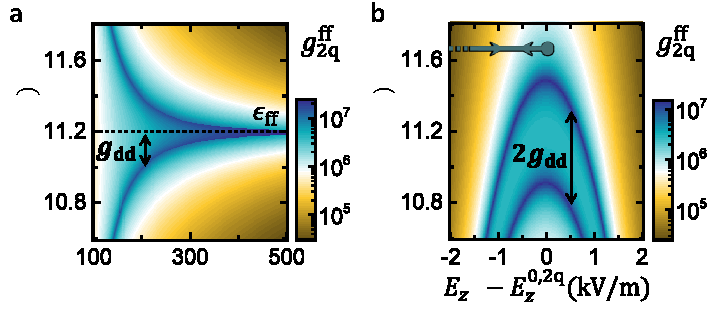
\includegraphics[width=\columnwidth]{polished/2qubit.pdf}
	\caption[Coupling rate between 2 flip-flop qubits]{\textbf{Coupling rate between 2 flip-flop qubits. a}, Effective coupling between 2 flip-flop qubits as a function of $V_{t,1}=V_{t,2}=V_t$, interdistance $r$ (\textbf{a}) and electric field $E_{z,1}=E_{z,2}=E_z$ (\textbf{b}). The arrows in \textbf{b} represent the adiabatic path followed for 2-qubit gates. }
	\label{fig:2-qubit}
\end{figure}

 Figure \ref{fig:2-qubit}a shows the results at the ionization point $E_z^{\rm 0,2q}=E_z^0-2g_{\rm dd}h/(2ed_i)$, which is shifted by the presence of the second qubit, for a range of qubit distances $r$. The coupling rate exceeds $10$~MHz around two narrow regions when the flip flop qubit is in resonance with a molecular state as the two charge qubits in Fig.~\ref{fig:dipole}b form hybridized molecular states, which are coupled to each flip-flop qubit as illustrated in figure \ref{fig:dipole}c. The states of the hybridized molecular states are
 
\begin{eqnarray}
\tilde{g}=\beta\ket{eg}+\alpha\ket{ge}\\
\tilde{e}=-\alpha\ket{eg}+\beta\ket{ge}
\end{eqnarray}

,similar to eq. \eqref{eq:hybridstates}, with the coefficients as in eq. \eqref{eq:ab} and\eqref{eq:abcont} and $A=\delta_{so,2}-\delta_{so,1}$, $B=2g_{dd}$. The coupling between the two charge qubits additionally creates an AC Stark shift of the charge qubit eigenenergies (compare chapter \ref{sec:flipflop}).

The resonant regime, however, induces too many relaxation errors due to resonant charge excitation. Therefore it is best to detune the flip-flop qubits from the molecular states, while still keeping a substantial inter-qubit coupling rate, via a second-order process.
 We calculate this coupling rate between the flip-flop qubits to 
 
 \begin{equation}
 \label{eq:flipdipSWAP_Delta}
 \begin{aligned}
g_{\rm 2q}^{\rm ff} &= \bra{\uparrow_1\Downarrow_1 \downarrow_2\Uparrow_2 \tilde{g}}\mathcal{H}_{\rm tot}\ket{\downarrow_1\Uparrow_1 \uparrow_2\Downarrow_2 \tilde{g}} \\
& = g_{\rm so,1}g_{\rm so,2}\alpha\beta\left(\frac{1}{D_{\rm dd}-\delta_{\rm so,1}}+\frac{1}{D_{\rm dd}+\delta_{\rm so,2}}\right)
\end{aligned}
\end{equation}
where 

\begin{equation}\label{eq:Ddd}
\begin{aligned}
D_{\rm dd}&=\frac{\left| \langle g_1 e_2|\mathcal{H}_{\rm orb}^A+\mathcal{H}_{\rm dip}\ket{e_1 g_2}\langle e_1 g_2 |\mathcal{H}_{\rm orb}^A +\mathcal{H}_{\rm dip}\ket{g_1 e_2 }\right|}{E_{e_1 g_2}-E_{g_1 e_2}}\\
& =  (\delta_{\rm so,2}-\delta_{\rm so,1})\left(1+[2g_{\rm dd}/(\delta_{\rm so,2}-\delta_{\rm so,1})]^2\right)/2
\end{aligned}
\end{equation}

 is the charge eigenenergy shift.

Figure \ref{fig:2-qubit}b shows the coupling rate as a function of electric field at a fixed inter-qubit distance of $r=180\,$nm. 


\subsection{Two-qubit gates} \label{sec:2q_gates}

2-qubit gates start with both electrons at the interface, where qubits are decoupled since the electric dipoles and the hyperfine interactions are first-order insensitive to vertical electric fields. Indeed, from Eq.~\ref{eq:flipdipSWAP_Delta}, $g_{\rm 2q}^{\rm ff}$ is negligible since $g_{\rm so}$ vanishes and $\delta_{\rm so}$ diverges. The electrons are then simultaneously and adiabatically displaced to the ionization point for a time necessary for an $\sqrt{i\mathrm{SWAP}}$ gate, before returning to the interface. 

\begin{figure}[h]
	\centering
	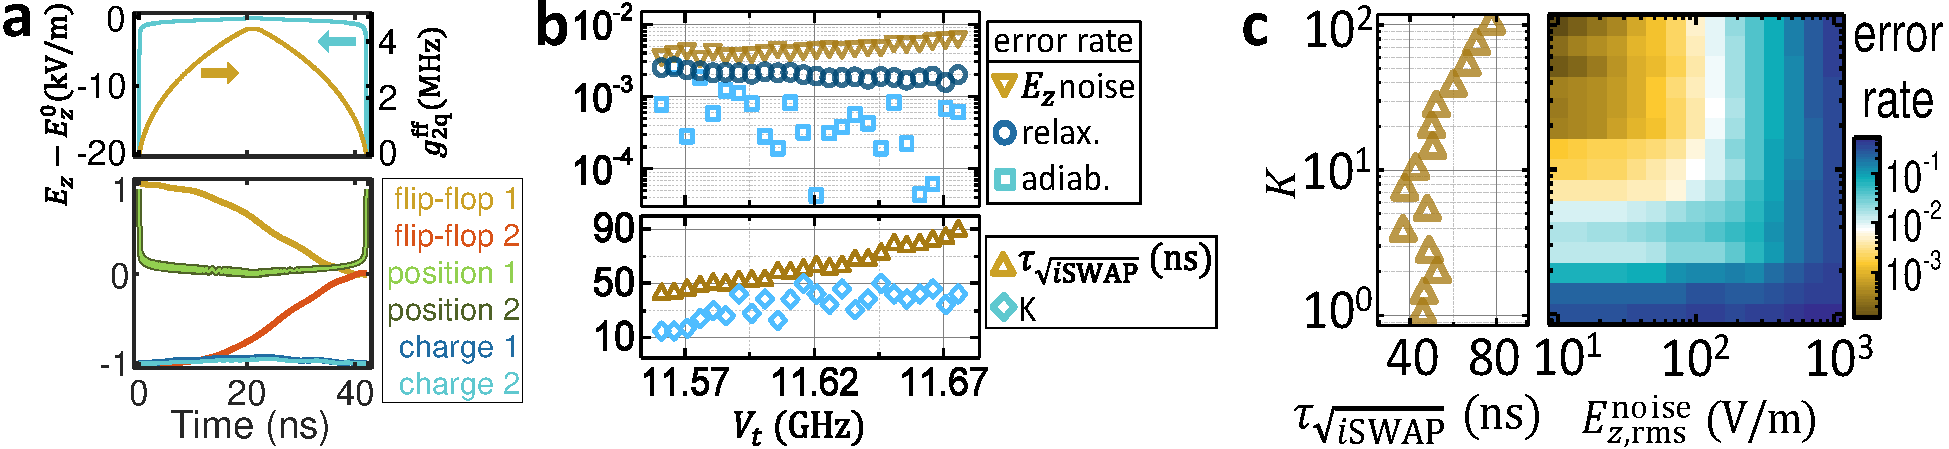
\includegraphics[width=1\columnwidth]{polished/iSWAP.pdf}
	\caption[High-fidelity adiabatic $\sqrt{i{\rm SWAP}}$ gates between two distant flip-flop qubits]{\textbf{High-fidelity adiabatic $\sqrt{i{\rm SWAP}}$ gates between two distant flip-flop qubits.}
		\textbf{a}, Time evolution of an adiabatic $\sqrt{i \rm SWAP}$ gate, for $K=30$, $r=180$~nm, $B_0=0.4$~T and $V_t=11.58$~GHz.
		\textbf{b}, Optimized $\sqrt{i{\rm SWAP}}$ gate error, gate time and adiabatic factor $K$.
		\textbf{c}, Optimized error rate arising from quasi-static $E_z$-noise, for different noise amplitudes and adiabatic factor $K$ (which sets the gate time).}
	\label{fig:iSWAP}
\end{figure}


In Fig.~\ref{fig:iSWAP}a we show the dynamics of a 2-qubit gate performed with an adiabatic factor $K=30$, following the trajectory shown in Fig.~\ref{fig:2-qubit}b. Similarly to 1-qubit $z$ gates (compare chapter \ref{sec:adiabatic_pc}), the electron is first displaced in a fast time scale ($\sim0.3$~ns) set by the charge qubit parameters ($\epsilon_{\rm o}$ and $V_t$), followed by a slower sweep ($\sim19$~ns) set by the spin-charge coupling parameters ($\delta_{\rm so}$ and $g_{\rm so}$), until it reaches the ionization point. The electron remains still for a short time before the whole process is then reversed. In the end a $\sqrt{i\mathrm{SWAP}}$ gate is performed. While some amount of charge is excited during the process, it goes back to its ground state, $\ket{gg}$, with an adiabatic error around $10^{-3}$.

We quantify the 2-qubit gate fidelity in presence of the most deleterious noise types for our qubits, namely quasi-static $E_z$ noise and charge-phonon relaxation. For this, we observe that the optimal gate fidelities are achieved when $E_z(\tau_{\sqrt{i\mathrm{SWAP}}}/2)\approx E_z^0$. Similarly to 1-qubit $x$-gates, this happens because $\sqrt{i\mathrm{SWAP}}$ gates are sensitive to gate time jitter, and therefore errors are minimized at the CQSS where $g_{\rm 2q}^{\rm ff}$ is robust against $E_z$ noise to first order -- recall Fig.~\ref{fig:2-qubit}b and Eq.~\ref{eq:flipdipSWAP_Delta}). We find the best adiabatic factor $K$ that minimizes errors due to $E_z$ noise for each value of $V_{t,1}=V_{t,2}=V_t$. The result is shown in Fig.~\ref{fig:iSWAP}b. Smaller detunings $\delta_{\rm so}$ (small $V_t$) result in shorter gate times, which in turn reduces errors from quasi-static noise. However, this also implies a larger admixture of charge in the qubit eigenstates, which slightly increases relaxation errors. The lowest error rates, $\sim3\times10^{-3}$ are found at small detunings, $V_t-\epsilon_{\rm ff}-g_{\rm dd}\approx 100$~MHz ($V_t\approx11.59$~GHz). At even smaller detunings, the 2-qubit coupling rate becomes too fast, requiring faster adiabatic sweeps to avoid over-rotation (lower $K$, Fig.~\ref{fig:iSWAP}b) and generating more leakage errors. The gate errors remain within $10^{-3}-10^{-2}$ for a wide range of $V_t$. Finally, we estimate in Fig.~\ref{fig:iSWAP}c how noise errors depend on the noise amplitude and adiabatic factor $K$, which sets the gate time.

Our proposed 2-qubit gates are not only well protected against noise, but also robust against donor misplacement. Variations in $r$, $d_1$ and $d_2$ mainly cause variations in the charge qubits coupling $g_{\rm dd}$, therefore simply changing the energy separation between molecular charge states (Fig.~\ref{fig:dipole}c). However, the coupling $g_{\rm 2q}^{\rm ff}$ between the flip-flop qubits can be kept essentially constant by simply readjusting $V_t$, using $e.g.$ the method described in Fig.~\ref{fig:Vt_tuning}. Figure~\ref{fig:2-qubit}a shows that one can keep a constant value of, for example, $g_{\rm 2q}^{\rm ff} = 1$~MHz for any inter-donor spacing between 180 and 500 nm, by adjusting $V_t$ between 11.3 and 11.8 GHz. In other words, since the flip-flop qubit coupling is mediated by a tunable interaction with their respective charge qubits, the inter-qubit interaction does not need to decay with $r^3$, as one would otherwise get when the dipole interaction couples the qubits directly \cite{OGorman2016,Hill2015}. Therefore, two-qubit operations can be turned on between pairs of qubits separated by many sites in a 2-dimensional array. This tunable long-range connectivity can be exploited to great advantage in large-scale quantum processors \cite{Li2018}. The large tolerance in $g_{\rm dd}$ also accommodates very well the donor depth uncertainties inherent to ion implantation \cite{VanDonkelaar2015}, given the linear dependence of $g_{\rm 2q}^{\rm ff}$ on $d_i$ (Eqs. \ref{eq:V_dd} and \ref{eq:g_dd}).  

We conclude that our scheme provides a dramatic reduction in the fabrication complexity, especially compared to schemes that require placing a gate between a pair of tightly-spaced donors, such as the Kane's proposal \cite{Kane1998}, which requires $r\approx15$~nm separation between two $^{31}$P nuclear spins. Note that, by relocating the problem of valley oscillations from the exchange interaction \cite{Kane1998} to the tunnel coupling, we have effectively provided a way in which the delicate parameter can now be tuned using a much simpler gate geometry.


\section{Scaling up using circuit quantum electrodynamics}

\begin{figure}
	\centering
	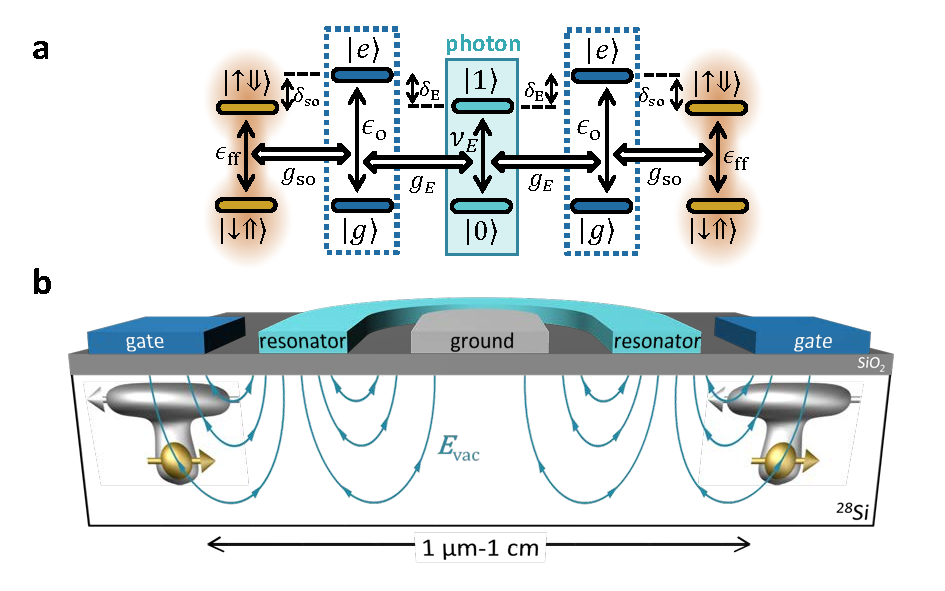
\includegraphics[width=\textwidth]{polished/cqed.pdf}
	\caption[Coupling to a resonator]{\textbf{Coupling to a resonator}.
		\textbf{a}, Level diagram for distant flip-flop qubit coupling via a microwave resonator showing photon number states and off-resonant charge states. 
		\textbf{b}, Device scheme for coupling qubits via a photonic link. Distant donors, placed next to the resonator center line and biased to their ionization point, are subject to the vacuum electric field $\textit{\textbf{E}}_{\rm vac}$ of a shared microwave resonator.}
	\label{fig:cqed}
\end{figure}

In order to reach the long-term goal of a large-scale quantum processor, wiring up the control and read-out lines for each individual qubit is not trivial, given the high density in typical spin qubit architectures \cite{Vandersypen2016}. Recent solutions include cross-wiring using multilayer lithography \cite{Hill2015} or floating gate electrodes inspired by dynamic random access memory systems \cite{Veldhorst2017}. In both cases, using flip-flop qubits with long-distance interactions would result in widely spaced donors and loose fabrication tolerances. In addition, since flip-flop qubits are coupled via electric fields, they could be spaced further apart by using electrical mediators. These include floating metal gates \cite{Trifunovic2013} or even microwave resonators. Indeed, the use of electric dipole transitions allows a natural integration of donor-based spin qubits into a circuit-Quantum Electrodynamics (QED) architecture \cite{Blais2004,Childress2004,Xiang2012,Mi2017} (see Fig. \ref{fig:cqed}b for a possible device layout).

A full quantum mechanical treatment yields a charge-photon coupling rate given by Eq. \ref{eq:g_E}, with $\nu_E$ now representing the resonator fundamental mode frequency and $E_{\rm ac}$ the resonator vacuum field, $E_{\rm vac}$ . Again, it is best to have the charge excited state detuned from the flip-flop transition and resonator photon (see Fig. \ref{fig:cqed}a), therefore minimizing charge excitation while retaining a second-order flip-flop-photon coupling given by Eq. \ref{eq:g_E_ff}. Assuming $\delta_{\rm so}\approx\delta_E\approx 10g_{\rm so}\approx 10g_E$, a $d=15$~nm deep $^{31}$P flip-flop qubit would be coupled to photons at a $g^{\rm ff}_E\approx3$~MHz rate. This is three orders of magnitude faster than the electron-spin coupling rate to a resonator via its magnetic vacuum field \cite{Tosi2017,Haikka2017}, and comparable to the coupling strength obtained by using strong magnetic field gradients \cite{Hu2012,Viennot2015}, but without the need to integrate magnetic materials within a superconducting circuit. This assumes a vacuum field amplitude $E_{\rm vac}\approx 30$~V/m, which can be obtained by using tapered coplanar waveguide or high-inductance resonators \cite{Samkharadze2016}.

The possibility of coupling the qubits to microwave photons provides a path for dispersive qubit readout, as well as for photonic interconnects. Near-quantum limited amplifiers have recently become available to obtain excellent readout speed and fidelities \cite{Castellanos2008}. The resonator can also be used as a quantum bus to couple two spin qubits separated by as far as 1~cm (Fig. \ref{fig:cqed}c), a distance given by the mode wavelength. Fig. \ref{fig:cqed}a shows the detailed energy level diagram. To avoid losses from photon decay, the qubits should be detuned from the resonator by an amount much greater than the qubit-photon coupling rates. Assuming $\delta^{\rm ff}_E=10g_{E}^{\rm ff}$, where $\delta^{\rm ff}_E=\nu_E-\epsilon_{\rm ff}$, the effective 2-qubit coupling $g_{\rm 2q}^{\rm ff}\approx(g_E^{\rm ff})^2/\delta^{\rm ff}_E\approx 0.3$~MHz yields a $\sqrt{i\mathrm{SWAP}}$ gate that takes only $0.4~\mu$s.

Thus, microwave resonators could be also used to interface donors with superconducting qubits \cite{Barends2014,Devoret2013}, for the long-term goal of a hybrid quantum processor that benefits from the many advantages of each individual architecture \cite{Xiang2012}.

\section{Conclusion}
In conclusion, we have presented a way to encode quantum information in the electron-nuclear spin states of $^{31}$P donors in silicon, and to realize fast, high-fidelity, electrically-driven universal quantum gates. 

\begin{figure}
	\centering
	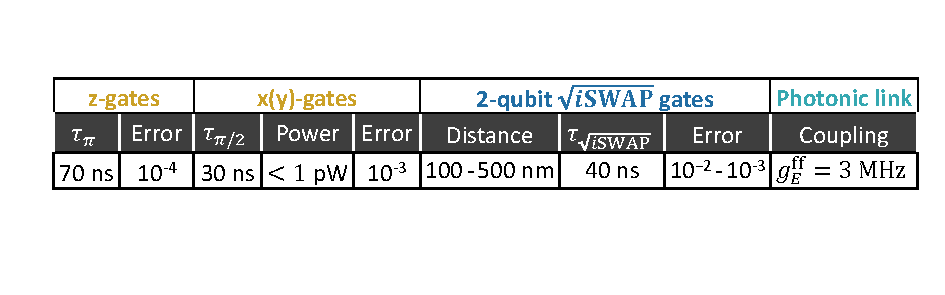
\includegraphics[width=\textwidth]{polished/merits.pdf}
	\caption[Gate performance summary]{\textbf{Gate performance summary}. Figures of merit summarizing the speed and error rates of different gate schemes present in this chapter, assuming realistic noise sources. }
	\label{fig:performance}
\end{figure}


Fig. \ref{fig:processor}a summarizes the key figures of merit of our flip-flop qubits coupled by electric dipole interactions. Fast 1-qubit $x$-gates are attainable with low electric drive power and error rates $\sim10^{-3}$. 2-qubit $\sqrt{i\mathrm{SWAP}}$ gates are fast and with error rates approaching $10^{-3}$. At the end of all operations, the phase of each qubit can be corrected, via adiabatic $z$-gates, in fast time scales and low error rates $\sim10^{-4}$. These values are based on current experimentally known values of charge noise in silicon devices \cite{Freeman2017}, and are possibly amenable to improvement through better control of the fabrication parameters. More advanced control pulse schemes could allow for faster gates with less leakage \cite{Motzoi2009,Ghosh2017,Werschnik2007}, and active noise cancellation techniques, $e.g.$ pulses for gate time jitter \cite{Hill2007} or decoherence \cite{VanDerSar2012} suppression, could further improve gate fidelities. 

Consequently, our proposal provides a credible pathway to the construction of a large-scale quantum processor as it not only features qubits with low error rates, compatible with fault-tolerant quantum error correction but also enables large qubit spacing, not requiring atomic-scale precision in the qubit placement.
 
% Chapter Template

\chapter{The nuclear spin qubit with an electric dipole transition} % Main chapter title

\label{Chapter3} 

\noindent\hrulefill
\vspace{0.5cm} %\hspace{2cm}
%\small
\begin{flushright}
        ``\emph{I’ve yet to see any problem, however complicated, which when you looked at it the right way didn’t become still more complicated.}"
\\ 
--Poul Anderson, \textit{Call Me Joe} \\
%“The most complicated skill is to be simple.” ―Dejan Stojanovic
\end{flushright}

\vspace{0.5cm}


\noindent\hrulefill
\vspace{0.5cm} %\hspace{2cm}
\\
%\small
\hangindent=4cm
%\noindent
\\
The nuclear spin state of a phosphorus donor in isotopically enriched silicon-28 is an excellent host to store quantum information in the solid state. The spin's insensitivity to electric fields yields a solid-state qubit with record coherence times but also renders coupling to other quantum systems very challenging. In this chapte, we describe how to generate a strong electric dipole ($>100$ D) at microwave frequencies for the nuclear spin. This is achieved by applying a magnetic drive to the electrically controlled flip-flop qubit. The dipole then allows for coupling to microwave resonators, with a vacuum Rabi splitting of the order of 1 MHz. This work brings the $^{31}$P nuclear qubit into the realm of hybrid quantum systems and opens up new avenues in quantum information processing.
\\ \\
\scriptsize
\hangindent=4cm
The work presented in this chapter has been published in:\\
G. Tosi, F. A. Mohiyaddin, \textbf{S. Tenberg}, A. Laucht, A. Morello. ``Robust electric dipole transition at microwave frequencies for nuclear spin qubits in silicon.'' \textit{Physical Review B} vol. 98, 075313 (2018).\\
\\
\footnotesize
\hangindent=4cm
\textbf{The author acknowledges G. Tosi for the conception of the idea and the bulk of the simulation work and F. A. Mohiyaddin for tight-binding simulations and electric modelling.}\\

%\vspace{0.5cm}

\noindent \hrulefill
\clearpage

\normalsize


\section{Introduction}

The nuclear spin of a phosphorus donor in silicon has long been the subject of much study in the context of solid-state quantum information processing, either as a qubit cell for large-scale quantum processors \cite{Kane1998,OGorman2016,Hill2015}, or a memory for long-lived quantum information storage \cite{Morton2008,Freer2017}. Whether in ensemble form \cite{Saeedi2013} or as individual qubit \cite{Muhonen2014}, the $^{31}$P nuclear spin has record-long coherence times, thanks to its insensitivity to electric fields and the possibility to drastically reduce magnetic environmental noise by hosting it in isotopically pure $^{28}$Si \cite{Itoh2014}. However, it cannot trivially be coupled to other quantum systems, and therefore all quantum computing proposals so far impose short interaction distances and slow quantum gate operations \cite{Kane1998,OGorman2016,Hill2015}.

In the hybrid approach to quantum information processing \cite{Xiang2012}, different quantum systems interact in a large architecture that benefits from the best properties of each system, which are often coupled together via microwave resonators. In order to couple to individual spin qubits, the resonator vacuum field can be enhanced by shrinking its dimensions in the vicinity of the spin qubit, thereby enhancing the spin-photon coupling rate \cite{Tosi2017,Jenkins2016,Haikka2017,Sarabi2018}. However, having a Zeeman splitting in the radio-frequency range and a null electric dipole, phosphorus nuclear-spins do not interact naturally with microwave resonators.

The artificial creation of electric dipole transitions has been proposed for different spin systems \cite{Pioro-Ladriere2008,Shi2012,Russ2017,Salfi2016,Tosi2017} as a way to facilitate scalability. The challenge here is how to make the spin drivable by electric fields without making it too susceptible to electrical noise, which can be significant in nanoscale electronic devices. In this chapter, we show how to engineer a strong electric dipole transition at microwave frequencies for the nuclear spin, based on the flip flop qubit and our finding from chapter \ref{Chapter2}, by applying an oscillating magnetic field to the nucleus while the electron is shared between the donor and a quantum dot defined at the Si/SiO$_2$ interface \cite{Calderon2009,Veldhorst2014, Tosi2017,Harvey-Collard2017}. While the admixture of spin and charge states can potentially make the system very sensitive to electric noise, we show that the nuclear spin precession frequency and electric dipole strength can be rendered highly immune to electrical noise by a peculiar choice of spin-charge hybridization, same than for the flip flop qubit. By providing a robust coupling between the nuclear spin and electric fields, our scheme opens up new avenues to couple $^{31}$P qubits to other quantum systems, including microwave resonators, superconducting qubits, or simply other nuclear spins but at distances and with speeds that had not been anticipated so far.


\section{Second-order Raman drive of a $^{31}$P nuclear spin} \label{sec:Raman}


\begin{figure}
\centering
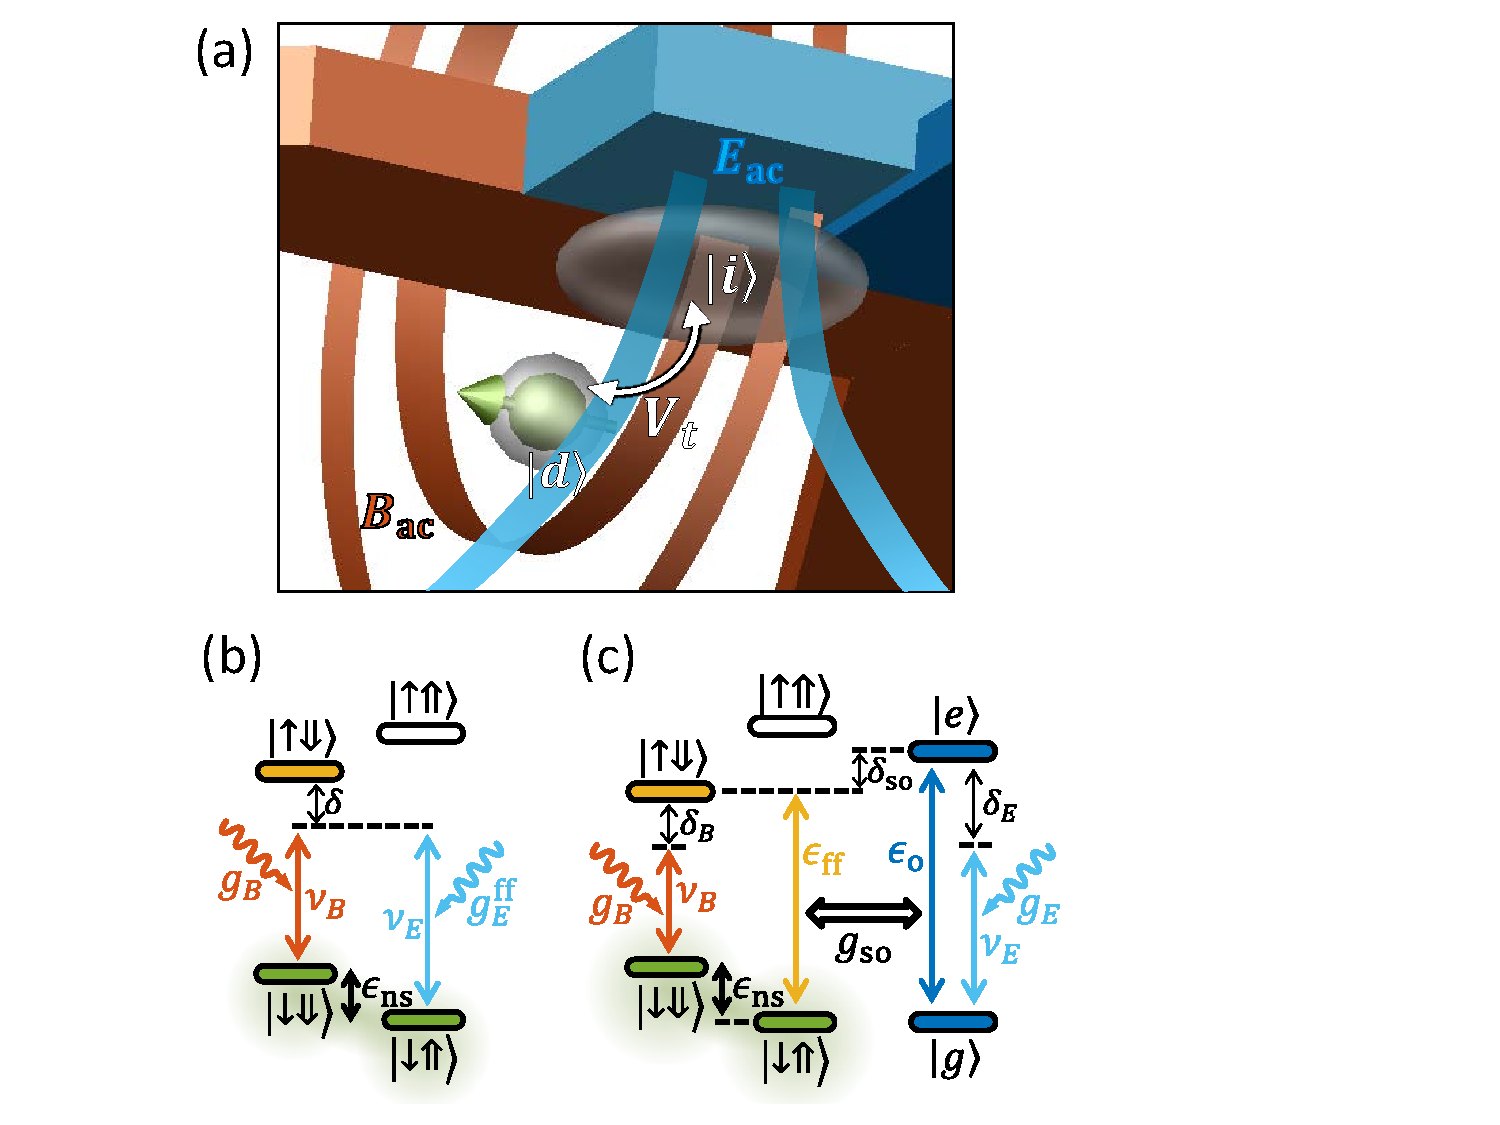
\includegraphics[width=0.8\columnwidth]{fig1_Raman_v5}
\caption[Nuclear Raman transition]{\textbf{Nuclear Raman transition. a}, Components of a Raman-enabled Si:P nuclear electric dipole transition. The electron  spatial wavefunction (transparent gray) is shared between an interface-dot, $|i\rangle$, and a donor-bound state, $|d\rangle$, which are coupled by a tunnel rate $V_t$. Metallic gates (blue) on top of SiO$_2$ dielectric (not shown) control the electron charge state via a static vertical field $E_{\rm dc}$, and can introduce an oscillating electric field $E_{\rm ac}$. In a circuit-Quantum Electrodynamics setup, the electrostatic gate can be replaced by the inner conductor of a microwave resonator, and $E_{\rm ac}$ by the vacuum field of such resonator. A nearby broadband antenna \cite{Dehollain2014} (brown) provides the magnetic drive $B_{\rm ac}$. 
\textbf{b} Simplified energy level diagram for Raman-drive of the Si:P nuclear-spin qubit, with energy splitting $\epsilon_{\rm ns}$. The second-order Raman drive is obtained by combining the microwave electric and magnetic drives, having frequencies $\nu_B$ and $\nu_E$, respectively, and coupling rates $g_B$ and $g_E^{\rm ff}$, respectively. The drive is detuned by a frequency $\delta$ from the $\ket{\uparrow \Downarrow}$ state. 
\textbf{c} Expanded energy diagram including the charge states $\ket{g}$ and $\ket{e}$.
}
\label{fig:Raman}
\end{figure}


The base of our proposal for an electrically accessible nuclear qubit is the flip flop qubit, as described in chapter \ref{Chapter2}, with the Hamiltonian $\mathcal{H}_{\rm ff}$ from eq. \eqref{eq:H_ff_ge}. 

The electron and nuclear spins can be coherently driven by conventional magnetic resonance transitions using oscillating magnetic fields at microwave \cite{Pla2012} and radio frequencies \cite{Pla2013} (see chapter \ref{sec:magRes}). In particular, the nuclear spin transition frequency when the electron spin is $\ket{\downarrow}$ (i.e. the $\ket{\downarrow \Uparrow} \leftrightarrow \ket{\downarrow \Downarrow}$ transition) is:
\begin{equation} \label{eq:epsilon_ns}
\epsilon_{\rm ns}(A) = \gamma_nB_0 + A/2.
\end{equation}


Now we show how the flip-flop transition provides a way of controlling the nuclear spin state without any radiofrequency field, by using instead two microwave-frequency excitations, one of which is electric, as illustrated in figure \ref{fig:Raman}a. This has important advantages over magnetic-only schemes \cite{Morton2008,Freer2017}, since it allows coupling a nucleus to the vacuum electric field of a microwave cavity, or to another nucleus similarly equipped with an electric dipole, as we will show below. The key idea is to combine the electrical drive of the flip-flop transition with an additional magnetic drive $B_{\rm ac}\cos(2\pi\nu_Bt)$, perpendicular to the static $B_0$ (Fig \ref{fig:Raman}a), where the Hamiltonian is 

\begin{equation}
\mathcal{H}_{\rm ESR}=B_{\rm ac}\cos(2\pi\nu_Bt)\left(\gamma_e S_x-\gamma_n I_x\right)
\end{equation}

which gives the full nuclear qubit Hamiltonian
\begin{equation}
\mathcal{H}_{\rm ns}=\mathcal{H}_{\rm ff}+\mathcal{H}_{\rm E}+\mathcal{H}_{\rm ESR}.
\end{equation}

 This magnetic drive is the conventional electron spin resonance (ESR) transition, that couples the electron spin states $\lvert\downarrow\Downarrow\rangle$ and $\lvert\uparrow\Downarrow\rangle$ at a rate:
\begin{equation}
g_{B}=\bra{\downarrow}\mathcal{H}_{\rm ESR}\ket{\uparrow}= \gamma_eB_{\rm ac}/4.
\end{equation}

Combining these two driving fields results in a process analogous to a Raman transition \cite{Kok2010}, as shown in Fig. \ref{fig:Raman}b: with the electron in the ground spin state $\ket{\downarrow}$, the AC electric and magnetic fields drive the nuclear-spin ``up'', $\lvert\downarrow\Uparrow\rangle$, and ``down'', $\lvert\downarrow\Downarrow\rangle$, states, respectively, to a virtual level detuned from the $\lvert\uparrow\Downarrow\rangle$ state by $\delta\gg g_B,g_E^{\rm ff}$. As a result, the nuclear spin is driven via a second order process, with minimal excitation of the electron spin, at a rate:

\begin{eqnarray}
\label{eq:g_E^ns_simple}
g_E^{\rm ns} & = & \frac{\left|\bra{\Downarrow \downarrow g} H_{ns} \ket{\Uparrow \downarrow g} \bra{\Downarrow \downarrow g} H_{ns} \ket{\Uparrow \downarrow g} \right|}{E_{\Downarrow \downarrow g}-E_{\Uparrow \downarrow g}}\\
& = & \frac{g_B g_E^{\rm ff}}{\delta}.
\end{eqnarray} 

This can be interpreted such that the microwave magnetic drive $B_{\rm ac}$ creates an electric dipole transition for the nuclear spin mediated by the flip-flop qubit, with strength:

\begin{equation}
p_E^{\rm ns} = \frac{4 g_E^{\rm ns}}{E_{\rm ac}} = \frac{4 g_B g_{E}^{\rm ff}}{E_{\rm ac} \delta}.
\label{eq:pns}
\end{equation}

The coupling $g_{E}^{\rm ff}$ between the flip-flop qubit and the AC electric field corresponds to a strong electric-dipole flip-flop transition ($\sim80$~Debye, assuming $\delta_{\rm so}=10g_{\rm so}$). Combining the strong flip-flop drive with the magnetic drive at rate $g_B$ (Eq.~\ref{eq:g_E^ns_simple}) results in a strong electric dipole transition for the nuclear spin ($\sim8$~Debye, assuming $\delta=10g_B$). Fig. \ref{fig:Raman}c shows the level diagram for the nuclear spin Raman transition taking the electron charge levels into account.

However, since the nuclear transition frequency depends linearly on $A$ (see Eq.~\ref{eq:epsilon_ns}), and $A$ is a very sensitive function of electric field near the donor ionization point, electrical noise in the device will cause fast dephasing of the nuclear precession.


\section{Robust electric dipole transition of a Si:P nuclear spin} \label{sec:robust}

\subsection{Electron, nuclear and charge hybridization} \label{sec:nuchybrid}

\begin{figure}
	\centering
	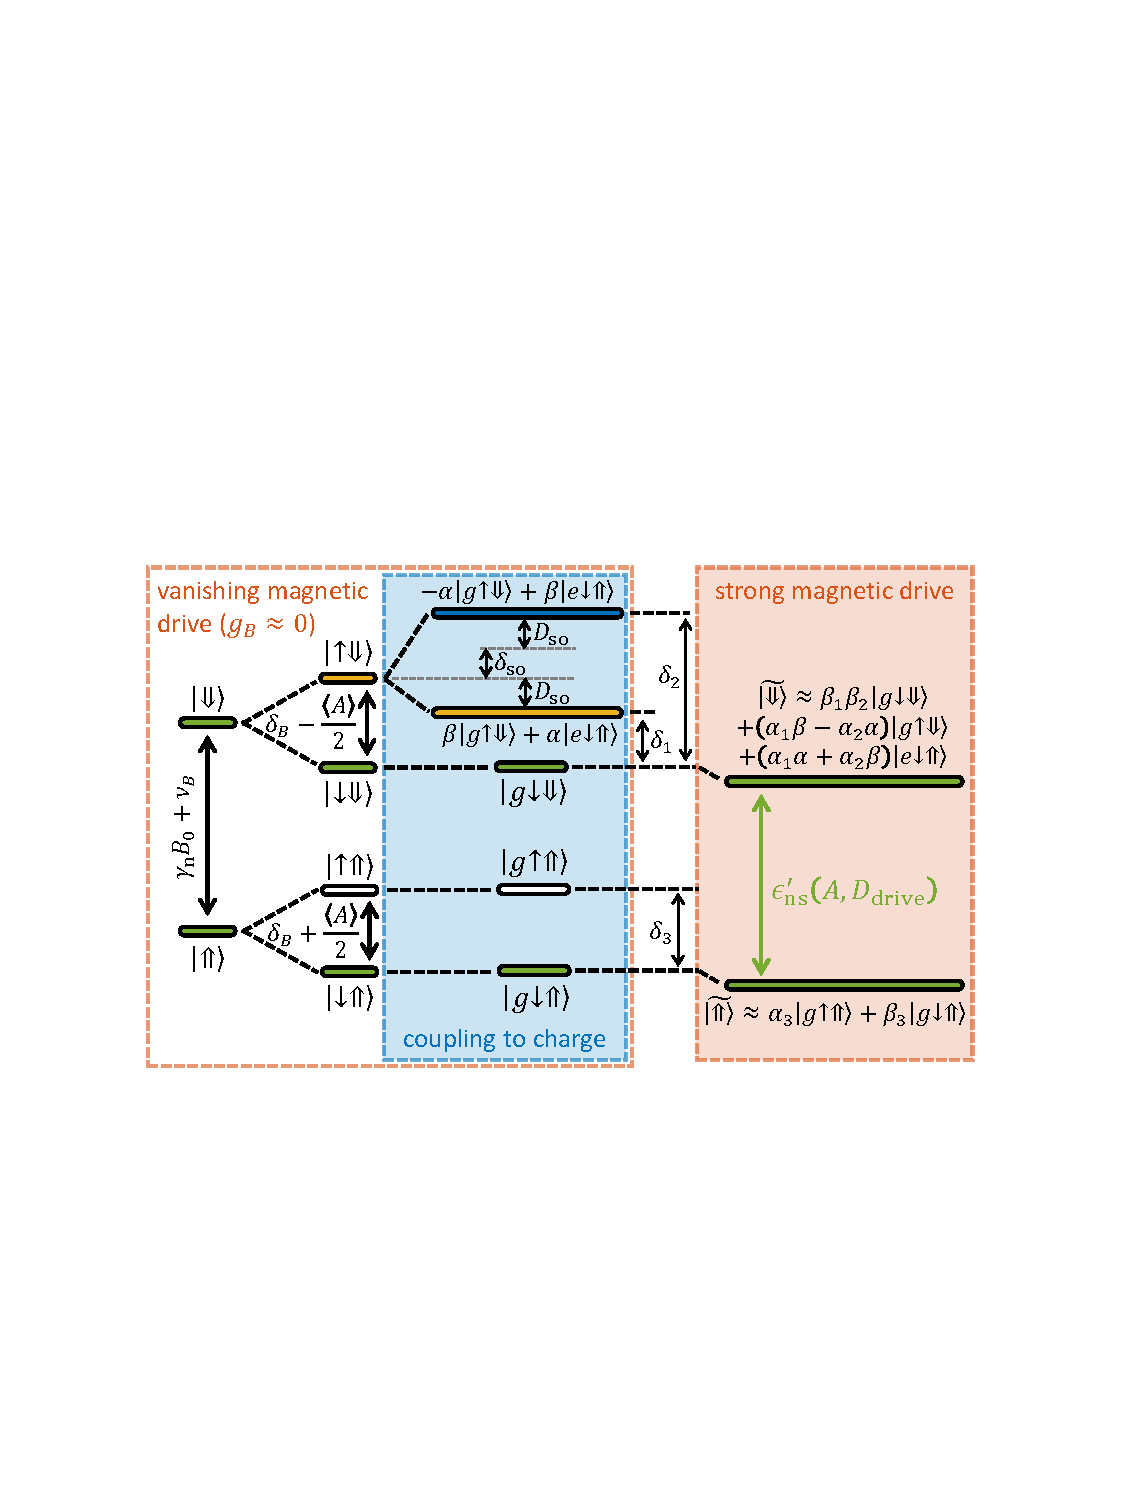
\includegraphics[width=\columnwidth]{fig2_levels}
	\caption[Nuclear spin level diagram with a strong magnetic drive]{\textbf{Nuclear spin level diagram with a strong magnetic drive}
 		Nuclear spin levels in the rotating frame of the magnetic drive $B_{\rm ac}$ at frequency $\nu_B$. From left to right, the system eigenstates are shown while adding the electron spin state, then the charge state, then increasing the strength of the magnetic drive. See main text for a detailed description.}
	\label{fig:levels}
\end{figure}

We now show that, by adopting a different choice of device tuning, the nuclear spin can be made largely insensitive to electrical noise, while having its electric dipole transition increased even further. This is achieved by tuning the charge qubit in resonance with the flip-flop qubit ($\epsilon_{\rm o} \approx \epsilon_{\rm ff}$, i.e. $\delta_{\rm so}\approx 0$), the magnetic drive in resonance with the electron spin ($\delta_B = \gamma_eB_0 - \langle A \rangle /2 -\nu_B\approx 0$), and the electric drive in resonance with the flip-flop (and charge) qubit ($\delta_E \approx 0$). In this strongly hybridized regime, second-order perturbation theory can not be directly applied. We therefore analyze the nuclear spin Hamiltonian $H_{\rm ns}$ by expressing it in the rotating frame of the magnetic drive by using the transformation:
\begin{subequations}
\begin{equation}
\mathcal{H}'=U^\dagger\mathcal{H}_{ns}U-i\hbar U\dot{U}^\dagger,
\end{equation}
\begin{equation}
U=e^{i2\pi\nu_Bt\left(S_z+I_z\right)}.
\end{equation}
\end{subequations}
We get

\begin{equation}
i\hbar U\dot{U}^\dagger=h\nu_B\left(S_z-I_z\right)
\end{equation}

and with $\cos(2\pi\nu_B t)=\frac{1}{2}\left(e^{i2\nu_B t}+e^{-i2\nu_B t}\right)$ follows

\begin{equation}
UH_{\rm ESR}U^\dagger=\frac{B_{\rm ac}}{2}\left[\gamma_e
\begin{pmatrix}
0 & e^{2\cdot i2\pi\nu_Bt}+1\\
e^{-2\cdot i2\pi\nu_Bt}+1 & 0
\end{pmatrix}-
\gamma_n\begin{pmatrix}
0 & e^{2\cdot i2\pi\nu_Bt}+1\\
e^{-2\cdot i2\pi\nu_Bt}+1 & 0
\end{pmatrix}\right]
\end{equation}

We neglect the counter-rotating terms, according to the rotating wave approximation and arrive at the transformed Hamiltonian of 

\begin{multline} \label{eq:H_nsRot}
\mathcal{H}'=\underbrace{\left(\gamma_e B_0 - \nu_B\right)}_{\delta_B}S_z-(\gamma_nB_0+\nu_B)I_z\\
+\frac{B_{ac}}{2}\left(\gamma_eS_x-\gamma_nI_x\right)+\mathcal{H}_{\rm orb}+\mathcal{H}_A^{\rm orb}+\mathcal{H}_E,
\end{multline}

where the magnetic drive is time-independent. 

The dominant energy scale in the above Hamiltonian is given by the term $-(\gamma_nB_0+\nu_B)I_z$, which represents the energy splitting of the nuclear spin states, but shifted to microwave frequencies by the transformation to the rotating frame of $\mathcal{H}_{\rm ESR}$. The corresponding energy levels are shown as $\ket{\Uparrow}, \ket{\Downarrow}$ at the left-most end of Fig.~\ref{fig:levels}. These levels are further split by the electron spin Hamiltonian, $\left(\delta_B+\langle A\rangle I_z\right)S_z+2g_BS_x$, where the expectation value of the hyperfine coupling $\langle A\rangle$ depends on the electron charge state, yielding the electron-nuclear spin levels shown in Fig. \ref{fig:levels}, depicted in the limit of vanishing $B_{\rm ac}$ (and therefore $g_B$) (see Fig. \ref{fig:hybridlevels}). In this case, the nuclear-spin transition frequency, in the rotating frame, with the electron in the ground state, is:

\begin{equation} \label{eq:e_ns}
\epsilon'_{\rm ns}(A) = \gamma_nB_0 + \nu_B + \langle A\rangle/2.
\end{equation}

\begin{figure}
\centering
	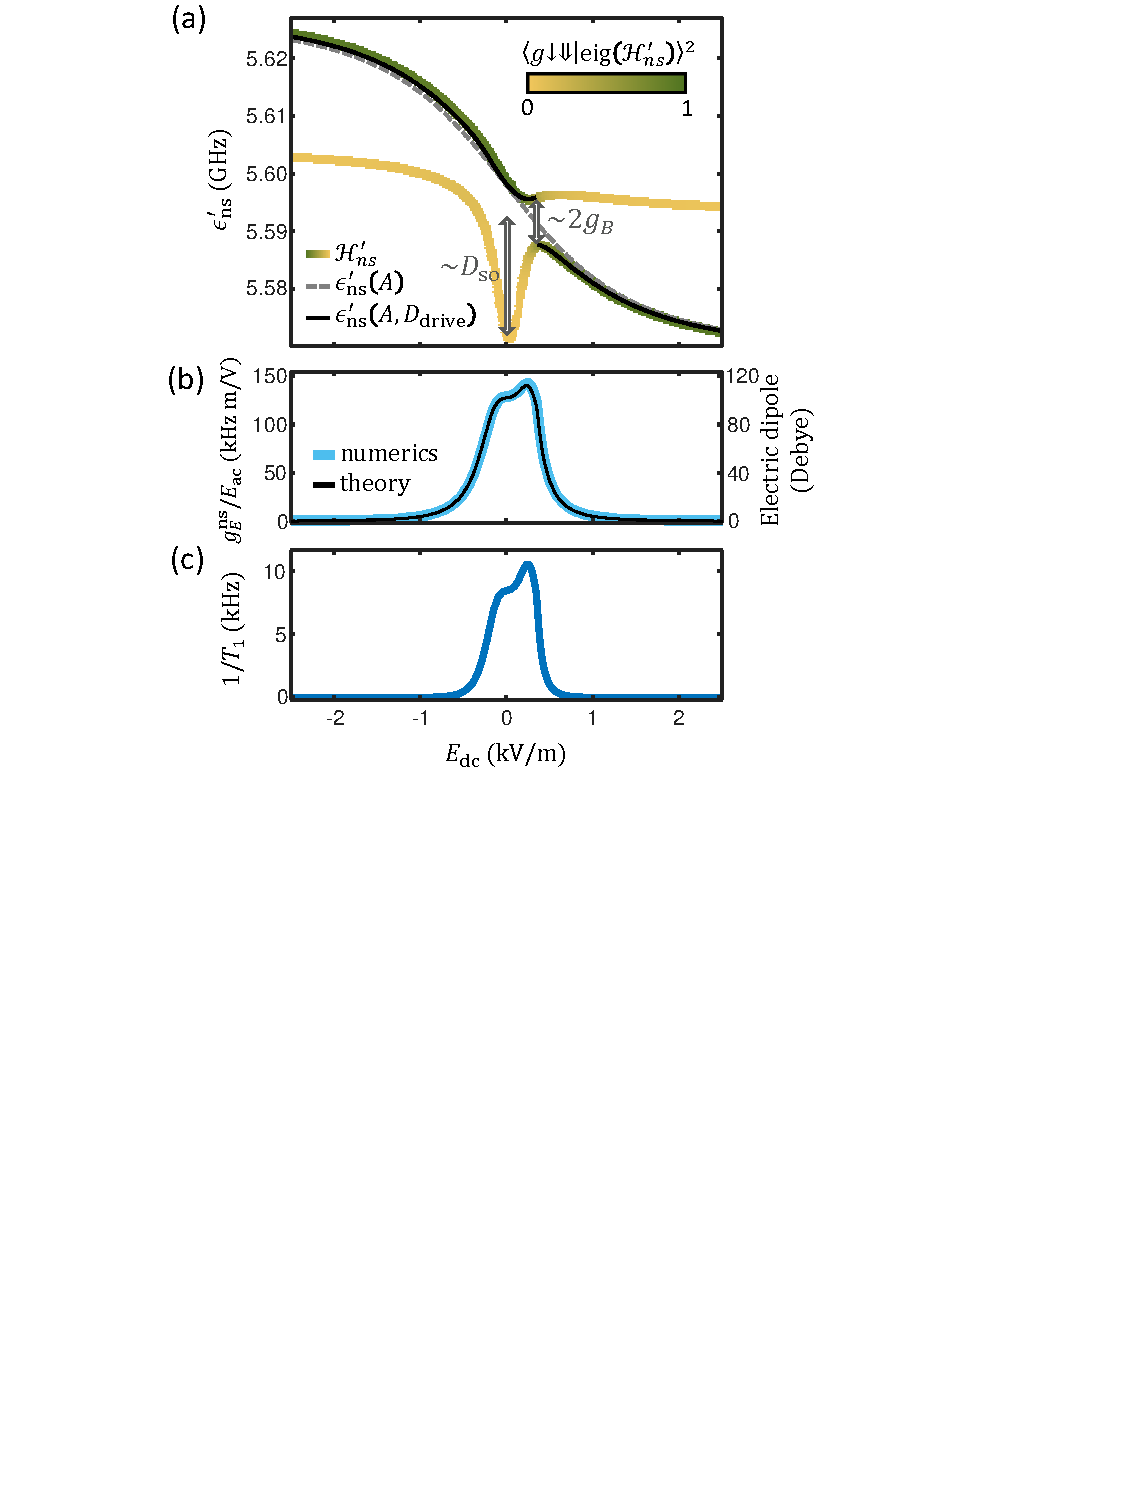
\includegraphics[width=0.9\columnwidth]{fig3_clock_v2}
	\caption[Nuclear qubit dispersion, dipole strength and relaxation]{
	\textbf{Nuclear qubit dispersion, dipole strength and relaxation. a}, Nuclear spin transition frequency $\epsilon'_{\rm ns}$ in the rotating frame of the magnetic drive $B_{\rm ac}$, as a function of the static vertical electric field $E_{\rm dc}$ across the donor-dot system, for vanishing magnetic drive ($\epsilon'_{\rm ns}(A)$ -- Eq.~\ref{eq:e_ns}, grey dashed line) and strong magnetic drive ($\epsilon'_{\rm ns}(A,D_{\rm drive})$ -- Eq.~\ref{eq:e_ns_Ddrive}, black solid line). We have assumed $B_0=0.2$~T, $B_{\rm ac}=0.6$~mT, $d=15$~nm and $V_t\approx \epsilon_{\rm ff}$ and $\nu_B\approx\gamma_eB_0-A/4$ (since $\langle A \rangle = A/2$ at the ionization point). Green/yellow lines show transition frequencies calculated numerically from the Hamiltonian in Eq. \ref{eq:H_nsRot}. The color indicates the degree of admixture of the bare $\ket{g\downarrow\Downarrow}$ state into the higher $\mathcal{H}'_{ns}$ eigenstate corresponding to each transition. The nuclear spin transition (predominantly $\ket{g\downarrow\Uparrow}\leftrightarrow\ket{g\downarrow\Downarrow}$, green) anticrosses a flip-flop transition (predominantly $\ket{g\downarrow\Uparrow}\leftrightarrow\ket{g\uparrow\Downarrow}$, yellow) at $E_{\rm dc}=350$~V/m, with a splitting $\sim2g_B$ set by the strength of the magnetic drive. The flip-flop transition is strongly shifted by $D_{\rm so}$, due to its coupling to the charge qubit states around $E_{\rm dc}=0$. At $E_{\rm dc}=250$~V/m, the nuclear-spin excited eigenstate has $\sim75\%$ of $\ket{g\downarrow\Downarrow}$ and is robust against electrical noise ($\partial\epsilon'_{\rm ns}/\partial E_{\rm dc}=0$).
	\textbf{b} Nuclear electric dipole strength $p_E^{\rm ns}=\partial g_E^{\rm ns} / \partial E_{\rm ac}$ obtained from Eqs.~\ref{eq:g_E^ns} (theory, black line), or for numerical diagonalization of the full Hamiltonian $\mathcal{H}'$ under $E_{\rm ac}$ drive (numerics, light blue line). For the choice of parameters used in this figure,  $p_E^{\rm ns}$ peaks where $E_{\rm dc}=250$~V/m. 
		\textbf{c} Nuclear spin relaxation rate $1/T_{\rm 1,ns}$ in the presence of the magnetic drive $B_{\rm ac}$ and the effect of coupling to phonons via charge states, Eq.~\ref{eq:T1ff}.
	}
	\label{fig:clock}
\end{figure}

In Fig. \ref{fig:clock}a we plot $\epsilon'_{\rm ns}(A)$ (dashed line) by including the dependence of $\langle A \rangle$ on vertical electric field $E_{\rm dc}$ (from Eqs.~\eqref{eq:H_orb},\eqref{eq:H_A}). This is valid when the electron charge states are far detuned from the spin levels ($\delta_{\rm so}\gg g_{\rm so}$). The plot highlights the strong dependence of $\epsilon'_{\rm ns}$ on electric fields under such conditions. 

However, the nuclear spin dispersion changes dramatically when $\delta_{\rm so}$ approaches zero. In that case, $\mathcal{H}_A^{\rm orb}$ hybridizes the flip-flop and charge states, as shown in the blue panel within Fig. \ref{fig:levels}. The overall ground state is $\ket{g\downarrow\Uparrow}$, but the excited flip-flop state splits into two hybridized states $\beta \ket{g\uparrow\Downarrow}+ \alpha\ket{e\downarrow\Uparrow}$ and $-\alpha \ket{g\uparrow\Downarrow} + \beta\ket{e\downarrow\Uparrow}$, with:

\begin{subequations} \label{eq:alphabeta}
\begin{eqnarray}
\alpha=\frac{\theta}{\sqrt{\theta^2+1}},~~~\theta=\frac{\delta_{\rm so}-\sqrt{{\delta_{\rm so}}^2+4{g_{\rm so}}^2}}{2g_{\rm so}},
\end{eqnarray}
\begin{eqnarray}
\beta=\frac{\phi}{\sqrt{\phi^2+1}},~~~\phi=\frac{\delta_{\rm so}+\sqrt{{\delta_{\rm so}}^2+4{g_{\rm so}}^2}}{2g_{\rm so}},
\end{eqnarray}
\end{subequations}
so that $\alpha=\beta=1/\sqrt{2}$ for $\delta_{\rm so}=0$ (as Eq. \eqref{eq:ff_hybrid}). 

As a final step, by increasing the magnetic drive amplitude $B_{\rm ac}$, the Hamiltonian term $2g_BS_x$ couples the electron spin $\ket{\uparrow}$ and $\ket{\downarrow}$ states, further hybridizing the system eigenstates $\ket{g\downarrow\Downarrow}$ with the hybridized flip-flop states as well as $\ket{g\uparrow\Uparrow}$. Two of those eigenstates, which we call $\widetilde{\ket{\Downarrow}}$ and $\widetilde{\ket{\Uparrow}}$ (Fig.~\ref{fig:levels}, orange box), are chiefly composed of the tensor product of the nuclear $\ket{\Downarrow}$, $\ket{\Uparrow}$ states with the ground charge state $\ket{g}$ and the ground $\ket{\downarrow}$ electron spin state. They are obtained as:

\begin{eqnarray} \label{eq:tildestates}
\widetilde{\ket{\Downarrow}} & \approx & \beta_1 \beta_2\ket{g\downarrow\Downarrow} + \left(\alpha_1 \beta - \alpha_2 \alpha\right) \ket{g\uparrow\Downarrow} + (\alpha_1 \alpha + \alpha_2 \beta)\ket{e\downarrow\Uparrow}\\
\widetilde{\ket{\Uparrow}}&\approx & \alpha_3 \ket{g\uparrow\Uparrow} + \beta_3\ket{g\downarrow\Uparrow},
\end{eqnarray}
with coefficients $\alpha_i, \beta_i$ ($i=1,2,3$) given by:

\begin{subequations} \label{eq:alphaibetai}
\begin{equation} \label{eq:alpha1}
\alpha_1=\frac{\theta_1}{\sqrt{{\theta_1}^2+1}},~~~
\theta_1=\frac{\delta_1-\sqrt{{\delta_1}^2+(2{\beta g_B})^2}}{2\beta g_B}
\end{equation}
\begin{equation} \label{eq:beta1}
\beta_1=\frac{\phi_1}{\sqrt{{\phi_1}^2+1}},~~~
\phi_1=\frac{\delta_1+\sqrt{{\delta_1}^2+(2{\beta g_B})^2}}{2\beta g_B}
\end{equation}
\begin{equation} \label{eq:alpha2}
\alpha_2=\frac{\theta_2}{\sqrt{{\theta_2}^2+1}},~~~
\theta_2=\frac{\delta_2-\sqrt{{\delta_2}^2+(2\alpha g_B)^2}}{2\alpha g_B}
\end{equation}
\begin{equation} \label{eq:beta2}
\beta_2=\frac{\phi_2}{\sqrt{{\phi_2}^2+1}},~~~
\phi_2=\frac{\delta_2+\sqrt{{\delta_2}^2+(2{\alpha g_B})^2}}{2\alpha g_B}
\end{equation}
\begin{equation} \label{eq:alpha3}
\alpha_3=\frac{\theta_3}{\sqrt{{\theta_3}^2+1}},~~~
\theta_3=\frac{\delta_3-\sqrt{{\delta_3}^2+4{g_B}^2}}{2g_B}
\end{equation}
\begin{equation} \label{eq:beta3}
\beta_3=\frac{\phi_3}{\sqrt{{\phi_3}^2+1}},~~~
\phi_3=\frac{\delta_3+\sqrt{{\delta_3}^2+4{g_B}^2}}{2g_B}
\end{equation}
\end{subequations}

The energy splitting between $\widetilde{\ket{\Downarrow}}$ and $\widetilde{\ket{\Uparrow}}$, $\epsilon'_{\rm ns}$, equals the bare nuclear-spin transition, $\epsilon'_{\rm ns}(A)$ (Eq.~\eqref{eq:e_ns}), plus an amount that dependents on $E_{\rm dc}$:

\begin{equation} \label{eq:e_ns_Ddrive}
\epsilon'_{\rm ns}(A,D_{\rm drive})=\epsilon'_{\rm ns}(A)-D_{\rm drive}(E_{\rm dc}),
\end{equation}
where $D_{\rm drive}$ is an AC-Stark shift given by second order perturbation theory to (analogous to Eqs. \eqref{eq:Dorb}, \eqref{eq:Ddd}):
\begin{subequations}
\begin{equation} \label{eq:Ddrive}
D_{\rm drive}(E_{\rm dc})=\sum_{i=1,2,3}\frac{\delta_i}{2}\left(\sqrt{1+\left(\frac{2g_i}{\delta_i}\right)^2}-1\right),
\end{equation}
\begin{equation} \label{eq:g_alpha_beta}
g_1=\beta g_B,~~~~g_2=-\alpha g_B,~~~~g_3=g_B.
\end{equation}
\end{subequations}

This equation agrees with numerical simulations of the full Hamiltonian in the rotating frame of Eq.~\eqref{eq:H_nsRot} (Fig. \ref{fig:clock}a). Around the ionization point, the flip-flop transition (itself strongly affected by the hybridization with the charge state) anticrosses the nuclear spin transition (in the rotating frame), creating a region where $\partial\epsilon'_{\rm ns}/\partial E_{\rm dc}=0$, i.e. a first-order `clock transition' \cite{Bollinger1985,Wolfowicz2013} where $\epsilon'_{\rm ns}$ is insensitive to electric noise to first order. Further adjustment of the parameters allows for $\partial^2\epsilon'_{\rm ns}/\partial {E_{\rm dc}}^2=0$ (second-order clock transition), improving noise insensitivity even further.

In a key result of our proposal, the small admixture of the excited charge state, $\ket{e}$, into $\widetilde{\ket{\Downarrow}}$ creates an electric-dipole transition for the nuclear spin. Indeed, the $\widetilde{\ket{\Downarrow}} \leftrightarrow \widetilde{\ket{\Uparrow}}$ transition can be electrically-driven at a rate given by the charge admixture coefficients in Eq.~\ref{eq:alphaibetai} (see also Fig.~\ref{fig:clock}b):

\begin{equation} \label{eq:g_E^ns}
g_{E}^{\rm ns}=g_E\beta_3\left(\alpha_1\alpha+\alpha_2\beta\right),
\end{equation}

This electric dipole transition, at microwave frequencies, can reach $>100$~Debye around $E_{\rm dc}=0$ (Fig.~\ref{fig:clock}b). This means that even an extremely weak AC electric field, $E_{\rm ac}\approx 3$~V/m, can drive a nuclear spin transition at a MHz Rabi frequency. This is two orders of magnitude faster than the typical Rabi frequencies obtained with standard (NMR) magnetic drive at radiofrequency \cite{Pla2013}, and an order of magnitude faster than obtained (at very high electric drive amplitudes) in a recent experiment where electrically-driven NMR was achieved by modulating the quantization axis of the electron spin \cite{Sigillito2017}.

\subsection{Resilience against charge noise}

The issue of charge noise is of paramount importance in semiconductor spin qubits. It is known, experimentally and theoretically, that charge fluctuators yield a $1/\nu$ frequency dependence of the noise spectral density \cite{Paladino2014}. These models capture the averaged collective effect of many charge fluctuators on the qubit operation. In this case, charge noise results in a slow drift of the qubit electrostatic environment. Indeed, since individual qubit operations take less than a microsecond, the qubit environment is usually static within a single operations, but fluctuates in between operations. The estimating the noise in our system based on experimental results yields is 1.7~${\mu \rm eV}$ r.m.s. noise amplitude, which, given the distance between donor and interface $d \approx 15$~nm, corresponds to an r.m.s. noise on the amplitude of the vertical electric field of order 100~V/m (see chapter \ref{sec:noise}). Inserting this into our model of the qubit energy according to Eq. \eqref{eq:dephasing_rate} yields a predicted nuclear spin dephasing rate of order $1-10$~kHz. Note that, similarly to dressed states \cite{London2013,Laucht2016,Laucht2016a}, the addition of the strong magnetic drive has the effect of extending the coherence of our qubit. However, here the suppressed noise is of electrical nature (despite the drive being magnetic), given the particular hybridization with charge states.

We thus derived the striking result that the nuclear spin has a strong electric dipole despite being robust against electrical noise. This is because, while the qubit precession frequency is insensitive to noise, its effective transverse matrix element is strongly dependent on electric fields. Importantly, the electric dipole is induced on the nuclear spin  only around the flip-flop transition frequency, which is at several GHz. Since the charge and gate noise in nanoscale devices mainly has a $1/\nu$ spectrum, the power spectral density of the noise at the frequency that would affect the nuclear qubit is expected to be very weak. Moreover, at the same bias point where the CT ($\partial\epsilon'_{\rm ns}/\partial E_{\rm dc}=0$) for the nuclear energy takes place, the nuclear electric dipole itself is also first-order insensitive to electrical noise, since $\partial g_{E}^{\rm ns}/\partial E_{\rm dc}=0$ (Fig. \ref{fig:clock}b). A realistic $1.5~\mu$eV charge detuning noise \cite{Freeman2017} would make $g_{E}^{\rm ns}$ fluctuate by only $\sim2\%$. In other words, in this system both the free precession frequency and the Rabi frequency can be made first-order insensitive to charge noise.

As a final note, although we assumed $\delta_{\rm so} \rightarrow 0$, the electric and magnetic driving fields are still off-resonance with the eigenstates of the full Hamiltonian $\mathcal{H}_{\rm ns}$ due to the hybridized charge-flip-flop states, ensuring minimal excitation of the $\ket{\uparrow}$ and $\ket{e}$ states.

\subsection{Coupling to microwave cavity photons}

This strong electric dipole at microwave frequencies provides a pathway for strongly coupling $^{31}$P nuclear spins to microwave resonators \cite{Blais2004}, where a vacuum field $E_{\rm vac}$ of a few V/m can result in vacuum Rabi splittings around 1~MHz. This could be achieved \textit{e.g.} by connecting the top blue gate on Fig.~\ref{fig:Raman}a to the center pin of a superconducting coplanar waveguide resonator. Our proposal thus provides a solution to the fact that the standard (NMR) nuclear-spin transition does not naturally couple to microwave resonators. Similarly to other proposals  \cite{Pachos2002,Childress2004,Feng2008,Abanto2010}, here it is a classical drive ($B_{\rm ac}$) that enables coupling to a quantum field ($E_{\rm vac}$).

\subsection{Nuclear spin relaxation}

The engineered nuclear electric dipole also opens up a new pathway for nuclear spin relaxation: $\widetilde{\ket{\Downarrow}}$ can decay into $\widetilde{\ket{\Uparrow}}$ through a peculiar effect, where a photon from the driving field is combined with the nuclear spin energy (which is at radiofrequency) to emit a phonon at microwave frequency. The rate for this process can be roughly estimated as the admixture of the $\ket{e}$ charge excited state into the $\widetilde{\ket{\Downarrow}}$ eigenstate times the charge relaxation rate ${1}/{T_{1,\rm o}}$:

\begin{equation}\label{eq:T1ff}
\frac{1}{T_{1,\rm ns}}=\frac{|\widetilde{\bra{\Downarrow}}e\rangle|^2}{T_{1,\rm c}}\approx \frac{|\alpha_1\alpha+\alpha_2\beta|^2}{{T_{1,\rm c}}},
\end{equation}

where ${1}/{T_{1,\rm c}}=\Theta\epsilon_{\rm o}{V_t}^2$ (Ref.~\cite{Boross2016}), with $\Theta\approx2.37\times10^{-24}~{\rm s}^2$ determined by the silicon crystal properties. 

As Fig.~\ref{fig:clock}c shows, ${1}/{T_{1,\rm ns}}$ peaks, around the ionization point, at a value that is still two orders of magnitude slower than e.g. the spin's coupling rate to a microwave resonator, therefore allowing the strong coupling regime to be well within reach.


\subsection{Dependence of electric dipole strength and spin relaxation rate on frequency and field detuning} \label{supp:detdep}

In Fig.~\ref{fig:clock} we have shown an operation point ($E_{\rm dc}=250$~V/m and $\nu_B=5.565$~GHz) where the proposed nuclear spin electric dipole transition is robust against noise, i.e. both its precession frequency, $\epsilon_{\rm ns}'$, and electric dipole strength, $p^E_{\rm ns}=g_E^{\rm ns}/E_{\rm ac}$, are to first order insensitive to small perturbations of the static electric field. To understand how the system behaves when slightly detuned from the optimal working point, we calculate the dependence of the nuclear spin electric dipole strength $p^E_{\rm ns}$ and relaxation rate $1/T_{1, \rm ns}$ on the magnetic drive frequency, $\nu_B$, and on the static electric field, $E_{\rm dc}$. 

\begin{figure}
	\centering
	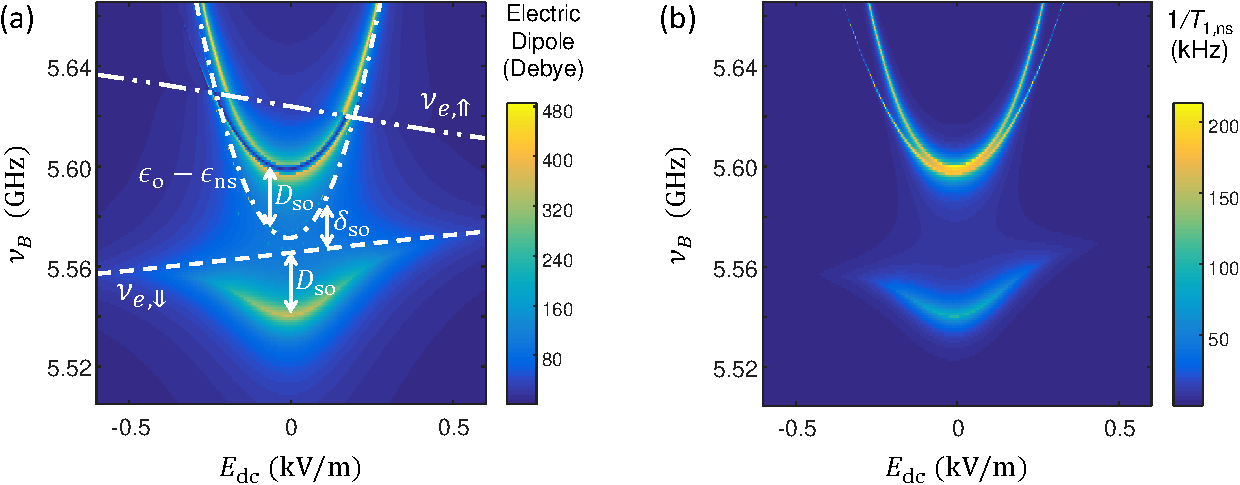
\includegraphics[width=1\textwidth]{fig4_v2}
	\caption[Nuclear electric dipole strength and relaxation as a function of electric field]{\textbf{Nuclear electric dipole strength and relaxation as a function of electric field. a},
	 Nuclear electric dipole strength $p_E^{\rm ns}$ and
		\textbf{b} nuclear spin relaxation rate $1/T_{\rm 1,ns}$, as a function of the donor-dot electric field detuning, $E_{\rm dc}$, and the magnetic drive frequency, $\nu_B$. $E_{\rm dc}=0$ is the ionization point. In \textbf{a}, the dashed line shows the ESR frequency $\nu_{e,\Downarrow}$ when the nuclear spin is in the  $\ket{\Downarrow}$ state, the dot-dashed line shows the charge qubit frequency minus the nuclear spin frequency, $\epsilon_{\rm o} - \epsilon_{\rm ns}$, and the dot-dot-dashed line the electron spin resonance frequency $\nu_{e,\Uparrow}$ when the nuclear spin is in the $\ket{\Uparrow}$ state. The charge and flip-flop states are detuned by $\delta_{\rm so}$, which is close to zero at $E_{\rm dc}=0$. Charge and flip-flop states then hybridize, shifting the system eigenenergies by an AC-Stark shift $D_{\rm so}$. The plots in Figs.~\ref{fig:clock}b,c correspond to specific line cuts of the graphs shown here, for $\nu_B=\nu_{e,\Downarrow}$ at $E_{\rm dc}=0$, \textit{i.e.} $\nu_B=5.565$~GHz.
	}
	\label{fig:fig4}
\end{figure}

The results are plotted in Fig. \ref{fig:fig4}. Both plots show two branches (bright yellow) where both dipole moment and relaxation rate are enhanced. To understand these branches, we refer to the level diagrams in Figs. \ref{fig:Raman}b,c. First, note that $\nu_B$ unequivocally sets the electric dipole transition frequency $\nu_E$ (in the simplest case, $\nu_E=\nu_B+\epsilon_{\rm ns}$). The two bright branches in  Fig.~\ref{fig:fig4}a,b correspond to $\nu_E$ being in resonance with either of the two charge-flip-flop hybridized states (yellow and blue states inside the light blue rectangle in Fig. \ref{fig:levels}). If the charge and flip-flop states were uncoupled or off-resonance, then the lower branch would simply correspond to the flip-flop dipole transition, $\nu_E=\nu_{e,\Downarrow}+\epsilon_{\rm ns}$ (where $\nu_{e,\Downarrow}$ is the electron spin resonance frequency when the nuclear spin is in the `down' state), which means that the magnetic drive frequency simply coincides with the electron spin resonance $\nu_B=\nu_{e,\Downarrow}$. This would represent a simple, on-resonance Raman transition, i.e. as in the sketch in Fig.~\ref{fig:Raman}b but where $\delta=0$. Then, the upper branches in Fig.~\ref{fig:fig4} would correspond to the pure charge transition, $\nu_E=\epsilon_{\rm o}$, or equivalently $\nu_B=\epsilon_{\rm o}-\epsilon_{\rm ns}$. However, since the charge and flip-flop states are coupled, they hybridize and further split the two branches by an amount equal to $D_{\rm so}$.

Upon closer inspection, the upper branch shows an extra subtle feature. This branch corresponds to excitation conditions that put the magnetic drive frequency close to the electron spin resonance frequency when the nuclear spin is in the $\ket{\Uparrow}$ state, $\nu_{e,\Uparrow}$. This, in turn, creates a pair of dressed electron spin states that further split the upper branch into two, separated by the ESR (magnetic) Rabi frequency of the $\nu_{e,\Uparrow}$ resonance. 

\section{Long-distance coupling of nuclear spin qubits} \label{sec:long}

\begin{figure}
\centering
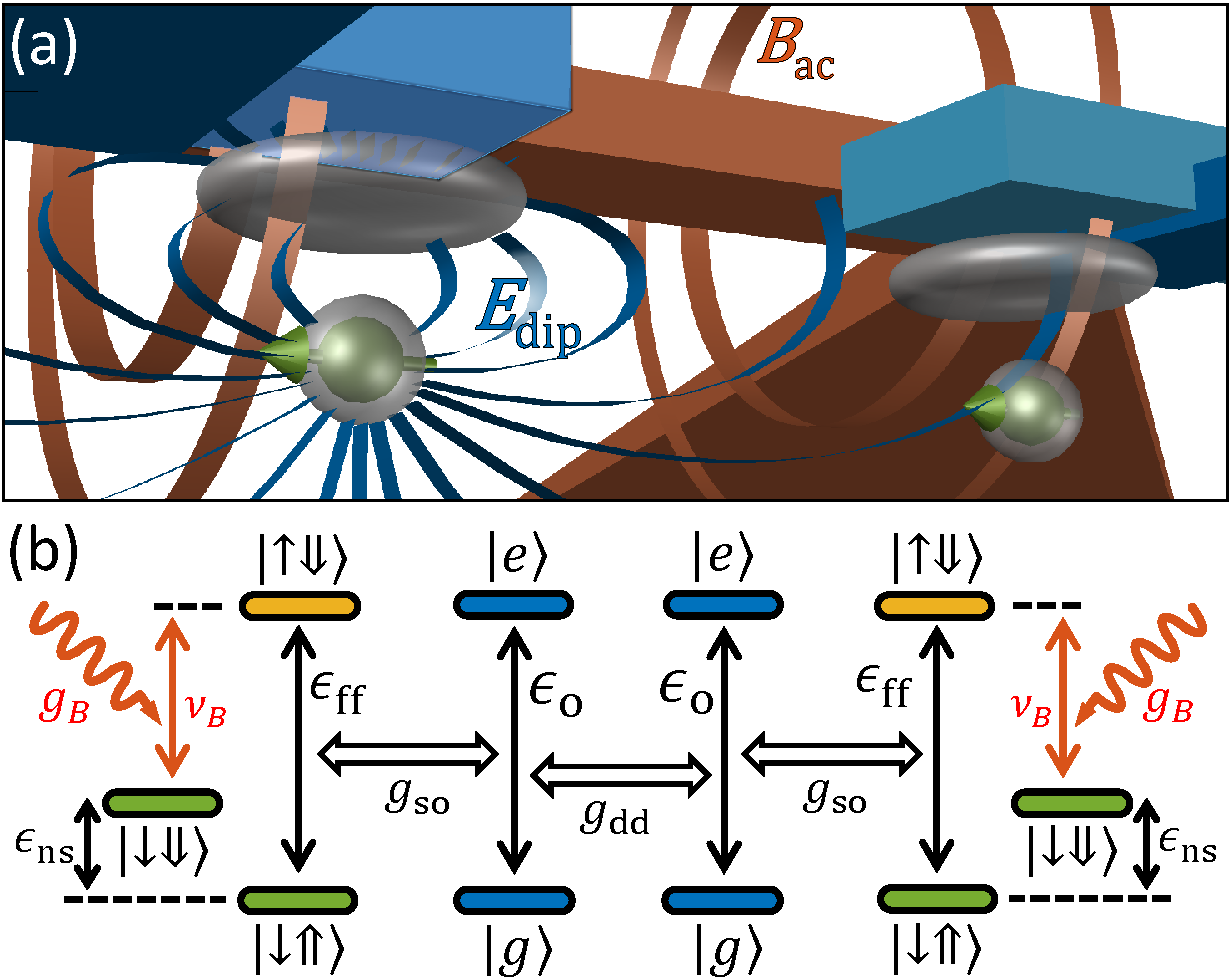
\includegraphics[width=0.9\columnwidth]{fig5_2-qubit_nuc}
\caption[Long distance coupling of two nuclear qubits]{
\textbf{Long distance coupling of two nuclear qubits. a}, Components and \textbf{b} level diagram for long-distance coupling of two $^{31}$P nuclear spins via electric dipole-dipole interactions. Each displaced electron produces an electric dipole field $E_{\rm dip}$ (shown only for one electron). The charge dipoles induced by displacing the electron wavefunction partly towards the interface dot interact with a strength $g_{\rm dd}$ (Eq.~\ref{eq:g_dd}), and the charge qubits interact with the flip-flop states with strength $g_{\rm so}$ (Eq.~\ref{eq:g_so}). Adding the (global) magnetic drive of strength $g_B$ and tuning the system to the fully-hybridized regime described in Sec.~\ref{sec:robust} results in a nuclear-nuclear coupling strength $g_{\rm 2q}^{\rm ns} \approx 0.55$~MHz at a $400$~nm distance (Eq.~\ref{eq:nucSWAP}).
}
\label{fig:2-qubit_nuc}
\end{figure}

We have shown in the previous section that a robust electric dipole at microwave frequencies is induced on the nuclear spin by the magnetic drive $B_{\rm ac}$, combined with the spin-charge hybridization that is obtained by displacing the electron from the donor towards an interface quantum dot. A natural and important extension of this effect is to exploit the induced electric dipole to achieve a long-distance coupling of the nuclear spins, mediated by long-range electric dipole interaction, similar as for the flip flop qubit in chapter \ref{Chapter2}, as illustrated in Fig. \ref{fig:2-qubit_nuc}a \cite{Tosi2017}. This dipole interaction between the charge qubits results in a coupling of $g_dd$ (eq. \eqref{eq:g_dd}). 

Two distant nuclear spin qubits can then be coupled when both electrons are around their ionization point, and an AC magnetic drive $B_{\rm ac}$ is applied (Fig. \ref{fig:2-qubit_nuc}a,b) to each of them, resulting in the electric dipole $p_E^{\rm ns}$ at microwave frequencies. For the operation parameters used in Fig.~\ref{fig:clock}, $\epsilon_{\rm o}\approx\epsilon_{\rm ff}\approx\nu_B+\epsilon_{\rm ns}$ and $g_B\ll g_{\rm so}$, the two-qubit coupling rate is obtained, via second-order perturbation theory, as:

\begin{eqnarray} \label{eq:nucSWAP}
g_{\rm 2q}^{\rm ns} & = & \bra{\tilde{\Downarrow}_1 \tilde{\Uparrow}_2}\mathcal{H}_{\rm ns}\ket{\tilde{\Uparrow}_1 \tilde{\Downarrow}_2}\\
 & =& \left(\frac{g_B}{g_{\rm so}}\right)^2g_{\rm dd},
\end{eqnarray}
 
which is valid if $g_B\ll (g_{\rm so})^2/g_{\rm dd}$. For two nuclear spins $r=400$~nm apart, $g_{\rm 2q}^{\rm ns}=0.55$~MHz, yielding a $\sqrt{i\mathrm{SWAP}}$ gate time of $\sim230$~ns. To put this in perspective, the Kane's proposal \cite{Kane1998} described a system of  two $^{31}$P nuclear spins placed $r=15$~nm apart, where a $\sqrt{i\mathrm{SWAP}}$ gate mediated by the electron spin exchange interaction requires $3~\mu$s -- an order magnitude slower, for over an order of magnitude tighter spacing. A recent proposal by Hill et al. \cite{Hill2015} describes a CNOT gate between nuclear spins mediated by the electron magnetic dipole interaction, wherein the 2-qubit gate time requires 300~$\mu$s for donors spaced $30$~nm apart -- three orders of magnitude slower than the electric-dipole mediated gate we have introduced here.


This method of coupling nuclear spin qubits at long distances via their induced electric dipole can be switched off completely -- $p_E^{\rm ns} \approx 0$ when the electron charge is moved back to the donor -- thus offering great flexibility in how multi-qubit operations are undertaken in a large array of qubits. The magnetic drive $B_{\rm ac}$ necessary to induce the dipole can be a global, always-on field, acting on every donor in the array. This can be optimally achieved by placing the device in a three-dimensional microwave cavity with good $B_{\rm ac}$ homogeneity \cite{Angerer2016}. Alternatively, $B_{\rm ac}$ could be delivered locally using a grid of microwave striplines \cite{Li2018}. The ``robust'' mode of operation described in Sec.~\ref{sec:robust} requires $\delta_B \approx 0$, i.e. $B_{\rm ac}$ in resonance with the electron spin transition. However, this resonance condition must be met while the donor is at the ionization point, where the hyperfine coupling is approximately half the value it has while the electron is fully at the donor ($\langle A\rangle \approx A/2$), thus $\nu_B \approx \gamma_e B_0 - A/4$. Therefore, idle qubits with the electron resting at the donor will be left unaffected by the global magnetic drive, and completely decoupled from both electric and magnetic AC-fields.


\section{Conclusion} \label{sec:conclusion}

The exceptional quantum coherence of $^{31}$P nuclear spins in isotopically enriched $^{28}$Si is experimentally well established \cite{Saeedi2013,Muhonen2014}. However, it has been widely accepted that using the $^{31}$P nuclear spin as the physical qubit in a quantum computer architecture requires dealing with the very small nuclear magnetic dipole, which renders operation and multi-qubit coupling slow and cumbersome \cite{Kane1998,OGorman2016,Hill2015}, even with inter-donor spacings $\sim 10$~nm. Indeed, most of the recent focus on $^{31}$P nuclei for quantum information has been on using them as long-lived quantum memories \cite{Morton2008,Freer2017} rather than data qubits. 

By engineering an electric dipole transition, we have shown here that the $^{31}$P qubit can also be driven at microwave frequencies, and coupled to other nuclei or to microwave cavities via electric dipole interactions, thus making it also a convenient system as a data qubit. The effects of electrical noise can be strongly suppressed by operating around `clock transitions', which allow the $^{31}$P system to retain dephasing times in the $0.1 - 1$~ms range. The nuclear spin, equipped with an artificial electric dipole, can then be incorporated into large hybrid quantum architectures \cite{Xiang2012} where -- in analogy to flip-flop qubits \cite{Tosi2017} -- large arrays of nuclear qubits couple either by electric dipole-dipole coupling or via cavity microwave photons. In such architectures, the spacing between qubits can be several hundreds of nanometers, leaving ample space for classical interconnects \cite{Fisher2015,Franke2018} and readout devices, fabricated using conventional silicon nanoelectronics fabrication methods.
% Chapter Template

\chapter{Building a quantum processor} % Main chapter title

\label{Chapter4} % Change X to a consecutive number; for referencing this chapter elsewhere, use \ref{ChapterX}

\HRule
\vspace{0.5cm} \hspace{2cm}
\small
\hangindent=4cm
\\
        ``\emph{Scalability is the future}"
\\ \\
\hangindent=4cm
\begin{flushright}
--? \\
\end{flushright}

\vspace{0.5cm}

\noindent \HRule
\clearpage

The flip-flop and the nuclear qubit, presented in chapters \ref{Chapter2} and \ref{Chapter3}, are excellent building blocks for a large scale quantum processor due to their long range couplings and low error rates. In this chapter ideas who incorporate them in a large quantum computing architecture are presented.   

\section{Quantum processor architectures}

\begin{figure}
	\centering
	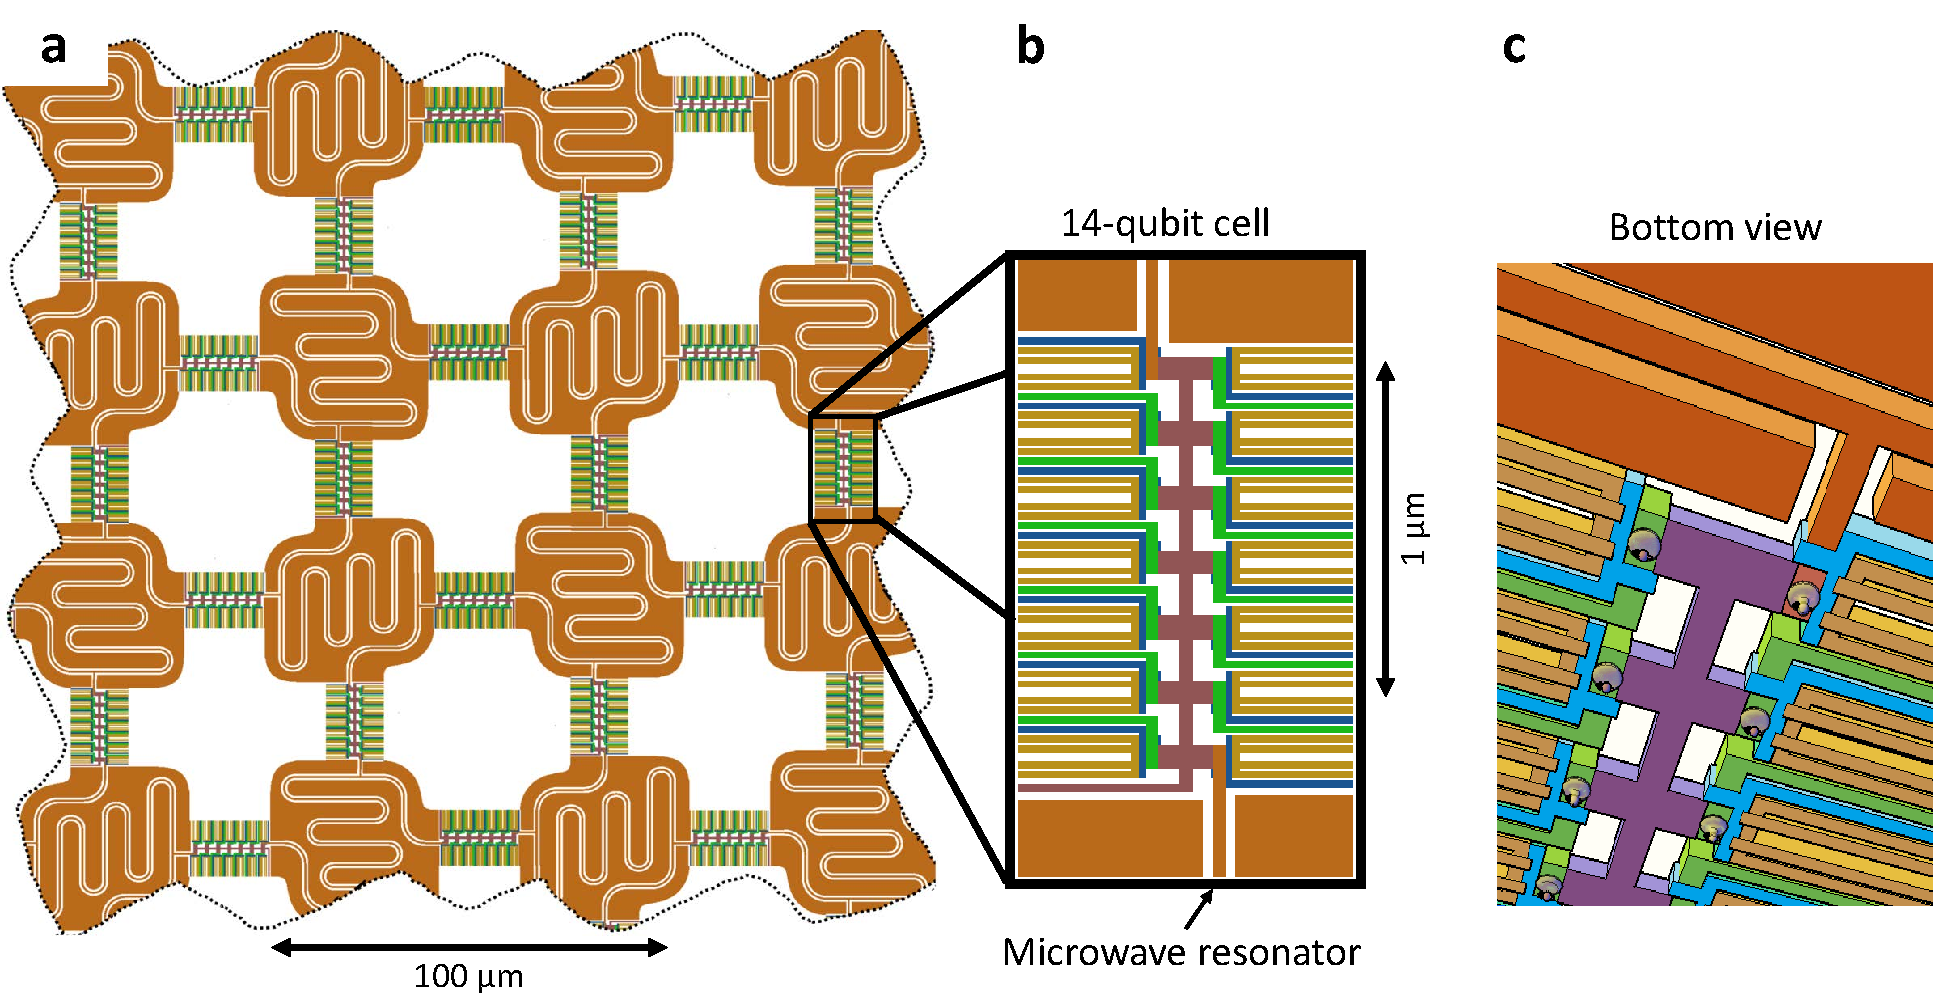
\includegraphics[width=\textwidth]{polished/qp_resonator.pdf}
	\caption[Hybrid quantum processor compatible with current university fabrication standards]{\textbf{Hybrid quantum processor compatible with current university fabrication standards}. Schematic view of a semi-large scale quantum processor which is feasible to build with current fabrication standards in our laboratory. \textbf{a} shows the processor where multiple 14-qubit cells are connected by superconducting resonators to a large computer. \textbf{b} shows the 14-qubit cell in detail from the top while \textbf{c} shows a bottom view. 14 flip-flop qubits are connected via nearest-neighbour or next-nearest-neighbour dipole-dipole interaction. Electrons can be loaded via a central reservoir (purple) and each qubit is read-out via a SET (yellow). The outer-most qubit is coupled to the resonator vacuum field with then allows for coupling to the next 14-qubit cell. }
	\label{fig:qp_14cell}
\end{figure}

Figure \ref{fig:qp_14cell} shows a simple version of a semi-large scale hybrid quantum computer, that only uses current standard 2D university fabrication techniques (see chapter \ref{sec:fabrication}) and could be thus fabricated in our laboratory. It consists out of 14-qubit cells connected by superconducting resonators. While the advantage of this processor is clearly its simplicity, the disadvantage is that parallel operations are very limited and thus quantum error correction cannot be applied as its overhead is too large. However, this processor could be used for small scale proof-of-principle experiments, like running algorithms such as Shor or Joszca-Deutsch \cite{Shor, Joszca}. 

\begin{figure}
	\centering
	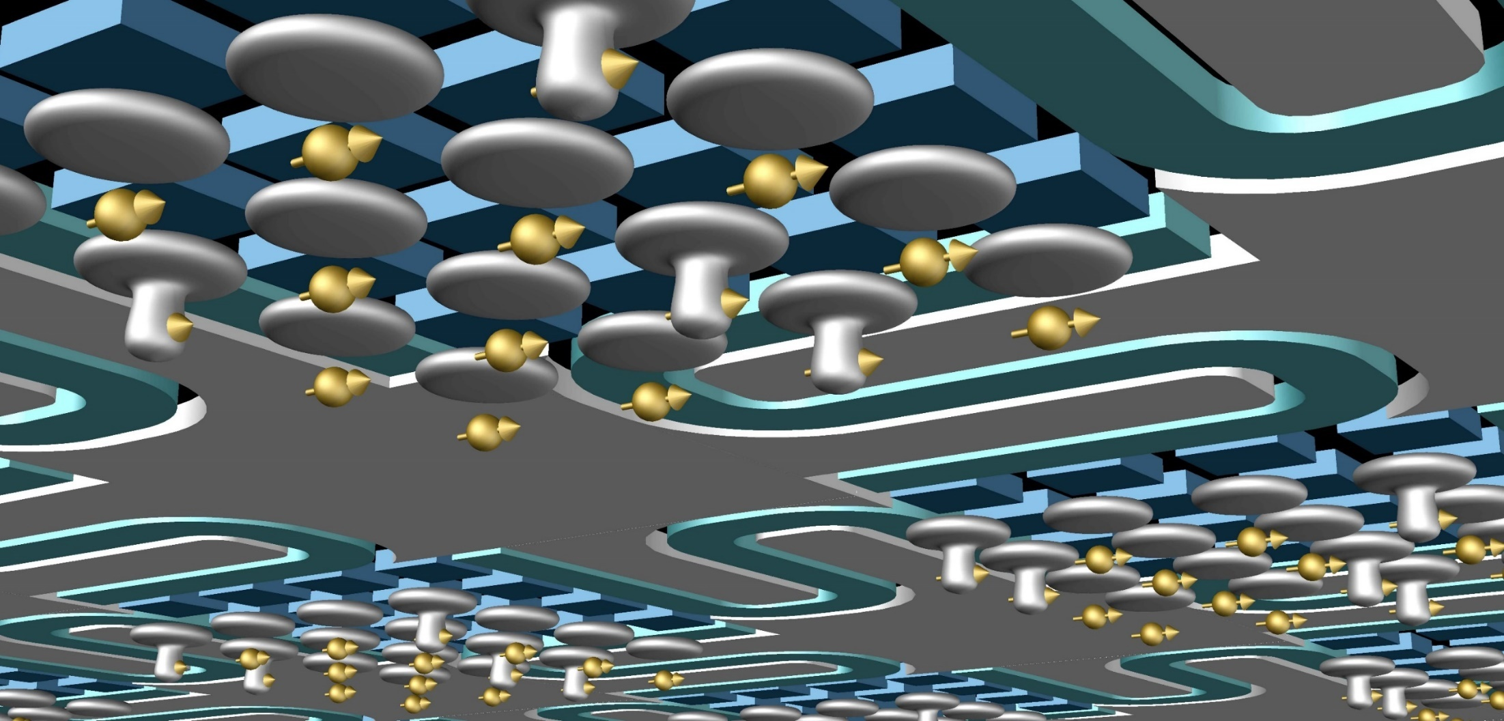
\includegraphics[width=\textwidth]{polished/qp_mixed.png}
	\caption[Large-scale hybrid quantum processor]{\textbf{Large-scale hybrid quantum processor}.
		\textbf{a} Schematic view of a large-scale quantum processor where 2D arrays of 16 dipolar coupled flip-flop qubits are connected via superconducting resonators. The drawing is not to scale; control lines and readout devices are not shown.}
	\label{fig:qp_mixed}
\end{figure}

Figure \ref{fig:qp_mixed} shows a large-scale quantum processor that consists out of 2D arrays of dipolar coupled flip-flop qubits, connected with superconducting resonators. Here, the size of the 2D flip-flop arrays is limited by the space required by read-out and control lines. In this case advanced error-correction codes may be implemented\cite{Knill2005,Nickerson2013,Terhal2015,Li2018a}, but the overhead it still large due to limited parallelism. This type of 2D arrays required 3D CMOS fabrication as the control and read-out lines need to be connected from above or below. 

Ultimately, one wants to build a full 2D array of only flip-flop qubits as presented in figure \ref{fig:qp_surfaceCode} for complete connectability and enhanced parallelism. This architecture allows proper quantum error correction as it is compatible with the surface code\cite{Fowler2012}: Each qubit is surrounded by ancilla qubits to detect errors. The qubits and ancillas interact with their neighbourings via the dipole-dipole interaction and all mutual qubit couplings are tunable and gateable. 

\begin{figure}
	\centering
	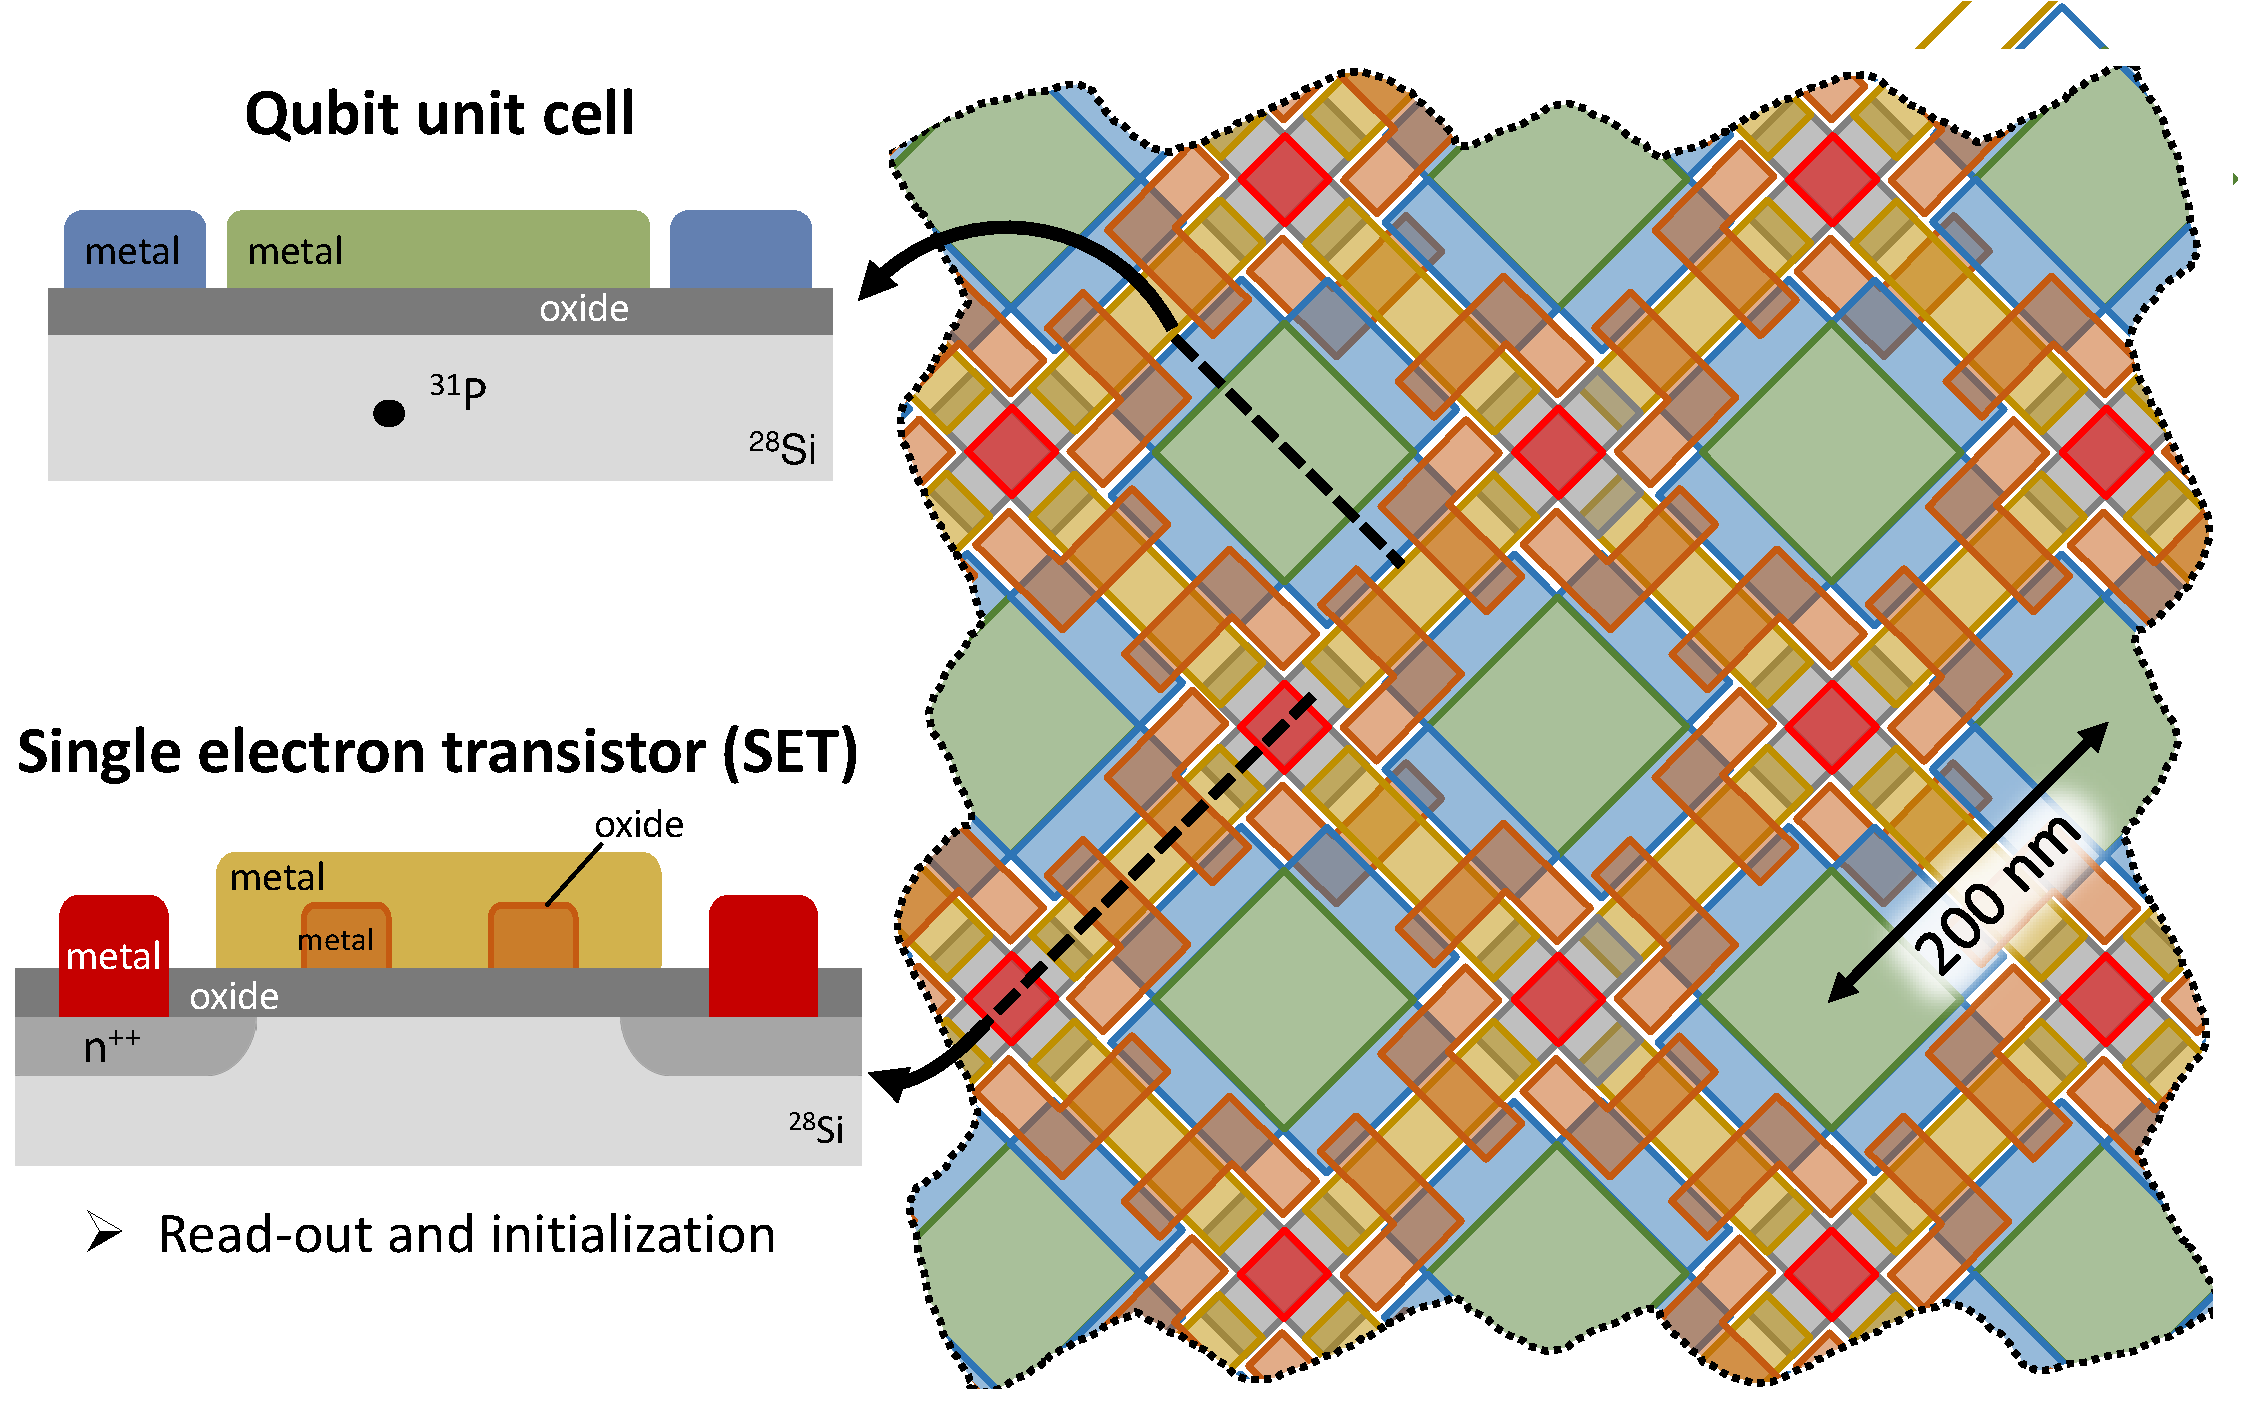
\includegraphics[width=\textwidth]{polished/surfaceCode.pdf}
	\caption[Surface code architecture]{\textbf{Surface code architecture}. Schematic view of a large-scale quantum processor that is compatible with the surface code \cite{Fowler2012}. Qubit unit cells consisting out of donors with a gate stack for tunnel coupling control are coupled via the dipole-dipole interaction. Every other qubit is used as an ancilla. Readout and initialization is performed via a SET. }
	\label{fig:qp_surfaceCode}
\end{figure}



\section{Operation principles of an electrically controlled donor quantum processor}

The fundamental operation principle for our donor quantum processor remains the same for the three suggested implementations. 

For initialization we use the n++ region and either the SET gate stack in Coulomb blockade or a designated reservoir to load an electron onto the donor. 
Idle qubits have electrons either at the interface or the donor, leaving them completely uncoupled to other qubits. Electrons are then adiabatically shifted towards the donor ionization point for quantum operations (see chapter \ref{sec:adiabatic_pc} and \ref{sec:elecDrive}).
Qubit read-out can be obtained by spin-dependent tunnelling into a cold charge reservoir, detected by a single-electron transistor \cite{Morello2010}. Read-out times can be $\sim1~\mu$s with cryogenic amplifiers \cite{Curry2015}, which is comparable to the time necessary to perform, for example, $\sim 20$ individual gates lasting $\sim 50$~ns each, in a surface code error correction protocol \cite{Fowler2012}.

\section{Nuclear qubit based processor}

Instead of flip-flop qubits, nuclear qubits can be used in the quantum processor. These have the advantage of having record coherence times $T_2 \gtrsim 30$~s (ref. \cite{Muhonen2014}) when the donor is ionization (the electron is at the interface). The magnetic drive can be a global, always-on field, e.g. supplied by a 3D microwave cavity. Quantum information can be swapped between the nuclear and the flip-flop qubit by simply applying an ESR $\pi$-pulse that excites the $\lvert{\downarrow\Downarrow}\rangle$ state to $\lvert{\uparrow\Downarrow}\rangle$ (Fig.~\ref{fig:hfchange}).
 
% Chapter Template

\chapter{Device fabrication and experimental methods} % Main chapter title

\label{Chapter5} 

\HRule
\vspace{0.5cm} \hspace{2cm}
\small
\hangindent=4cm
\\
        ``\emph{Scalability is the future}"
\\ \\
\hangindent=4cm
\begin{flushright}
--? \\
\end{flushright}

\vspace{0.5cm}

\noindent \HRule
\clearpage

\section{Device design} \label{sec:deviceDesign}

To propel the flip-flop qubit from theory to reality, we are using nanofabrication techniques to build the qubit, starting from a blank silicon wafer. We start with inventing designs for both the direct dipole-dipole coupling approach and coupling to a superconducting resonator that fulfil all requirements of the flip-flop qubit and comply with the fabrication tools available to us. 
From chapter \ref{Chapter2} we know what the flip-flop qubit requirements entail: We need to be able to readout the electron state, control the tunnel coupling, confine the electron at the interface and most importantly electrically control the donor both with DC voltages and fast pulses.
Additionally we would like an ESR antenna to be able to perform ESR and NMR on the electron and nuclear spin states separately from any flip-flop control, just like in a standard donor qubit device.  The following section describes how these requirements can be implemented for direct dipole-dipole coupling while section \ref{sec:designCPWR} discusses the resonator approach. 

\subsection{Flip-flop qubit} \label{sec:designFF}

\begin{figure}
	\centering
	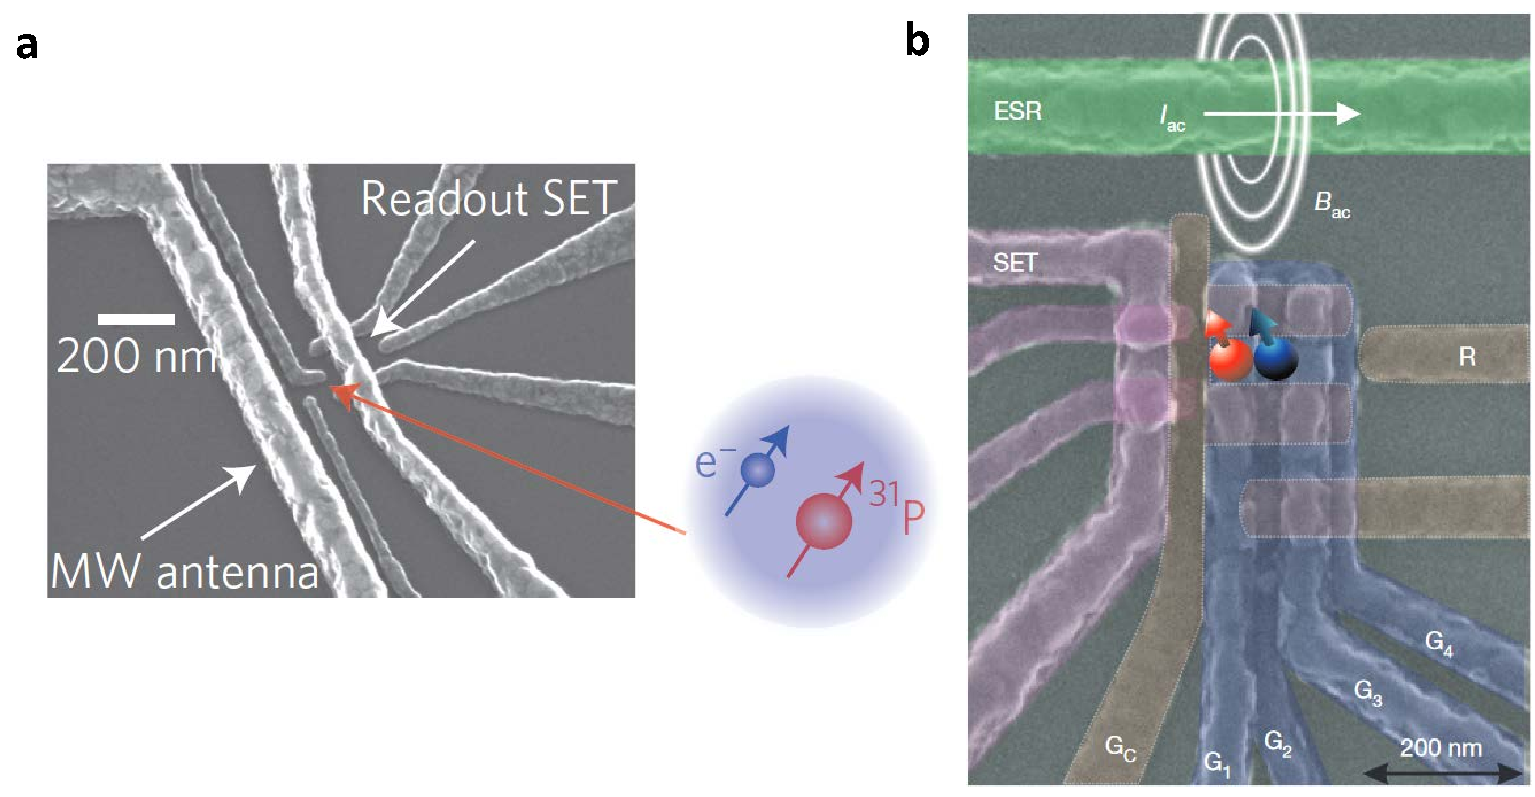
\includegraphics[width=0.8\textwidth]{polished/donorDot.pdf}
	\caption[Silicon donor and quantum dot qubit designs]{\textbf{Silicon donor and quantum dot qubit designs. a} Scanning micrograph of a typical phosphorus donor device in silicon. Both the electron and the nucleus can be operated as a qubit in this device structure \cite{Muhonen2014}. \textbf{b} Scanning micrograph of a typical CMOS quantum dot device in silicon which can be operated as a single or double quantum dot qubit \cite{Veldhorst2014}.}
	\label{fig:donorDotDevices}
\end{figure}

\begin{figure}
	\centering
	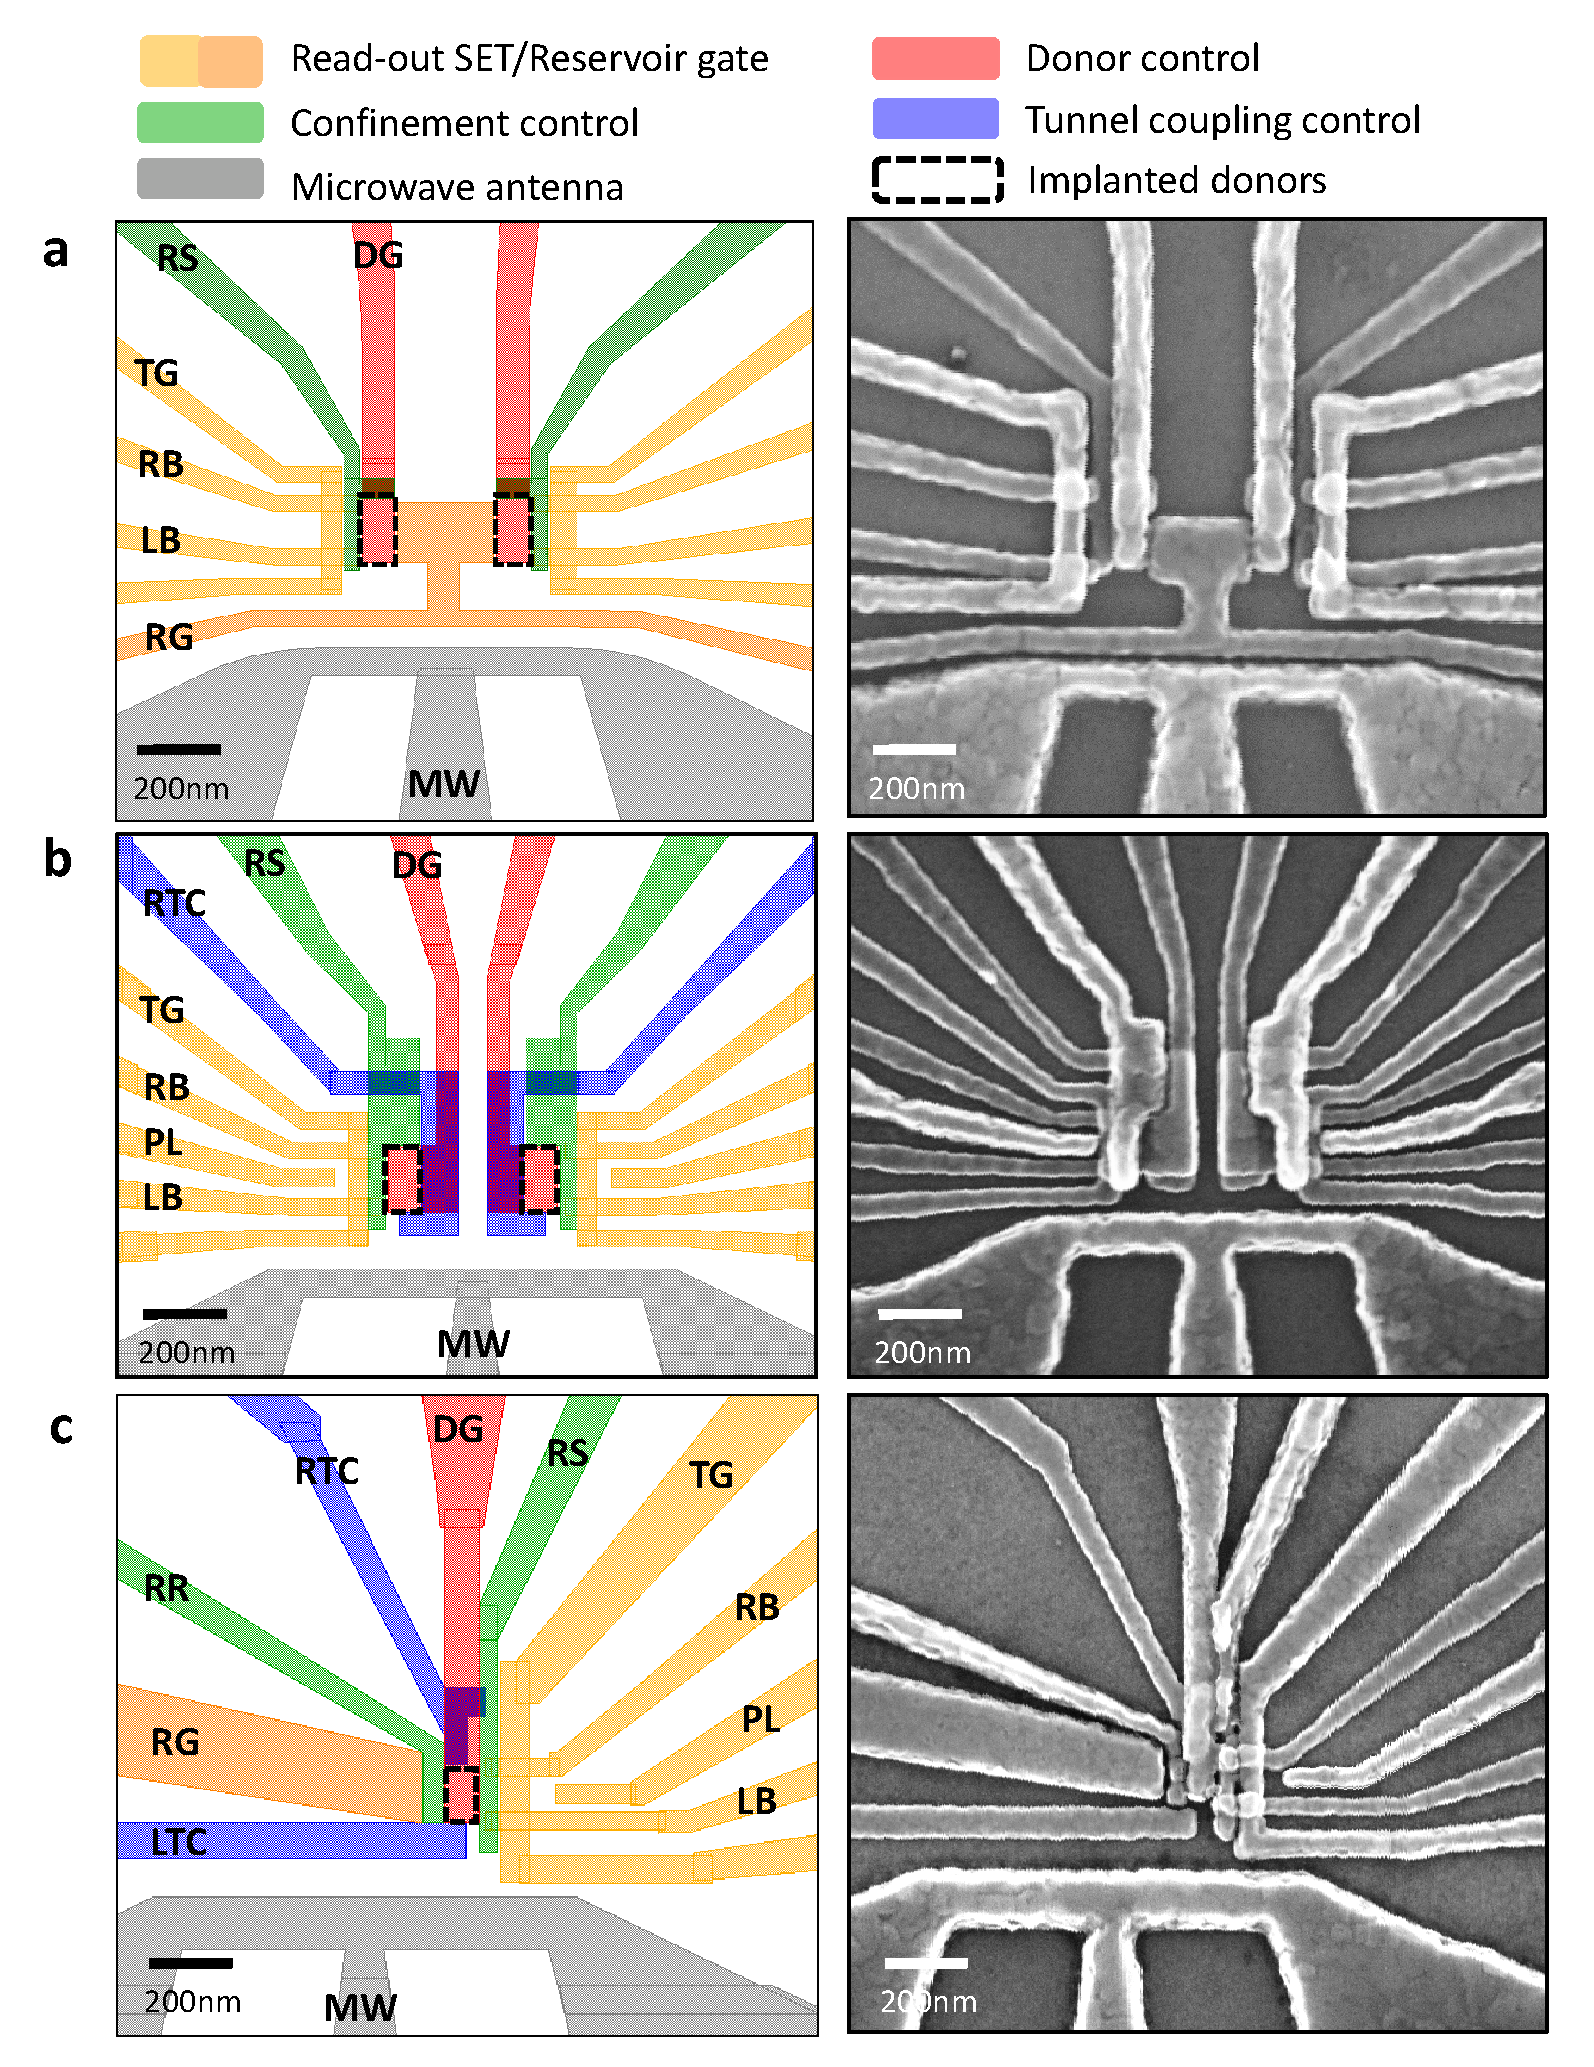
\includegraphics[width=\textwidth]{polished/FF_designs2.pdf}
	\caption[Flip-flop qubit designs for direct dipole-dipole coupling]{\textbf{Flip-flop qubit designs for direct dipole-dipole coupling. } The left column shows the flip-flop qubit design color-coded with gate purpose and gate labels while the right column shows the corresponding scanning micrograph of the finished devices. \textbf{a} Two-qubit flip-flop design with electron confinement control and reservoir for ease of readout. The confinement gate (RS, green) can also be used to modify the tunnel coupling within the voltage range set by the readout parameters. \textbf{b} Two-qubit flip-flop design with extended tunnel coupling control (RTC, blue). A plunger gate (PL, yellow) was added for increased adjustability of the SET. However the additional reservoir was removed. \textbf{c} Single flip-flop qubit device with full tunnel coupling control and readout adjustability.}
	\label{fig:designFF}
\end{figure}

We base our flip-flop qubit structure on existing donor and quantum dot structures (Fig.  \ref{fig:donorDotDevices}) that have made our research teams at UNSW very successful over the last decade \cite{Muhonen2014, Veldhorst2014}. We are working with donors in silicon but also separate the electron from the donor and confine it at the silicon interface - just like a quantum dot. Thus our flip-flop qubit will be a hybrid structure from the donor design shown in figure \ref{fig:donorDotDevices}a and the quantum dot design in figure \ref{fig:donorDotDevices}b. The first generation design of the flip-flop qubit is pictured in figure \ref{fig:designFF}a with a color-coded  layout on the left and an scanning micrograph image on the right. 

The key elements prominent in both donor and dot devices remain unchanged: We use a SET for electron readout (yellow), consisting out of two barriers ("right barrier" - RB, "left barrier" - LB) and a top gate (TG) with contact to a positively doped region ("source" - S and "drain" -D) (see section \ref{sec:qubit_initMeas}). Moreover we employ a coplanar microwave antenna (MW, grey) to supply microwave and radio frequency magnetic fields (see section \ref{sec:qubit_control}). 
We add a gate between the donor and the SET ("rate gate SET" - RS, green), like in the QD devices, to control the tunnel rate of the electron to the SET and prevent escape of the interface state. Additionally this gate can be used to tune the tunnel coupling. Most importantly we add an impedance matched gate on top of the donor to control the donor state and send fast electric pulses ("donor gate" - DG, red). 
However, we encounter one problem: To tune the tunnel coupling significantly we need to pull the electron horizontally by up to $100\,$nm. Consequently we choose an implantation window size of $60\times120\,$nm as indicated in figure \ref{fig:designFF}. Together with the necessary SET rate gate, this can lead to distances of the donor to the SET island of over $100\,$nm - too far for significant electron tunnelling for readout. To account for this difficulty we add an additional reservoir ("reservoir gate" - RG, orange, "reservoir source" - R). This brings two distinct advantages: Firstly, any donor close to either the SET island or the reservoir can be read out with the traditional donor readout (see section \ref{sec:qubit_initMeas}). Secondly, if the dot cannot be readout from the donor, we can readout the interface (quantum dot) state instead. Therefore we bias the donor such that the dot state becomes favourable, as shown in figure \ref{fig:ff_readout}. However, to avoid the electron from just escaping to the reservoir, we need to adjust the Fermi level of the reservoir such that the dot state lies below and will be occupied. During this process the SET Fermi level stays constant to provide charge sensing. 
We mirror this one-qubit structure at a distance of $200\,$nm to achieve a two-qubit device.

\begin{figure}
	\centering
	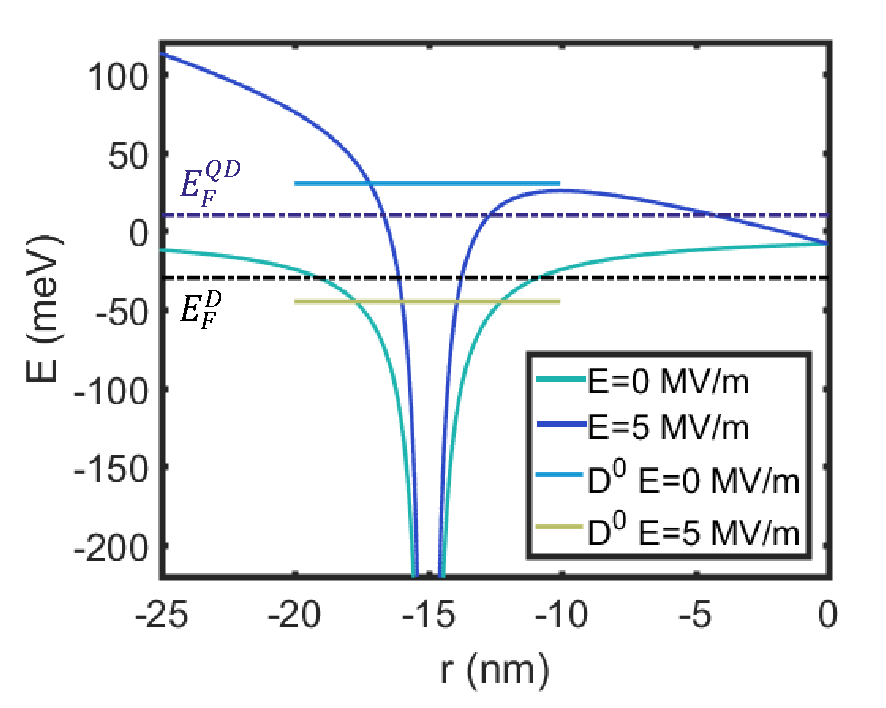
\includegraphics[width=0.8\textwidth]{polished/ff_readout.pdf}
	\caption[Flip-flop qubit readout energy diagram]{\textbf{Flip-flop qubit readout energy diagram. } Coulomb energy of the donor without and with an electric field of $5\,$MV/m applied. The $D_0$ donor ionization energy is $45.6\,$mV. At $r=0\,$nm the SiO$_2$ interface is positioned. The dotted lines show the reservoir Fermi level adjusted for an occupied donor (black) and dot state (blue). }
	\label{fig:ff_readout}
\end{figure}

In the following a few alternative, improved versions of this basic flip-flop structure are presented. Figure \ref{fig:designFF}b shows generation two where we added a plunger gate (PL, yellow) for better SET adjustment and an additional tunnel gate ("right tunnel coupling gate" - RTC, blue) to have higher control over the tunnel coupling, but at cost of the reservoir gate. 
Generation three (Fig. \ref{fig:designFF}c) incorporates both high tunnel coupling control with another tunnel coupling control gate added ("left tunnel coupling gate" - LTC, blue) and high adjustability for electron readout in form of an additional reservoir (RG), two rate gates ("rate gate reservoir" - RR and RS, green) and a plunger gate (PL). To achieve this highly controllable device however we had to sacrifice the second qubit. Thus this generation's focus will be one-qubit performance.
A few additional small design changes to be noted are: The SET rate gate as well as the plunger gate have been moved further away from the SET top gate to reduce the effect of strain on the 2DEG below the SET as this can prevent turn-on. Furthermore, the microwave short has been increased in both width and thickness to make it less susceptible to melting from sudden voltage fluctuations. 

\subsection{Coplanar waveguide resonator} \label{sec:designCPWR}

\subsubsection*{Simple resonator qubit design} \label{sec:simple_res_design}

\begin{figure}
	\centering
	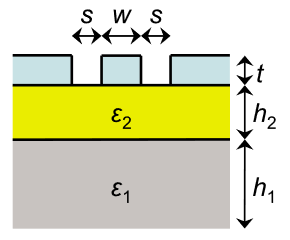
\includegraphics[width=0.4\textwidth]{polished/CPWR.png}
	\caption[Coplanar waveguide resonator geometry]{\textbf{Coplanar waveguide resonator geometry}. Geometric dimensions determining the impedance of a coplanar waveguide resonator.  }
	\label{fig:geometryCPWR}
\end{figure}

To couple our flip-flop qubit to a single photon we use a standard coplanar waveguide resonator (CPWR). This geometry consists out of a central conductor with a ground plane on either side. A cross section is shown in figure \ref{fig:geometryCPWR}. The waveguide width and gap size are chosen for an impedance of $50\,\Omega$ to $w=20\,\mu$m and $s=12\,\mu$m (factor $s/w=0.6$). The parameters are $\epsilon_{1}=11.6$, $h_1=500\,\mu$m for the silicon wafer, $\epsilon_2=3.78$, $h_2=8\,$nm for the silicon oxide layer and $t=50\,$nm for the superconducting film thickness  \cite{Jani2018}. 

We like to operate at a frequency $f_r\gg k_B T/h\approx 400\,$MHz to reduce thermal population, choosing $f_r\approx 6\,$GHz to keep component costs low.  We operate the fundamental mode of a $\lambda/2$ resonator which determines the resonator length to $l=c_0/2\sqrt{\epsilon_{\rm eff}\epsilon_0}\cdot f_r$. $\epsilon_{\rm eff}$ is the effective permittivity of the wave guide which can be estimated to $\epsilon_{\rm eff}=(1+\epsilon_1)/2=6.3$ \cite{PalaciosLaloy2010}. Figure \ref{fig:designCPWR}a shows the CPWR design. 

\begin{figure}
	\centering
	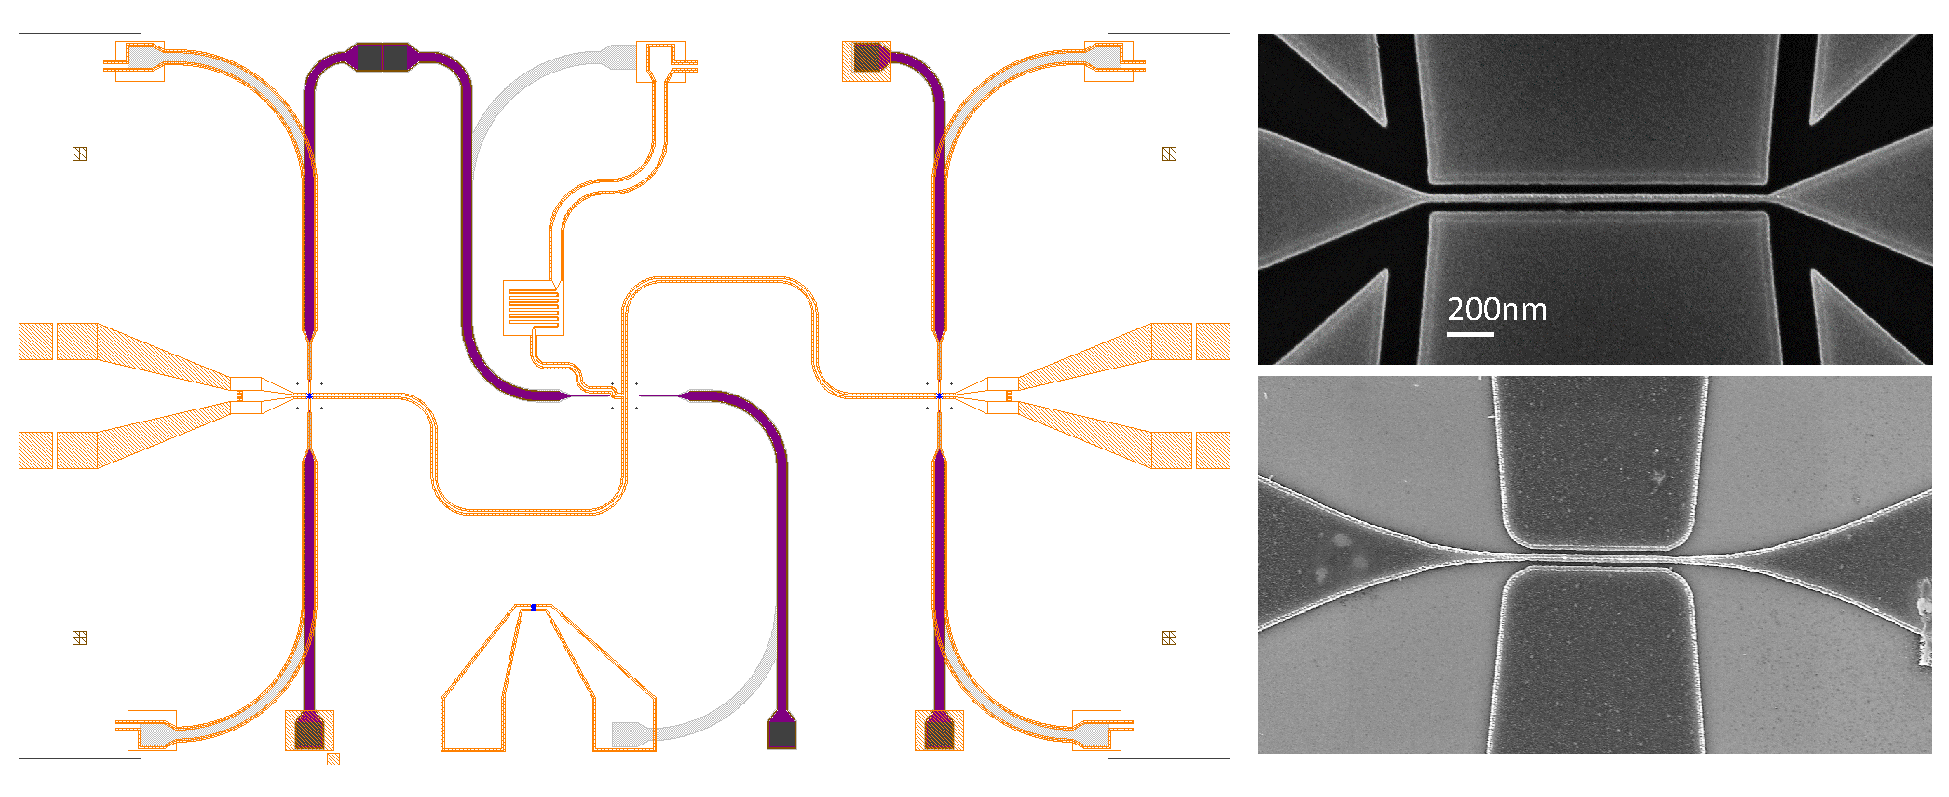
\includegraphics[width=\textwidth]{polished/CPWR_designs.pdf}
	\caption[Simple CPWR qubit design]{\textbf{Simple CPWR qubit design. a} Overview of the CPWR design, color-coded with feature purpose. The sample is covered in a superconducting film with etched regions indicated in orange and green. Purple shows the n+regions with their respective Ohmic contacts in black. The active qubit region, the capacitors and the inductor are shown zoomed-in in \textbf{b} to provide details. \textbf{b} Inductor and capacitor example designs and active qubit region with gate labels. \textbf{c} Scanning micrograph overview of the CPWR. \textbf{d, e} Scanning micrograph of the active qubit region for two different designs. }
	\label{fig:designCPWR}
\end{figure}

The coupling of the resonator to the lines is determined by the capacitor design at each end of the resonator, acting as a semi-reflecting mirror, introducing a strong impedance mismatch. We are aiming for the over-coupled regime where the coupling exceeds the internal losses. We simulate the capacitor size in the computer simulation theory (CST) microwave studio. Ultimately however, we rely on testing different designs as we are operating in the single photon regime where the coupling strength is mainly determined by quantum tunnelling. Figure \ref{fig:designCPWR}b shows an example capacitor design. As we are working in transmission mode we place one capacitor at each end of the resonator. 

Now we integrate our spin qubit into the resonator design by placing several phosphorus donors directly beneath the resonator central conductor (CC). However, we require a vacuum electric field amplitude of $E_{\rm vac}\approx 30\,$V/m to achieve high qubit-resonator coupling rates (see chapter \ref{sec:cqed_ff}, \cite{Tosi2017}). These electric field amplitudes can be reached by narrowing the central conductor in the active qubit region to around $100\,$nm as shown in figure \ref{fig:designCPWR}b \cite{Samkharadze2016}. In order to load electrons to the donors, we incorporate two reservoir gates ("top top gate" - TT and "bottome top gate" - TB) with respective n+ regions and Ohmic contacts ("source" - S and "drain" - D) for each active region which have the ability to bring a 2DEG close to the qubit.

 Finally, we need to apply a bias to the qubit to move the electron. Thus we have to bias the center conductor. Therefore we add a DC feed line at the electric field node at the center of the resonator. High frequency noise is filtered with an on-chip inductor as shown in figure \ref{fig:designCPWR}a,b. 
 
Figure \ref{fig:designCPWR}c-e shows scanning micrographs of the fabricated resonator devices. 

Due to the large metallic ground plans involved in this design, electrostatic discharge (ESD) can be a serious problem with charges accumulating on the metal during fabrication and chip handling. Consequently we removed tips channelling voltage as in figure \ref{fig:designCPWR}d (improved design in figure \ref{fig:designCPWR}e) and grounded all gates to the large ground planes by leaving small strips of metal unetched. After a device has been mounted to an enclosure (see section \ref{sec:packaging}) and all gates are grounded, these strips can be disconnected by scratching with a diamond-tip pen or scriber. 

\subsubsection*{Advanced resonator qubit design} \label{sec:adv_res_design}

While the design presented in the previous section is proficient to operate a flip-flop qubit in its most basic functionality with a bit of luck in the donor position and depth (see chapter \ref{sec:res_chargequbit}), its qubit control capability is very limited. The reservoir gates allow biasing, however they are far away from the qubit due to fabrication limitations (see chapter \ref{sec:fab_cpwr}) and thus wave function control will be very limited if not impossible. Furthermore, many electrons can be loaded under the central conductor during qubit loading. 
To mitigate these issues we are developing a design both more robust against implantation uncertainties as well as allowing higher qubit control. Figure  \ref{fig:designCPWR_new}) shows the current advanced design.  

\begin{figure}
	\centering
	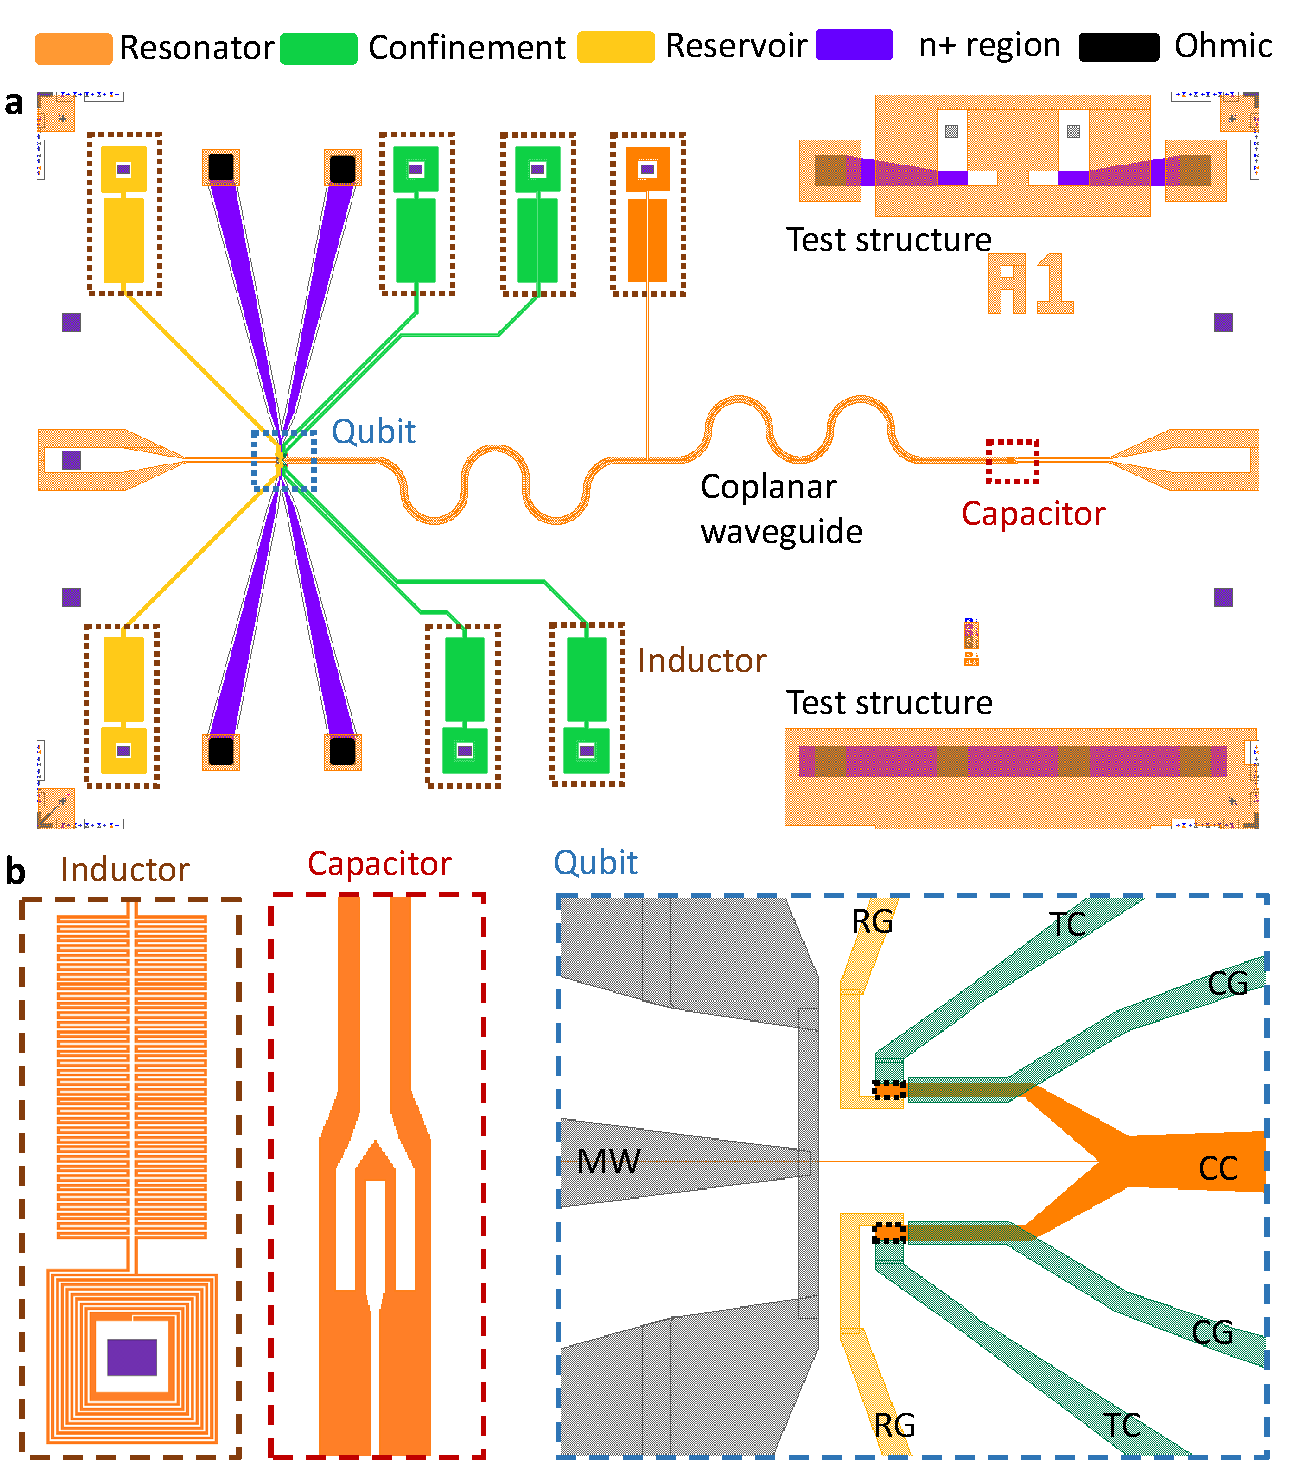
\includegraphics[width=0.9\textwidth]{polished/CPWR_VS.pdf}
	\caption[Advanced CPWR qubit design]{\textbf{Advanced CPWR qubit design. a} Overview of an advanced resonator flip-flop qubit structure, color-codes with feature purpose, which includes several control gates and is operated in reflection. \textbf{b} Detailed view of example inductor and capacitor as well as the active qubit region with gate labels.   }
	\label{fig:designCPWR_new}
\end{figure}

The main difference between the advanced and the simple design is that now we use a two-layer Aluminium structure in the active qubit region (Fig. \ref{fig:designCPWR_new}c), allowing for a much smaller feature size and a more complex gate layout. Furthermore we now operate the resonator in reflection. We have only one active region but fit two qubits inside it. Both have a separate reservoir ("reservoir gate" - RG, yellow) as well as two gates to confine the electron and control tunnel coupling ("tunnel coupling gate" - TC and "confinement gate" - CG, green). Each of these gates has its own on-chip inductor to allow for loss-less DC biasing. We also incorporate a microwave antenna into our design to allow for individual electron and nuclear spin control. 

\section{Device fabrication} \label{sec:fabrication}

\subsection{Silicon wafer} \label{sec:fabWafer}

\begin{figure}
	\centering
	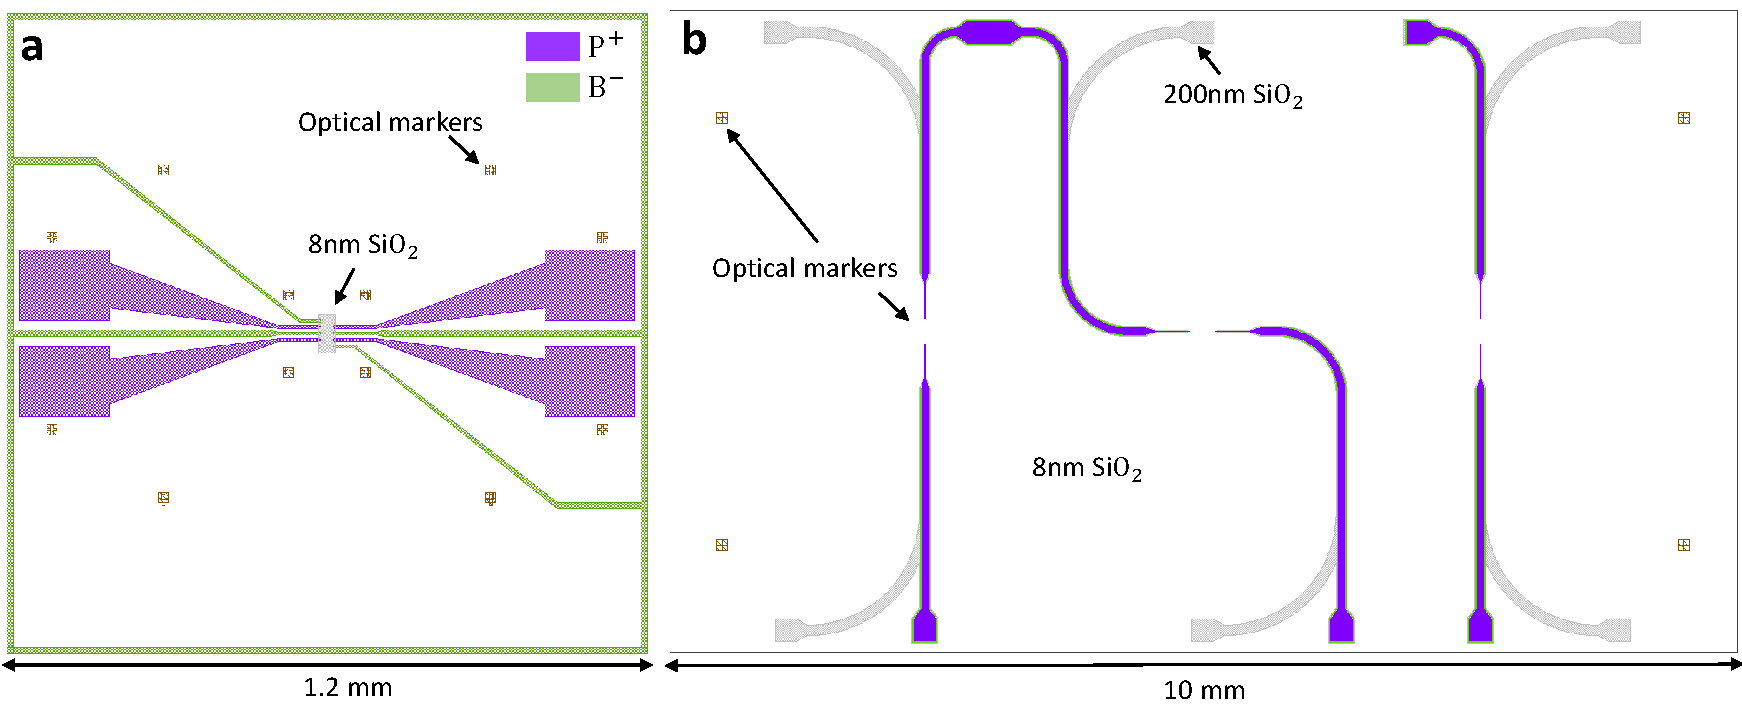
\includegraphics[width=\textwidth]{polished/stock.pdf}
	\caption[Silicon wafer layout]{\textbf{Silicon wafer layout.} Layout of the features patterned on the silicon wafer during wafer preparation for the standard Aluminium devices (\textbf{a}) and the resonator devices (\textbf{b}). 
	%n+ and p+ regions are created with phosphorus and boron diffusion respectively (purple, green). A thin and a thick silicon oxide is grown and optical markers are etched and evaporated
	 }
	\label{fig:wafer}
\end{figure}

All devices start off as a bare silicon wafer. For testing, natural silicon wafers with low residual p-type background doping ($\sim 10^{12}\,\rm{cm}^{-3}$) are used, while highly precise qubit experiments are performed on wafers with an $800\,$nm epitaxial layer of isotopically purified $^{28}$Si on top of $500\,\mu$m thick high purity natural silicon, provided by K. Itoh. The $^{28}$Si has a residual concentration of $730\,$ppm of $^{29}$Si and $30\,$ppm $^{30}$Si.

The first step after acquiring a new wafer is a thorough clean. Then optical alignment marks are etched into the silicon. Next the wafers are doped firstly with Boron ($B^-$) to create positively charged guard rings. These guards prevent leakage at the Si-SiO$_2$ interface when positive charges trapped in the wet field oxide induce an unintentional two-dimensional electron gas (2DEG). Then phosphorus ($P^+$) is diffused to create $n+$ regions to form the source and drain contacts. Afterwards $200\,$nm of field oxide are grown in a wet thermal oxidation furnace. Next, the field oxide is removed in the active qubit region to be replaced by a $8\,$nm ($2\,$nm for CPWR style devices) of high quality gate oxide, grown in an ultra-dry furnace. Lastly micrometer sized markers formed out of Platinum on top of Titanium (TiPt markers) are patterned for course alignment with electron beam lithography (EBL). Figure \ref{fig:wafer}a shows an the design of a standard qubit wafer after this initial processing. 

The processing of wafers designated for coupling to superconducting resonators is done in the same way. The only noticeable difference is that most of the wafer is the active region and thus only where the top gates are indented, a thick field oxide is grown. This wafer design is shown in figure \ref{fig:wafer}b. 


\subsection{Nano-fabrication process - standard aluminium devices} \label{sec:nanofab_al}

Once the silicon wafers have been prepared, they are diced into smaller chips for different projects. While all silicon donor aluminium style devices use inherently a very similar fabrication process, small differences occur due to individual preferences and cleanroom superstition. In the following the process specific to the flip-flop qubit used by the author in this thesis is presented. 

\paragraph*{Cleaning}
To remove any residue of resist or other contaminants the chips are cleaned by soaking them first in acetone and subsequently in Isopropyl alcohol (IPA) for each 10 min while applying ultrasound. The cleaning process is finished with 10 min of oxygen plasma ashing. 

\begin{figure}
	\centering
	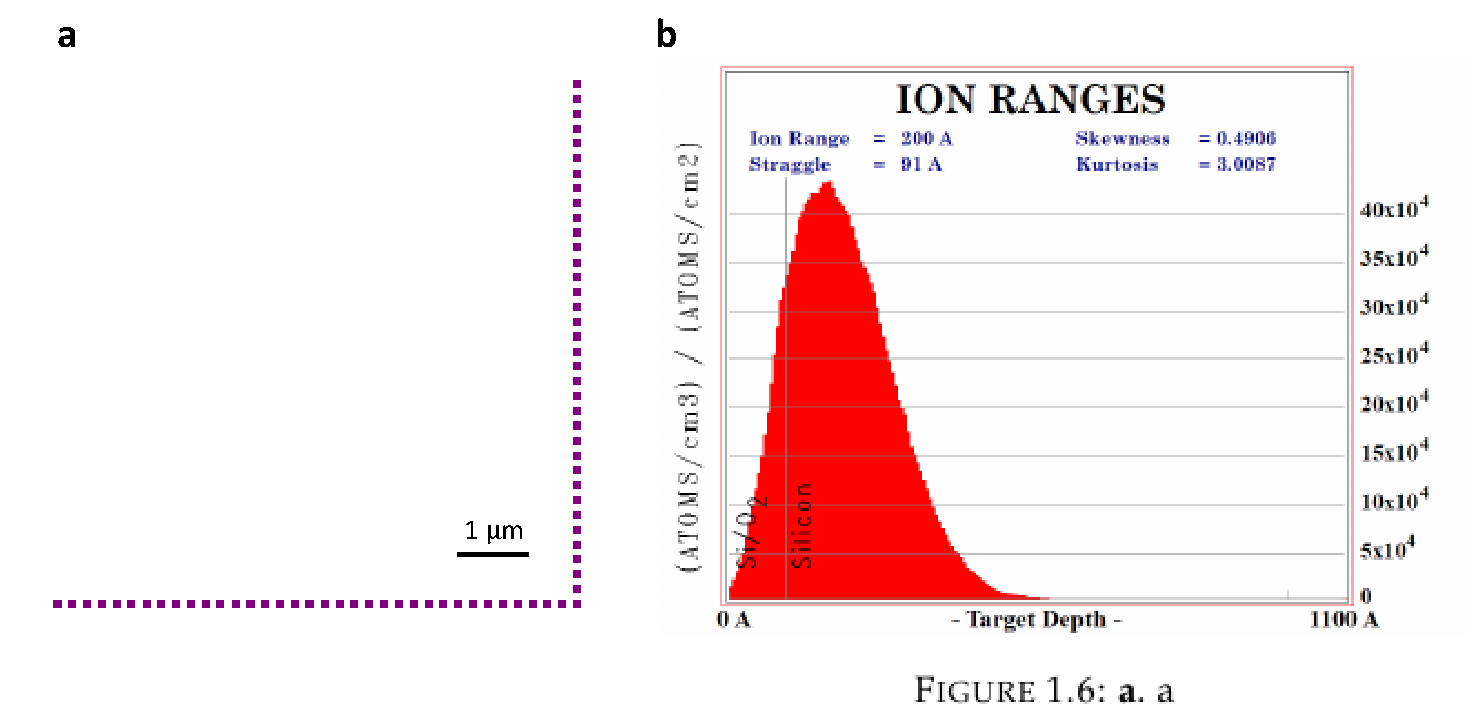
\includegraphics[width=0.9\textwidth]{polished/implantion_TiPtmarks.pdf}
	\caption[TiPt marker design and ion distribution for implantation]{\textbf{TiPt marker design and ion distribution for implantation a.} Design of the nanometric TiPt markers used for EBL alignment of the different layers. The individual square design is robust against melting during RTA. \textbf{b} Distribution of ions with depth for an acceleration voltage of 12keV of P$^+$ ions with a fluence of $2\cdot10^{11}$/cm$^2$.   }
	\label{fig:TiPtmarks_impl}
\end{figure}

\paragraph*{TiPt markers}
The first processing step is the formation of the nanometric markers in each pixel which enable alignment of different layers during EBL. These markers need to withstand temperatures of $1000\,\degree$C during subsequent processing steps. Therefore we use Platinum which not only has a very high melting point of $1763\,\degree$C but also has a high atomic number resulting in good contrast on the electron beam microscope. For adhesion to the silicon oxide surface we add a thin layer of Titanium with a melting point of $1668\,\degree$C. Regardless of these high melting points, large TiPt structures melt and deform. Consequently we use marker shapes consisting out of many small $100\times100\,$nm squares as shown in figure \ref{fig:TiPtmarks_impl}a which survive our high temperature process. 
We create these markers using EBL.

\textit{Standard EBL process:} We first bake our chip at $180\,\degree$C for 10 min and then spin polymethyl methacrylate (PMMA) A4 resist with $4000\,$rpm for 40s with 10s of $8000\,$rpm finish. This gives a resist thickness of $200\,$nm. The resist is then baked for 90s at $180\,\degree$C. Droplets of colloidal gold solution can be placed on the corners of the chip as focus markers. The pattern is written with a RAITH150-Two EBL system with an acceleration voltage of $30\,$keV and a dose of around $500\mu C/cm^2$, depending on aperture, feature size and geometry. After exposure, the resist is developed for 40s in a 1:3 solution of methyl-sobutyl-ketone (MIBK) and IPA and for 20s in IPA with a 5s ultrasound finish. 
Subsequently 15nm of Titanium and 65nm of Platinum are evaporated by electron beam physical vapour deposition (EBPVD). Then the chip is placed in N-methyl-2-pyrollidone (NMP) at $80\,\degree$C for 5min to perform lift off. 

\paragraph*{Donor implantation}
The next step is the implantation of our phosphorus donors. Therefore a PMMA mask of dimensions  $120\times60\,$nm is patterned with EBL in each pixel ("implantation window"). We require a donor depth of around 10-15nm below the silicon oxide. As the tunnel coupling between the donor and dot can be reduced but not increased we aim for 10nm. An acceleration voltage of 12keV of $P^+$ ions complies with this requirement as the simulated ion depth distribution in figure \ref{fig:TiPtmarks_impl}b shows. We'd like 8-10 donors in our implantation window which corresponds to a fluence of $2\cdot 10^{11}/cm^2$ and an average donor distance of 25nm. The implantation is performed by Jeff McCallum. After the implantation is completed the resist is removed and the chip undergoes rapid thermal annealing (RTA) for 5s at $1000\,\degree$C. This activates the donors and repairs the damage caused in the silicon lattice by the ion implantation \cite{McCamey2005}. 

\paragraph*{Ohmic contacts}
Finally Aluminium Ohmic contacts to the diffused $n+$ regions are formed and activated with a forming gas anneal (FGA) (N$_2\ 95\%$, H$_2\ 5\%$) at $400\degree$C for 15min in the clean anneal furnace and the chip is diced into 4x4 pixel pieces for individual processing. 

\paragraph*{Multi-layer Aluminum nanostructures}

\begin{figure}
	\centering
	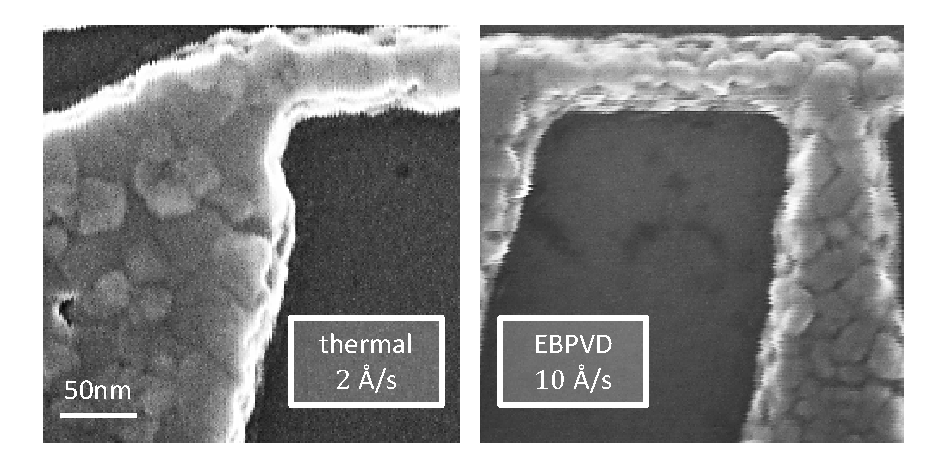
\includegraphics[width=0.7\textwidth]{polished/grainsize.pdf}
	\caption[Aluminium grain size for thermal evaporation and EBPVD]{\textbf{Aluminium grain size for thermal evaporation and EBPVD. a} Aluminium structure evaporated at a rate of $2\,\Angstrom$/s in a thermal evaporator. The grains are 30-50nm large. \textbf{b} Aluminium structure evaporated at a rate of $10\,\AA$/s with EBPVD. The grains are 10-30nm large. }
	\label{fig:grainsize}
\end{figure}

On each 4x4 pixel piece three layers of aluminium gates on top and around the implantation window are added. For each layer the piece undergoes the following steps. 
First the piece is cleaned, then PMMA resist is spun and exposed during EBL as described above for the TiPt markers. After development aluminium is evaporated either in a thermal or an EBPVD evaporator. Tests have been performed and we find that the evaporation rate and its stability directly influences the aluminium grain size. Thermal evaporation can be unstable due to a fluctuating current and is restricted to rates below $3\,$\AA/s. Thus it regularly leads to a larger grains than EBPVD where evaporation rates of $10\,$\AA/s can be achieved - see figure \ref{fig:grainsize}. With EBPVD we evaporate 25nm, 45nm and 80nm subsequently for the different layers and lift off in hot NMP for 1.5-3h. During the following oxygen plasma ash and baking, the outer $2-3\,$nm of each aluminium layer are oxidized to form an electrically insulating layer. Figure \ref{fig:ff_layers} shows the layer schematic and each layer individually. 

\begin{figure}
	\centering
	\includegraphics[width=\textwidth]{polished/FF_layers.pdf}
	\caption[Aluminium layer arrangement of the dipole flip-flop qubit]{\textbf{Aluminium layer arrangement of the dipole flip-flop qubit.} Qubit gate layout color-coded for the three layers and corresponding scanning micrograph images for each layer.}
	\label{fig:ff_layers}
\end{figure}

\paragraph*{Finish}
After the last layer has been completed, the piece is cleaned one more time and FGA is performed to passivate any charge traps at the Si-SiO$_2$ interface\cite{Brower1988}.

\subsection{Nano-fabrication process - resonator devices} \label{sec:fab_cpwr}

As our research group had not fabricated any form of superconducting devices before, we started building up a new process which is still undergoing development. This section describes the fabrication performed for the measurements presented in this thesis and gives an outlook for new, more sophisticated resonator devices. 

\begin{figure}
	\centering
	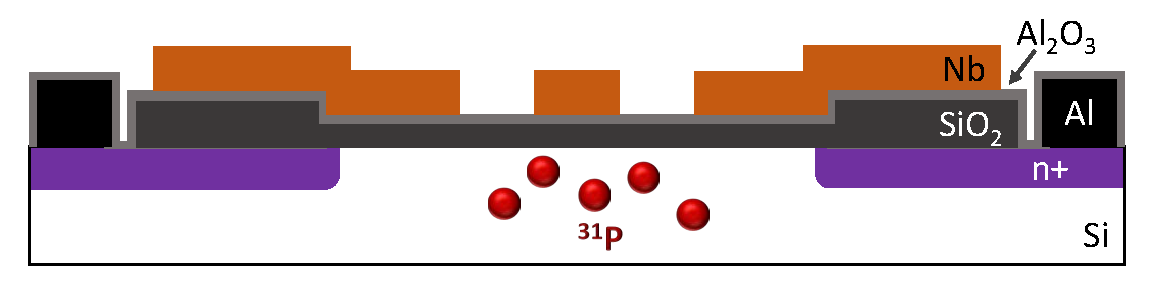
\includegraphics[width=0.9\textwidth]{polished/fab_cpwr.pdf}
	\caption[SEM FF]{\textbf{a}. a }
	\label{fig:fab_cpwr}
\end{figure}

\paragraph*{Cleaning} 
First the wafer is cleaned in the same way as for the aluminium devices. However, once the niobium layer has been deposited, oxygen ashing oxidises the niobium to a degree that compromises the quality of the superconducting film, thus will not be performed.

\paragraph*{Donor implantation}
The next step is the implantation of our phosphorus donors. Therefore a photo mask of dimensions  $44\times24\,\mu$m is patterned with photo-lithography in each pixel (implantation window). We implant $P^+$ ions with an acceleration voltage of 11keV and a fluence of $1\cdot 10^{11}/cm^2$ which corresponds to an average donor distance of 38nm. The implantation is performed by Jeff McCallum. After the implantation is completed the resist is removed and the wafer undergoes RTA. Finally Aluminium Ohmic contacts to the diffused $n+$ regions are formed and activated with a FGA.

\paragraph*{Sputtering}
First we apply a thin layer of Al$_2$O$_3$ to serve as an etch stopper. With atomic layer deposition (ALD) we run 30 cycles at $250\,\degree$C which gives 3 nm. 
Then the wafer is sent to CSIRO at Lindfield where the 50nm of niobium are sputtered. However, the film thickness fluctuates between $30-40\,$nm which is determined with a stylus profilometre. Using a 4-point measurement we find these films to have a resistance of $15\,\Omega$ at room temperature. 

\paragraph*{Resonator structures}
To pattern our resonator structures we spin PMMA resist and expose it with EBL. In contrast to the aluminium style devices, we write what will be removed. Moreover, the resonators are larger than one write field. To create a smooth coplanar waveguide we employ the fixed beam moving stage (FBMS) technique that moves the stage below the beam for the entirety of the device, thus apprehending stitching issues. After patterning we develop the sample. Then we perform hollow cathode reactive ion etching (HC RIE) with a gas mixture of 20sccm CF$_4$ and 10sccm Ar at a pressure of 5Pa with 50W power to remove the Nb not protected by our PMMA mask. This process needs to be carefully calibrated so that after the etch duration the Nb is fully removed but the PMMA mask is still protecting the remaining Nb surface. For this purpose we always add test samples to the process. After etching the sample is cleaned and ready for packaging. 

\paragraph*{Outlook for advanced resonator devices}
The advanced resonator design fabrication deviates in a few important steps. Firstly, we will use NbTiNt instead of Nb, which has a higher critical field, allowing us to operate in a regime with less relaxation of the flip-flop qubit (see chapter \ref{sec:ff_relax}, \cite{Boross2016}). Secondly, the resonator will be patterned with optical lithography using the mask shown in figure \ref{fig:designCPWR_new}a. After etching, we then fabricate the qubit nanostructures like the Aluminium devices described in section \ref{sec:nanofab_al}. 


\section{Device packaging} \label{sec:packaging}

\begin{figure}
	\centering
	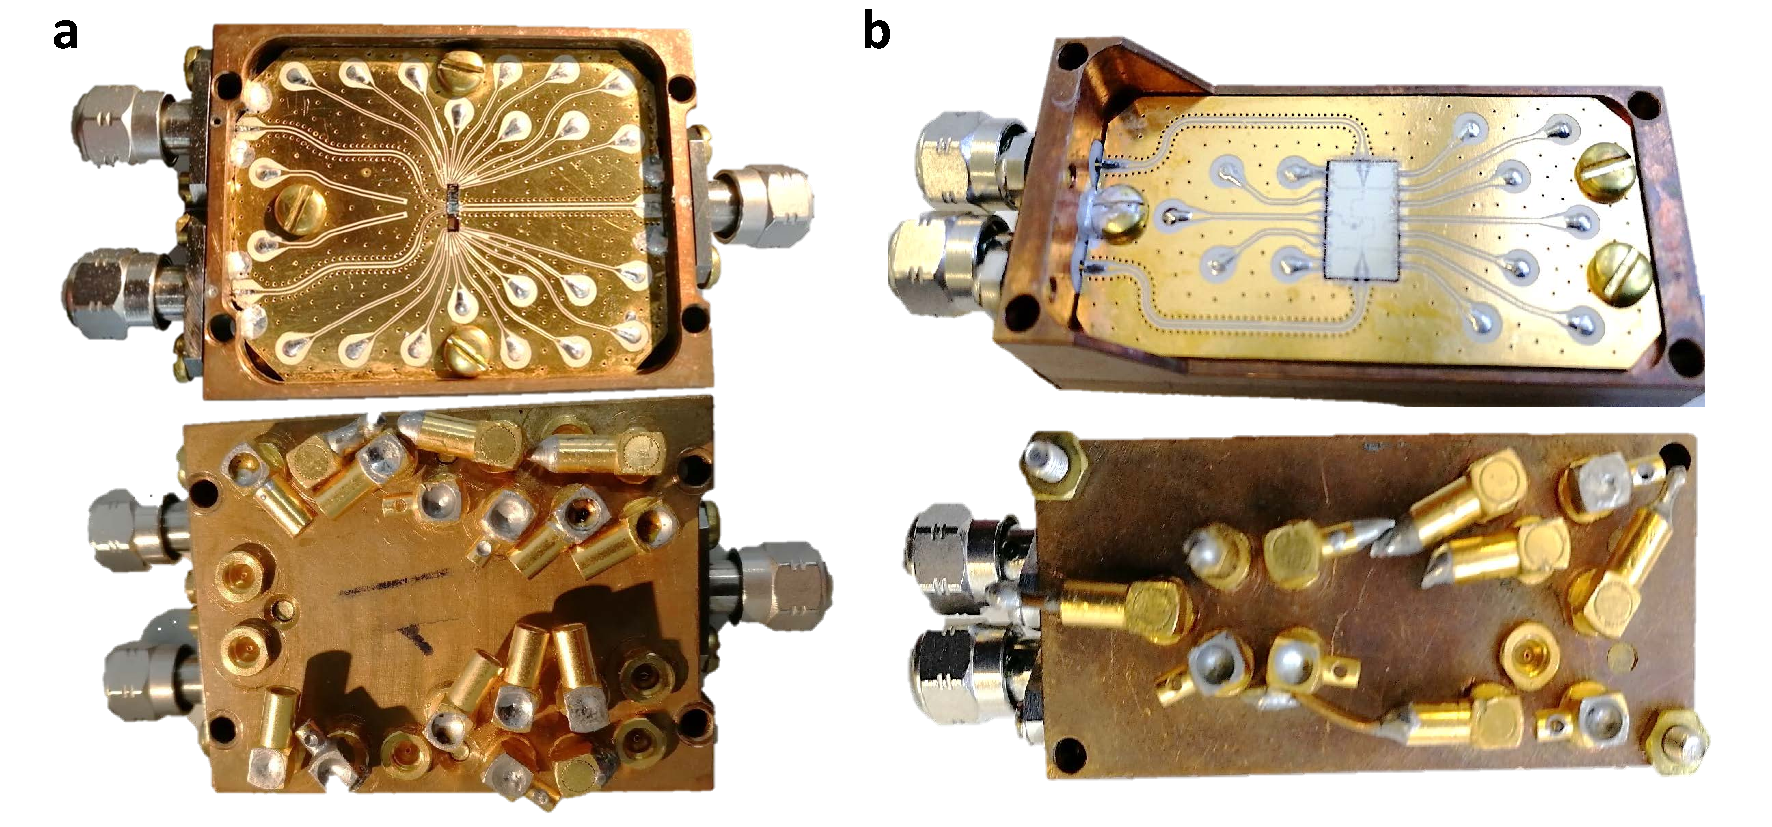
\includegraphics[width=\textwidth]{polished/PCB.pdf}
	\caption[PCB]{\textbf{a}. a }
	\label{fig:pcb}
\end{figure}

To connect our samples to electronics we use a printed circuit board (PCB) inside a copper enclosure as shown in figure \ref{fig:pcb}. These PCBs have been carefully designed with impedance matched lines for all high frequency ports and spare ports to accommodate for design changes. The dipole PCB (Fig. \ref{fig:pcb}a) holds two pixels which makes chip handling slightly easier as the pixel size is only $1.4\times1.4\,$mm. It features two high frequency SMA
and one SK line and 22 MMCX lines. The CPWR PCB (Fig. \ref{fig:pcb}b) holds one pixel and has two SMA and 12 MMCX lines. 

The device is mounted in the PCB opening with PMMA and subsequently connected to the PCB lines with an aluminium wedge wire bonder. Fast frequency lines are bonded as matched as possible by using many short bonds. The CWPR requires many additional bonds (from PCB ground to sample ground and across the different ground sections on the sample) to properly secure the ground plane is equal over the entire chip. During the bonding process all lines remain grounded to avoid electrostatic discharge (ESD) damage. 

\section{Experimental setup} \label{sec:setup}

Our experiments are performed at low temperatures ($\sim 11\,$mK) to prevent spurious thermal excitation as much as possible. Cryogen-free dilution refrigerators (BlueFors LD400 and ??) can achieve these temperatures by  exploiting the enthalpy of mixing of $^4$He and $^3$He. The coldest part of the fridge is where the gases mix and is fittingly called the mixing chamber. There we attach our sample enclosures with our qubits on a cold finger. The fridge is outfitted with a superconducting magnet. The qubit sits in the center of this magnet and thus experiences a homogeneous magnetic field of up to 5 T.

In this thesis three different types of qubits are discussed: the standard electron and nuclear qubit (see chapter \ref{Chapter1} and \ref{Chapter7}), the flip-flop qubit implemented with direct dipole-dipole coupling and resonator coupling (see chapter \ref{Chapter2, Chapter3, Chapter4, Chapter6}). These different qubits have different demands on the measurement setup which will be explained in the following sections. 

\subsection{Electron qubit} \label{sec:setup_en}

\subsubsection{Cables and filtering}

\begin{figure}
	\centering
	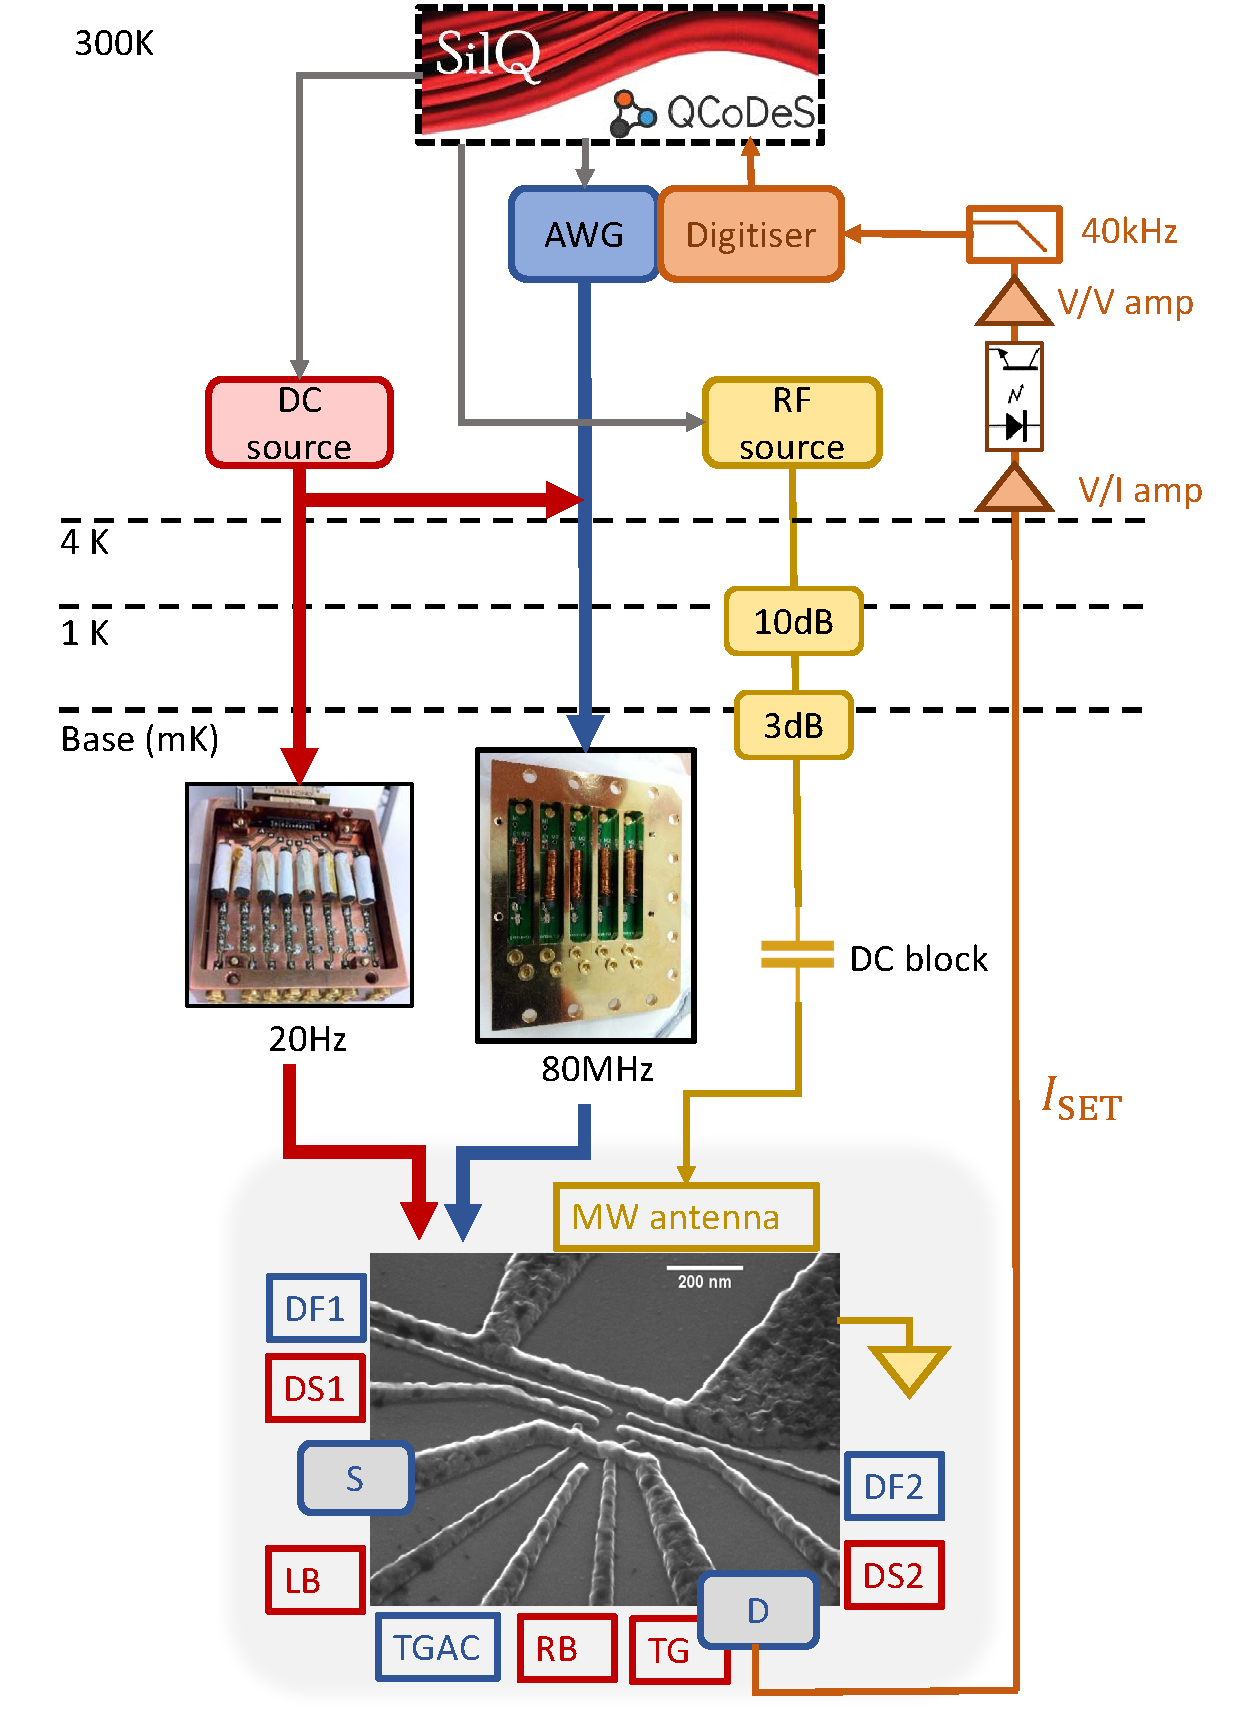
\includegraphics[width=\textwidth]{polished/wiring_queenie.pdf}
	\caption[Electron qubit setup]{\textbf{Electron qubit setup}. Detailed schematics of the experimental setup for the electron qubit.  }
	\label{fig:queenie_setup}
\end{figure}

The qubit has three distinct types of connections to the room temperature world outside of the dilution refridgerator: DC, AC and high frequency ($>80\,$MHz). Each type of connections aims to allow a sufficient amount of power down to the qubit while simultaneously minimizing any thermal noise. Any electrical line emits thermal white noise, called Johnson-Nyquist noise \cite{Johnson, Nyquist} with a power spectral density of $v_n^2=4k_BTR$, where $T$ is the temperature and $R$ the resistance of said line. This noise can be reduced either by attenuation or filtering. We choose our approach according to the line type. 
Figure \ref{fig:queenie_setup} shows the schematic of the line attenuation,  filtering and instrument control used for the electron and nuclear qubit. 

The DC lines require a fixed voltage bias and consist out of the left (LB) and right (RB) SET barrier, the SET top gate (TG), and two donor gates (DS1, DS2). To minimize the Johnson-Nyquist noise as much as possible we filter these lines with a handmade filter box that acts as a low pass filter and attenuates any signal above 20 Hz. It consists out of two passive first-order RC filters in series, with thin-film nichrome resistors of $20\,k\Omega$ and $470\,$nF and $1\,$pF ceramic capacitors, resulting in cut-off frequencies of $20\,$Hz and $8\,$MHz respectively. The lines running from room temperature to the filter box are copper-nickel twisted-pair wires that are thermalized at every temperature stage. 
The AC lines - two more donor gates (DF1, DF2), source (S), drain (D) and the plunger gate (TGAC) - require a fixed voltage bias, but also slow pulsing. Thus we use coppernickel semi-rigid (EZ86) coaxial lines and a filter box with a cut-off frequency of $80\,$MHz instead, consisting of seventh-order integrated LC filters (Mini-Circuits LFCN-80). 
In addition to the passive filters, both filter boxes contain an anti-inductive wound coil with an Eccosorb core in series to reduce high-frequency noise.  Connections from the filter boxes to the enclose are made with MMCX cables. 

The high frequency line needs to transmit pulses of up to $40\,$GHz, thus cannot be filtered. Consequently we use attenuators at different temperature stages to create a good thermal contact between the coaxial signal line of the semi-rigid stainless steel (EZ86) cable and the ground shield which in turn is thermalized to the fridge using copper anchors. These size of the attenuators depends on the required power at the sample and the cooling power at the respective temperature stage. 
We place 10dB of attenuation at 1K and 3dB at mK, which results in a noise temperature of 2K\footnote{300K room temperature noise gets reduced by a factor 10 (10dB) at 4K, leading to 30K additional noise. 34K thermal noise at 4K gets reduced by a factor 2 (3dB) at mK, leading to thermal noise of temperature 17K at the sample}. 
Additionally we add a DC block at mK to remove any DC noise. 

\subsubsection{Instrument control}
All instruments are controlled with our home-built measurement software SilQ \cite{SilQ} which is a python environment built on top of the shared quantum measurement package QCoDes \cite{QCodes}. DC voltages are applied with PXI voltage source card in the measurement computer, directly controlled with SilQ. A TTL pulse generator (SpinCore PulseBlasterESR-PRO) controlled by SilQ is used to trigger all pulses to ensure proper pulse alignment. AC voltages are also supplied by the PXI, however for TGAC, DF1 and DF2 the DC voltage is combined by a resistive combiner with a pulse from the Lecroy ArbStudio arbitrary waveform generator (AWG). ESR pulses are generated by the Agilent E8267D Vector Source. 
The measurement signal of the device consists of the SET current, usually of magnitude of $I\sim 1\,$nA. We amplify the current using a FEMTO DLPCA-200 trans-impedance amplifier set at $10^7\,$V/A. Afterwards the voltage is further amplified by a SIM910 voltage amplifier with a gain of 10 V/V, which also acts as an opto-isolator. This prevents any large ground loop through the fridge. Finally the signal is filtered by a SIM965 analog filter module set to a low-pass fourth order Bessel filter with a cut-off frequency of 40 kHz before it is acquired with the a Keysight Sygnadyne. SilQ controls the data acquisition and transmission from the Sygnadyne temporary storage to the data hard drive.


\subsection{Flip-flop qubit dipole-coupled} \label{sec:setup_dd}

\begin{figure}
	\centering
	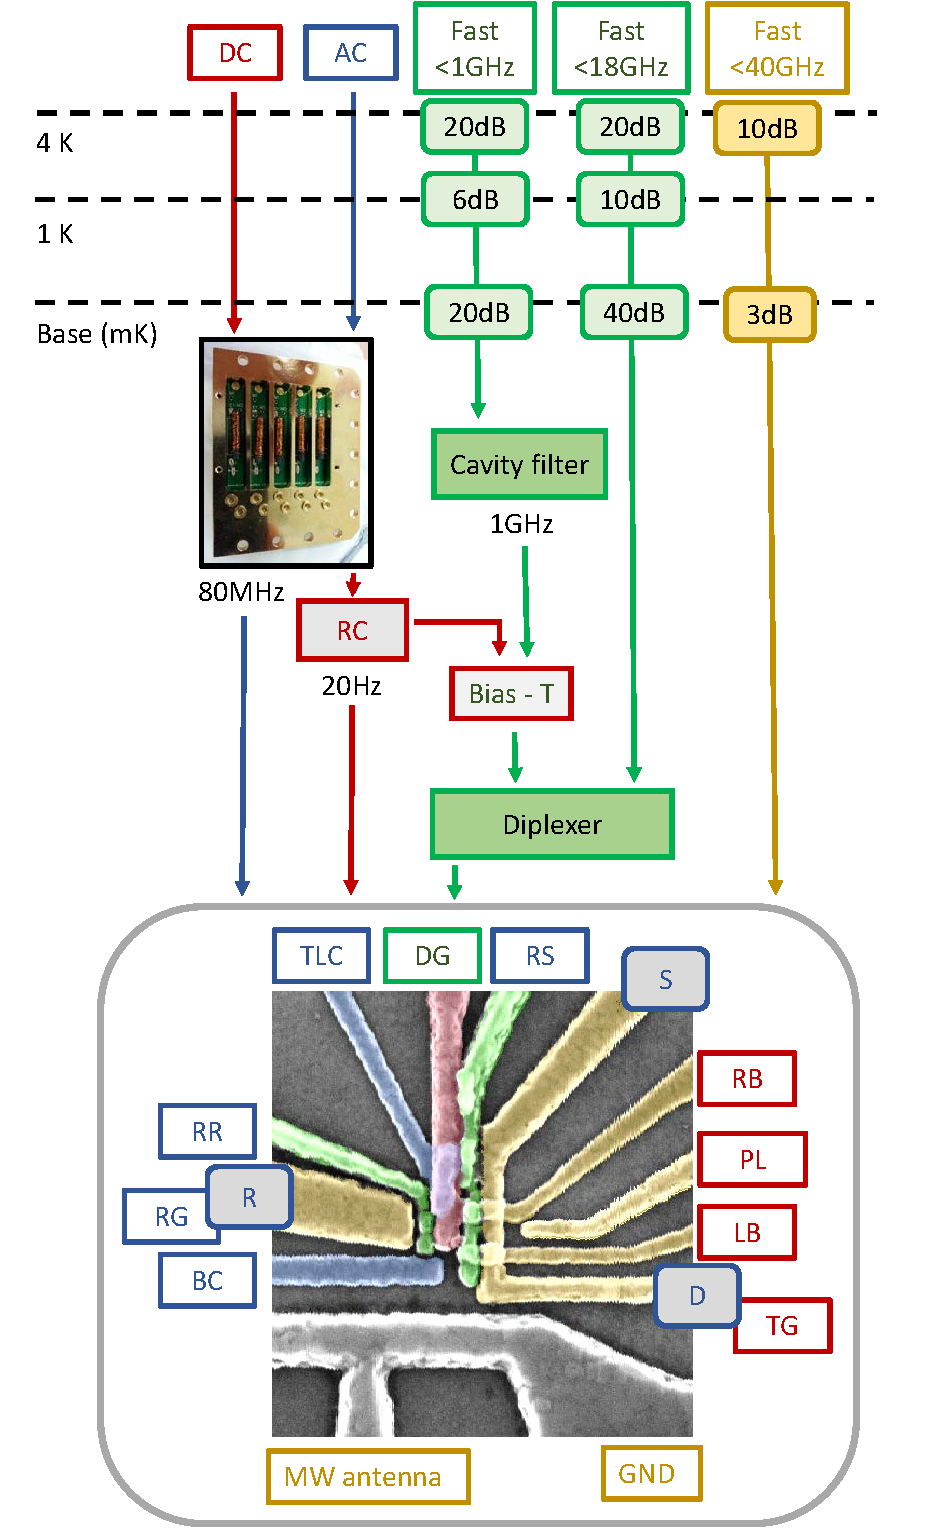
\includegraphics[width=1\textwidth]{polished/wiring_ff.pdf}
	\caption[Flip-flop qubit setup]{\textbf{Flip-flop qubit setup}. Detailed schematics of the experimental setup for the dipole-coupled flip-flop qubit.  }
	\label{fig:dd_setup}
\end{figure}

The setup for the dipole coupled flip-flop qubit (Fig. \ref{fig:dd_setup}) is very similar to the standard electron qubit setup. The qubit has 5 DC lines (RB, LB, TG,  TLC and BC), 7 AC lines (S, D, PL, RS, RR, R and RG) and the high-frequency microwave line. All these lines are wired and operated in the same fashion as for the electron qubit as is the SET readout. The distinct difference to that standard setup is that the donor gate (DG) requires both fast pulsing (GHz) as well as a DC voltage and AC pulsing. To combine these three different frequency lines we use a home-built bias-T and a diplexer XX. 

\begin{figure}
	\centering
	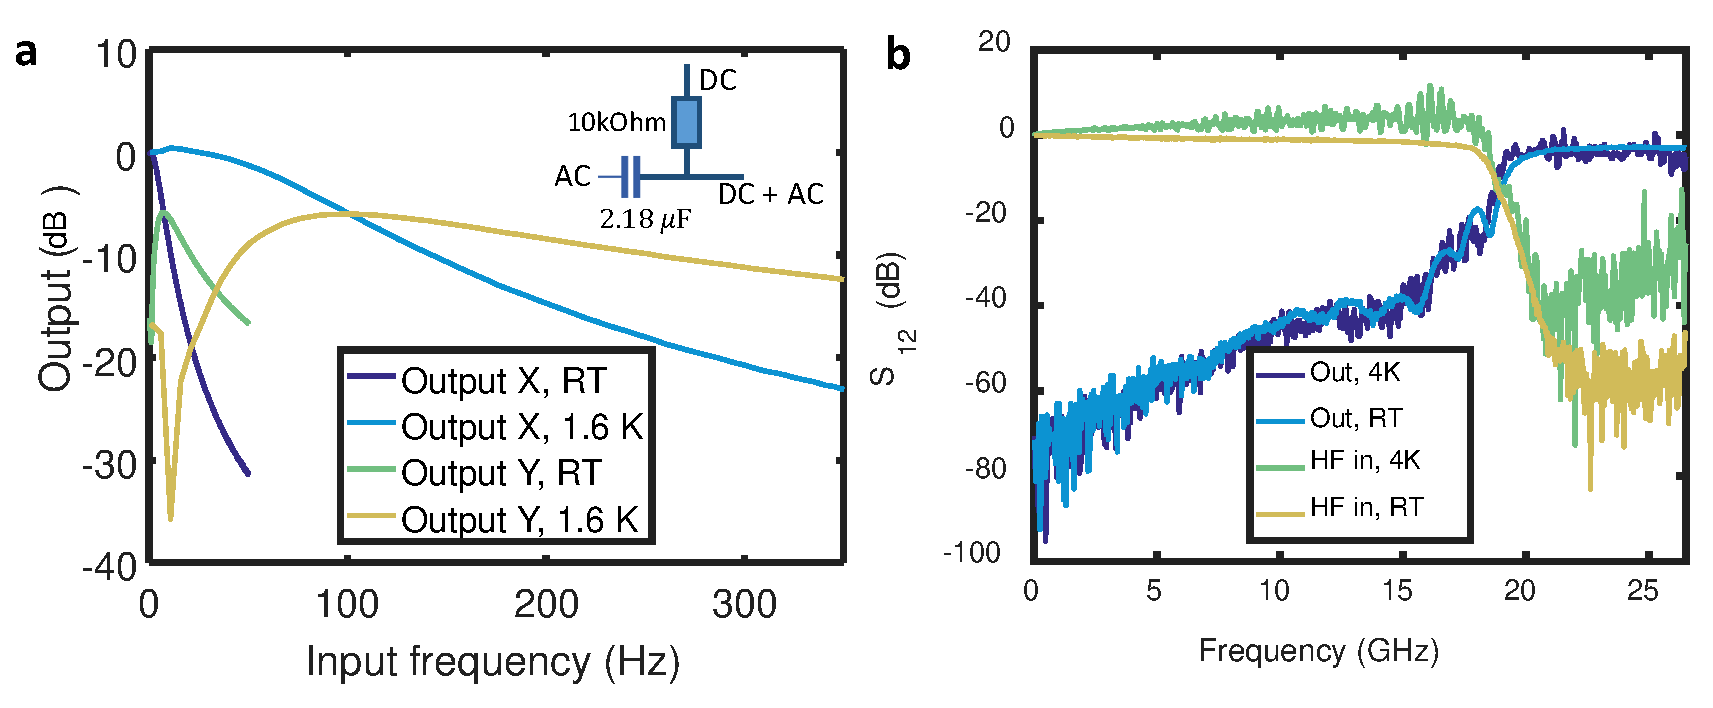
\includegraphics[width=\textwidth]{polished/ff_filtering.pdf}
	\caption[Bias-T and diplexer transmission measurements]{\textbf{Bias-T and diplexer transmission measurements. a} Bias-T transmission from AC to combined port (schematic in top corner) for in-phase(X) and out-of-phase (Y) at 1.6K and room temperature using a lock-in amplifier. The -3dB point shifts from 5Hz at room temperature to 70Hz at 1.6K. \textbf{b} Transmission of the diplexer for input high-frequency (HF) port and the output port at 4K and room temperature using a vector network analyser (VNA). The cut-off frequency is at 18GHz. }
	\label{fig:biast_diplexer}
\end{figure}

The bias-T is comprised of a 10kOhm resistor and a $2.18\,\mu$F ceramic capacitor (see inset figure \ref{fig:biast_diplexer}a) resulting in a cut-off frequency of 5Hz at room temperature which shifts to 70Hz at 1.6K, as measured in figure \ref{fig:biast_diplexer}a. We use this to combine the DC bias from the PXI modules, filtered by the 20Hz filter box, with an attenuated AC pulse from the AWG of up to 1GHz. We choose attenuators of 20dB at 4K, 10dB at 1K and 10dB at mK, giving a noise temperature of 170mK at base
 \footnote{
 %300K room temperature noise gets reduced by a factor 100 (20dB) at 4K, leading to 3K additional noise. 7K thermal noise at 4K gets reduced by a factor 10 (10dB) at 1K, leading to 1.7K additional noise at mK. 1.7K thermal noise at mK gets reduced by a factor 10, leading to a noise temperature of 170mK at the sample. 
 Assuming an applied voltage of 5mV at the sample with a $50\,\Omega$ impedance we create 500nW power dissipation at sample and $5\,\mu$W at mK which can be handled by our dilution refrigerator.}.  

The diplexer passively combines high-frequency and low-frequency pulses by frequency-domain multiplexing with a cut-off at 18GHz, as measured in figure \ref{fig:biast_diplexer}b. We connect the low-frequency port to the output of the bias-T and the high-frequency port to a microwave source with attenuators of 20dB at 4K, 10dB at 1K and 40dB at mK, resulting in a noise temperature of 15mK at base. %\footnote{300K room temperature noise gets reduced by a factor 100 (20dB) at 4K, leading to 3K additional noise. 7K thermal noise at 4K gets reduced by a factor 10 (10dB) at 1K, leading to 0.7K additional noise at mK. 1.7K thermal noise at mK gets reduced by a factor 10 000, leading to a noise temperature of 12mK at the sample. Assuming an applied power of 1pW \cite{Tosi2017} at the sample we create 10nW power dissipation at mK.} 


\subsection{Resonator qubit} \label{sec:setup_res}

\begin{figure}
	\centering
	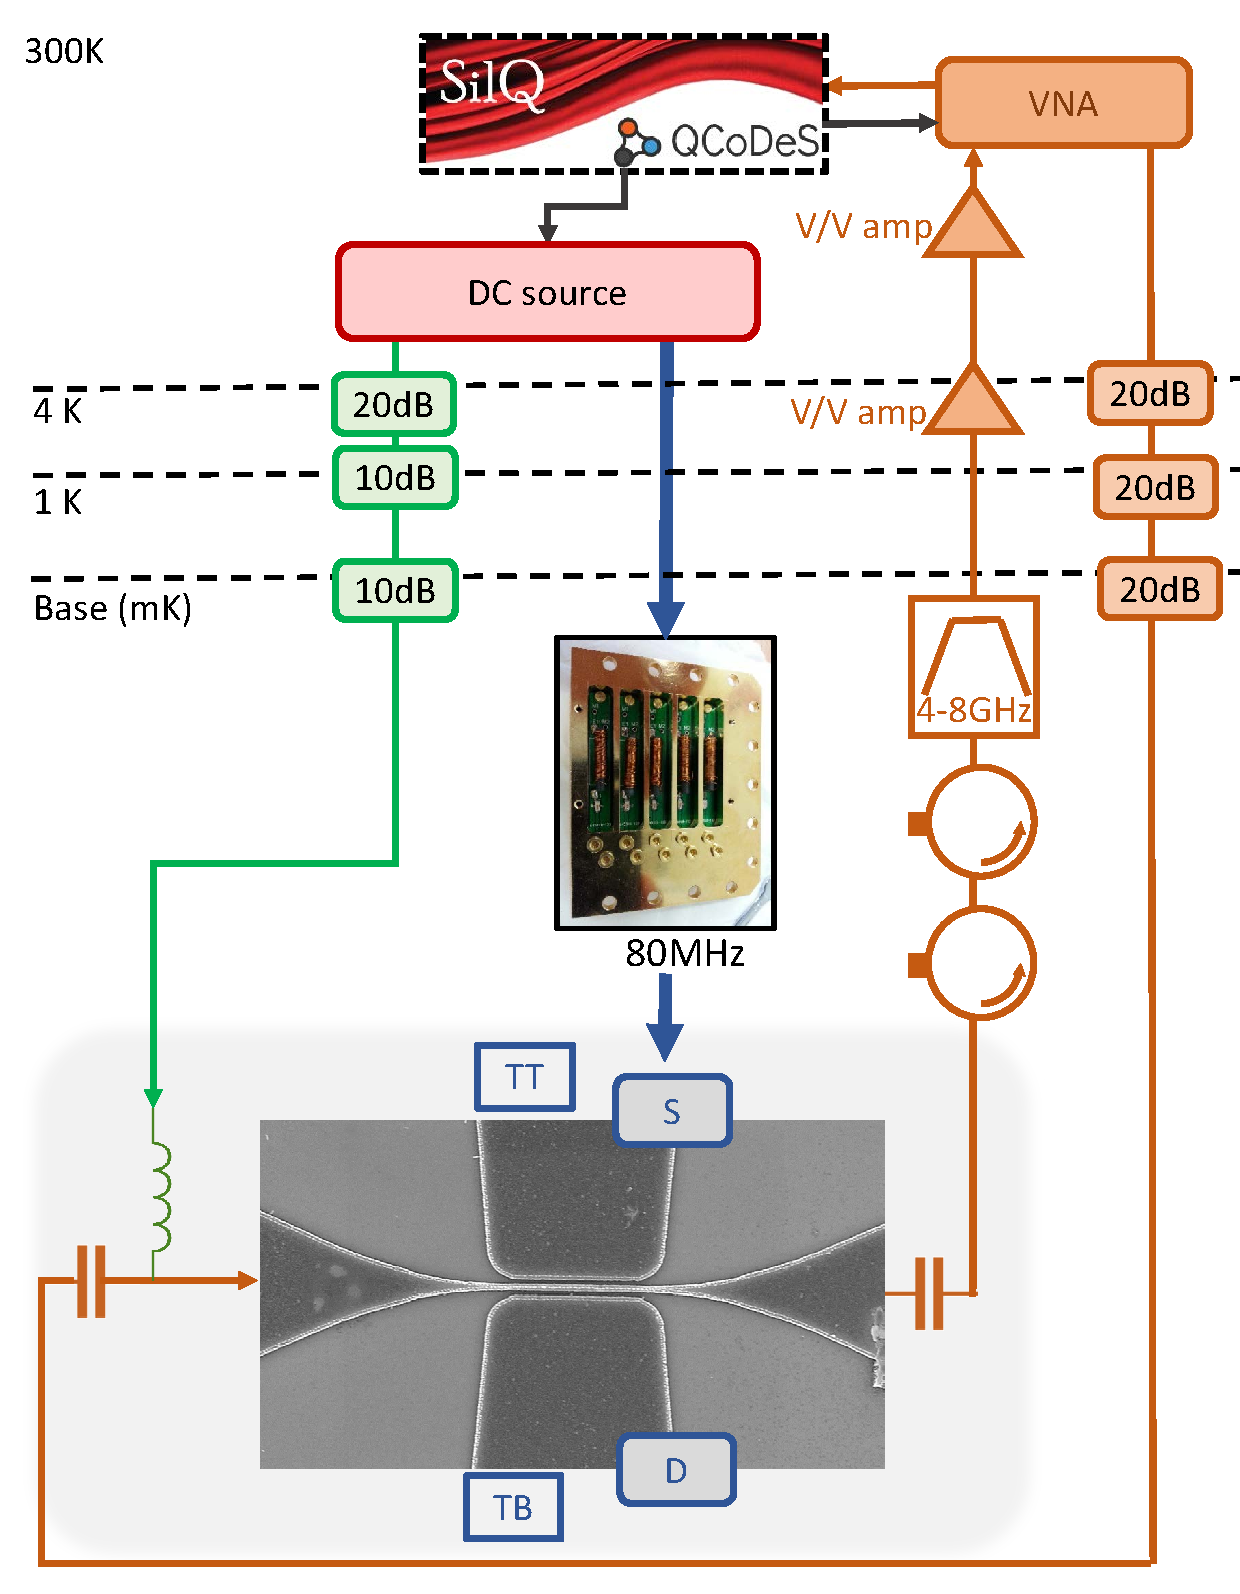
\includegraphics[width=1\textwidth]{polished/wiring_CPWR2.pdf}
	\caption[Flip-flop resonator qubit setup]{\textbf{Flip-flop resonator qubit setup}. Detailed schematics of the experimental setup for the flip-flop qubit coupled to a superconducting resonator.  }
	\label{fig:resonator_setup}
\end{figure}

When coupling our flip-flop qubit to a superconducting resonator, the setup changes significantly from our traditional electron qubit setup. In the simple resonator design the four gates (TT, TB, S, D) are connected via coppernickel semi-rigid (EZ86) coaxial lines to the 80MHz filter box and then at room temperature to the Stanford Research Systems (SRS) SIM928 Isolated Voltage Source modules in a SIM900 mainframe. These lines are thermalized at every temperature stage. 
The central conductor is biased through an on-chip inductor by the SIM module with attenuation of 20dB at 4K, 10dB at 1K and 10dB at mK, same as for the AC line of the dipole-coupled flip-flop qubit donor gate. 

Readout is performed through the resonator. We operate in transmission mode. The input signal is generated by the VNA and attenuated by 20dB at each temperature stage (noise temperature of 120mK .
%\footnote{300K room temperature noise gets reduced by a factor 100 (20dB) at 4K, leading to 3K additional noise. 7K thermal noise at 4K gets reduced by a factor 100 (20dB) again at 1K, leading to 70mK additional noise at 1.K. 1.07K thermal noise at 1K gets reduced by a factor 100, leading to a noise temperature of 120mK at the sample.}). 
The output signal is routed through two isolators to reduce any thermal noise coming down the line and a 4-8 GHz bandpass filter to reduce any noise before amplification. The signal then passes a cryogenic amplifier with dB gain and a room temperature amplifier with dB gain before entering the VNA. SilQ controls the SIM modules and the VNA. 

\subsubsection{Advanced resonator design}

\begin{figure}
	\centering
	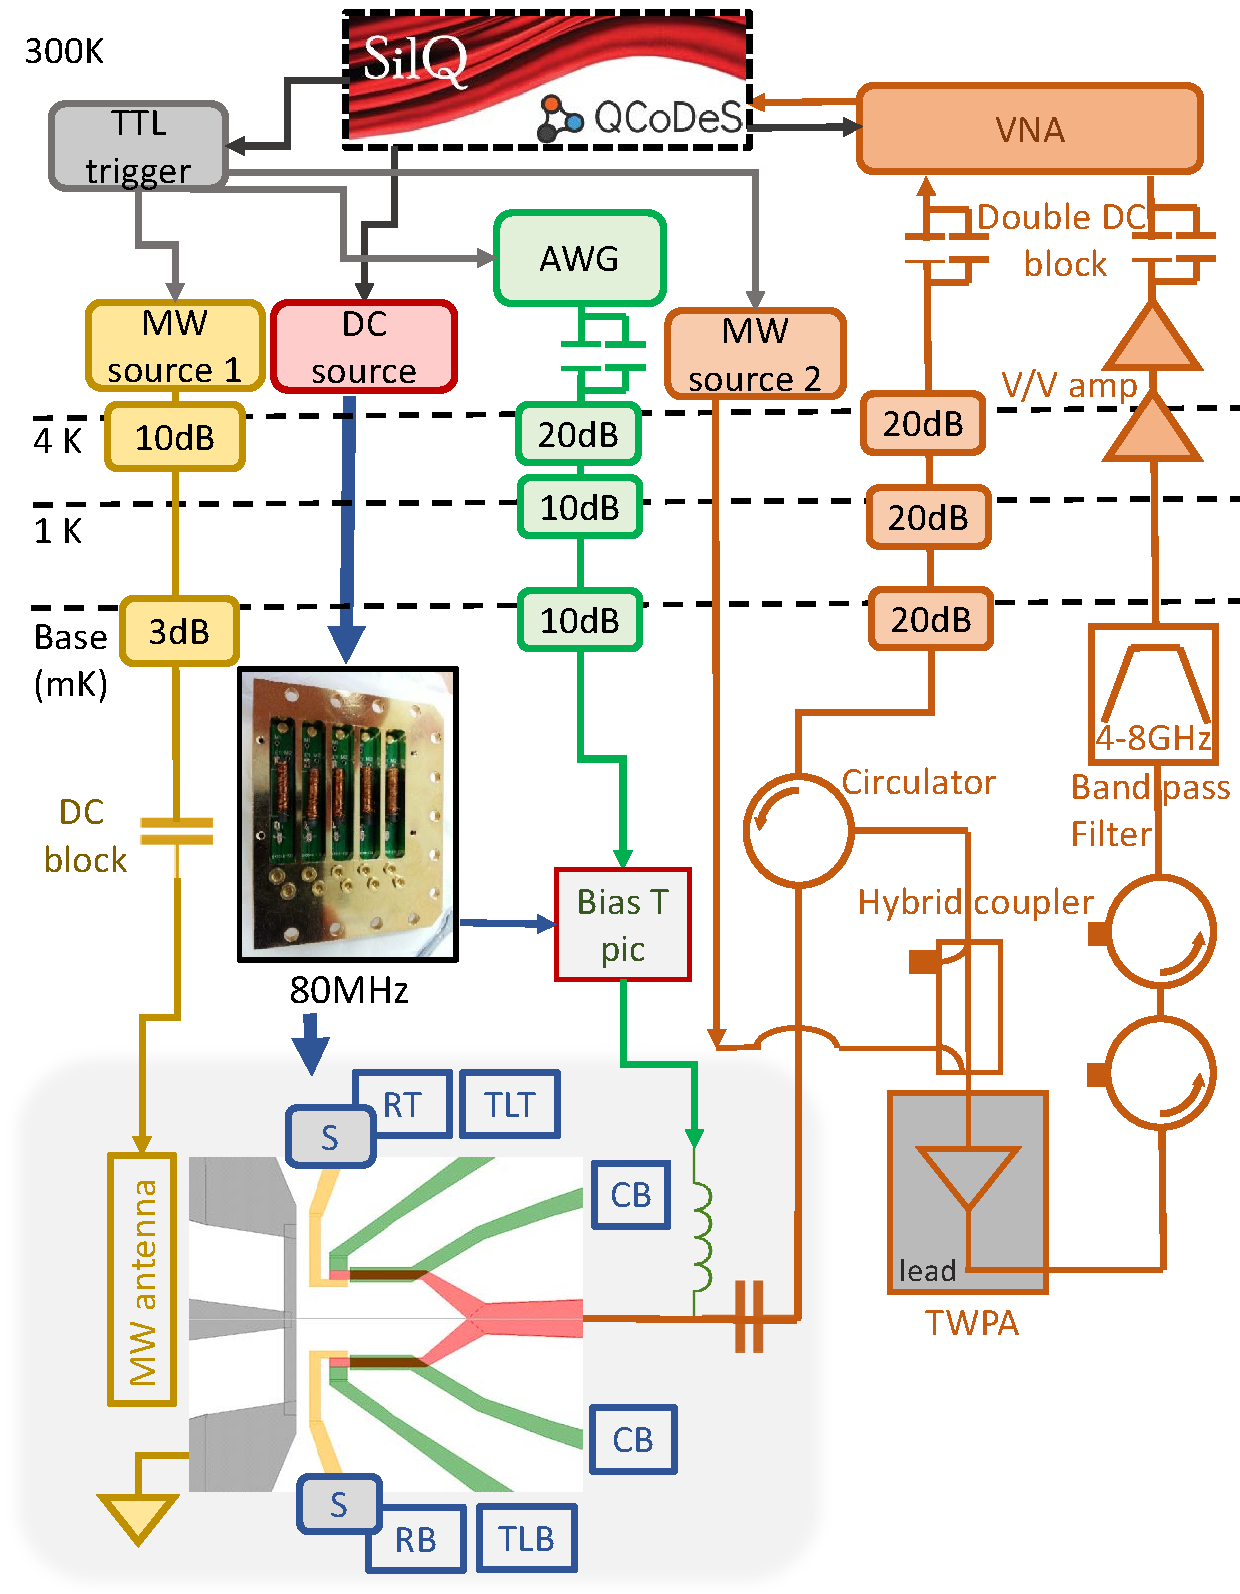
\includegraphics[width=1\textwidth]{polished/wiring_CPWR_VS.pdf}
	\caption[Advanced flip-flop resonator qubit setup]{\textbf{Advanced flip-flop resonator qubit setup}. Detailed schematics of the experimental setup for the flip-flop qubit coupled to a superconducting resonator with the advanced design.  }
	\label{fig:resonator_setup_new}
\end{figure}

The setup for the advanced resonator design is more complex as we now not only have several additional gates and a microwave antenna but also are operating the resonator in reflection. It is basically a hybrid between the simple resonator design and the dipole design with some additional components for good reflective resonator operation.

The microwave antenna and the AC gates (S, RT, TLT and CB) are connected as for the dipole-coupled qubit in section \ref{sec:setup_dd}, with difference that each gate has its own on-chip inductor to reduce coupling into the resonator.  
The central conductor is biased through the on-chip inductor as for the simple resonator design. However, we prefer to use a bias-T as for the dipole design to better filter the line. 

The resonator is connected on one port only where the signal is send in, reflected and then measured. 
The signal is generated by the VNA, attenuated by 20dB on each temperature stage, passes through a circulator and reaches the resonator. Then the signal is reflected, travels up the same line, enters the circulator where it is separated from the input signal. It is then fed into a hybrid coupler where the signal is combined with a pump tone from a second microwave source of a frequency and power calibrated to the signal. This tone is required at the next stage, the Josephson travelling-wave parametric amplifier (TWPA), which amplifies the signal up to 20dB over a 3GHz bandwidth \cite{Macklin2015}. Following is the same readout setup as for the simple design. We add double-DC blocks on all high-frequency lines to reduce DC current noise. 




 
% Chapter Template

\chapter{Flip-flop qubit measurements} % Main chapter title

\label{Chapter7} % Change X to a consecutive number; for referencing this chapter elsewhere, use \ref{ChapterX}

\HRule
\vspace{0.5cm} \hspace{2cm}
\small
\hangindent=4cm
\\
        ``\emph{hopefully sth here...}"
\\ \\
\hangindent=4cm
\begin{flushright}
--? \\
\end{flushright}

\vspace{0.5cm}

\noindent \HRule
\clearpage

\section{Proof of principle Flip-flop measurement} \label{sec:ff_resonance}

\begin{figure}
	\centering
	\includegraphics[width=0.9\textwidth]{polished/ff_spectrum.pdf}
	\caption[Flip-flop qubit resonance]{\textbf{Flip-flop qubit resonance. a}}
	\label{fig:ff_spectrum}
\end{figure}

\section{Dipole-dipole coupling devices} \label{sec:dd_meas}

\begin{figure}
	\centering
	\includegraphics[width=\textwidth]{polished/turnon_pinchoff.pdf}
	\caption[Flip-flop qubit turn on and pinch-off]{\textbf{Flip-flop qubit turn on and pinch-off. a}}
	\label{fig:turnon_pinchoff}
\end{figure}

\begin{figure}
	\centering
	\includegraphics[width=\textwidth]{polished/CoulombOscillations.pdf}
	\caption[Flip-flop qubit Coulomb oscillations and diamonds]{\textbf{Flip-flop qubit Coulomb oscillations and Coulomb diamonds. a}}
	\label{fig:coulomb_oscillations}
\end{figure}

\begin{figure}
	\centering
	\includegraphics[width=\textwidth]{polished/stability_diagram_ff.pdf}
	\caption[Flip-flop qubit charge stability diagram]{\textbf{Flip-flop qubit charge stability diagram. a}}
	\label{fig:coulomb_oscillations}
\end{figure}


\section{CPWR devices} \label{sec:cpwr_meas}

\subsection{Resonator characterization}

\begin{figure}
	\centering
	\includegraphics[width=\textwidth]{polished/resonance_fit.pdf}
	\caption[Flip-flop qubit turn on and pinch-off]{\textbf{Flip-flop qubit turn on and pinch-off. a}}
	\label{fig:resonance_fit}
\end{figure}

\begin{figure}
	\centering
	\includegraphics[width=\textwidth]{polished/cpwr_temp.pdf}
	\caption[Flip-flop qubit turn on and pinch-off]{\textbf{Flip-flop qubit turn on and pinch-off. a}}
	\label{fig:cpwr_temp}
\end{figure}

\begin{figure}
	\centering
	\includegraphics[width=\textwidth]{polished/cpwr_bfield.pdf}
	\caption[Flip-flop qubit turn on and pinch-off]{\textbf{Flip-flop qubit turn on and pinch-off. a}}
	\label{fig:cpwr_bfield}
\end{figure}



\subsection{2DEG influence}

\subsubsection{Low Q}

\begin{figure}
	\centering
	\includegraphics[width=\textwidth]{polished/ResonanceTurnon.pdf}
	\caption[Flip-flop qubit turn on and pinch-off]{\textbf{Flip-flop qubit turn on and pinch-off. a}}
	\label{fig:lowq_turnon}
\end{figure}

\begin{figure}
	\centering
	\includegraphics[width=\textwidth]{polished/Resonance2DEG.pdf}
	\caption[Flip-flop qubit turn on and pinch-off]{\textbf{Flip-flop qubit turn on and pinch-off. a}}
	\label{fig:lowq_2deg}
\end{figure}

\subsubsection{High Q}

\begin{figure}
	\centering
	\includegraphics[width=\textwidth]{polished/highq_turnon.pdf}
	\caption[Flip-flop qubit turn on and pinch-off]{\textbf{Flip-flop qubit turn on and pinch-off. a}}
	\label{fig:highq_turnon}
\end{figure}

\begin{figure}
	\centering
	\includegraphics[width=0.6\textwidth]{polished/2deg_mag.png}
	\caption[Flip-flop qubit turn on and pinch-off]{\textbf{Flip-flop qubit turn on and pinch-off. a}}
	\label{fig:highq_2deg}
\end{figure}

\subsection{Power influence}


\begin{figure}
	\centering
	\includegraphics[width=0.6\textwidth]{polished/power_mag.png}
	\caption[Flip-flop qubit turn on and pinch-off]{\textbf{Flip-flop qubit turn on and pinch-off. a}}
	\label{fig:res_power}
\end{figure}


\subsection{Charge qubit} \label{sec:res_chargequbit}
 
% Chapter Template

\chapter{Low magnetic field effects in Si:P qubits} % Main chapter title

\label{Chapter6} 


\HRule
\vspace{0.5cm} \hspace{2cm}
\small
\hangindent=4cm
\\
        ``\emph{Improving and understanding the performance of our qubit}"
\\ \\
\hangindent=4cm
\begin{flushright}
--? \\
\end{flushright}

\vspace{0.5cm}

\noindent \HRule
\clearpage



\section{\label{sec:introduction}Introduction}

The electron spin-lattice relaxation time $T_1$ in donors in silicon is of great interest. Not only gives it insight into the fundamental physics of the system but also is extremely relevant for donor spin qubits which have proven to be excellent candidates for quantum computation \cite{Muhonen2014, Muhonen2015}. Indeed the qubit coherence times of up to $T_2=1\,$s approach the limit set by the relaxation time \cite{Kalra2016}. However, few experiments have been performed to learn more about the mechanisms limiting $T_1$. 

Generally, relaxation happens due to fluctuations in the transverse elements of the Hamiltonian at the Larmor frequency of the spin states. This requires the spin to be coupled to a phonon reservoir.
As silicon is not a piezoelectric material this coupling is only achieved by the deformation potential. Phonons, in form of acoustic waves, deform the lattice while travelling through the crystal. This breaks crystal cubic symmetry which in turn lifts the degeneracy of the six conduction band minima, called valleys. The magnitude of this energy shift is defined by the deformation potential. The relative valley population changes, causing a shift in the g-factor. This shift oscillates with the phonon frequency and relaxes the spin \cite{Hasegawa1960}. Furthermore, local strain couples the $\Gamma$ and $\Delta$ energy bands in one valley, effectively changing the g factor locally, thus also relaxing the spin in the same fashion \cite{Roth1960}. 
This spin-lattice relaxation is described by 
\begin{eqnarray}\label{eq:fullT1}
T_1^{-1} & = & \frac{1}{90\pi}\left(\frac{g_{||}-g_\perp}{g_0}\right)\left(\frac{\Xi_u}{E_{12}}\right)^2\\
& &\left(\frac{1}{\rho \bar{v}_t^5}+\frac{2}{3\rho\bar{v}_l^5}\right)\left(\frac{g_0\mu_0B}{\hbar}\right)^4f(\theta)\cdot k_{\rm B} T
\end{eqnarray}
in the high temperature limit where $\frac{g_{||}-g_\perp}{g_0}$ is the anisotropy in the g-factor, $\Xi_u$ is the deformation potential, $E_{12}$ is the valley orbit splitting between the ground and first excited state, $v_l, v_t$ are the sounds velocities in silicon, $\rho$ is the density of silicon and $f(\theta)$ is an angular factor with regard of the external magnetic field $B_0$ and the crystal axis \cite{Wilson1961}.
At low temperatures ($k_{\rm B}\ll E_z=g_0\mu_0 B$) only spontaneous phonon emission is possible so that $T_1\sim B^5$ is expected \cite{Morello2010, Zwanenburg2013}. 

Previously the dependence of $T_1$ on external magnetic field at low temperatures of donors in silicon has been measured by Morello \textit{et. al.} \cite{Morello2010} on two single phosphorus donors in a CMOS style device and Watson \textit{et. al} \cite{Watson2015} on a single phosphorus donor in a STM hydrogen lithography device. While two of these three measurements conform with each other and follow the expected $T_1\sim B^5$, one measurement by Morello \textit{et. al.} shows a strong deviation. Not only is the magnitude of the $B^5$ relaxation one order of magnitude different but also deviates the measurement from $T_1\sim B^5$ to $T_1\sim B$ at low magnetic fields $B<2\,$T.  

In this paper we present detailed measurements of the relaxation with magnetic field in both enriched silicon $^{28}$Si and natural silicon. We find large deviations in behaviour between different samples which implies a strong dependence of the relaxation on the donor environment. We see a clear $T_1\sim B$ at low magnetic fields for most samples. This dependence seems to be caused by Evanescent wave Johnson noise (EWJN). The magnitude of the $B^5$ relaxation varies by two orders of magnitude between the measured samples. The cause for this effect remains uncertain, though it could be caused by a different concentration of Si29 nuclei or strain variations. Further investigation is necessary. 

Moreover, as the relaxation time approaches multiple seconds, we observe effects of the electro-statical environment on the relaxation. Thus, we study the relaxation with both donor confinement depth (plunge voltage) and the electron number on a nearby single electron transistor (SET). We observe direct tunnelling into the nearby SET electron reservoir reducing the relaxation time for shallow plunging. Once this first-order process is suppressed, second-order tunnelling limits the relaxation time until all tunnelling processes are suppressed at deep plunge voltages $V_p\gg E_z$.

%This study revealed three different effects that influence the relaxation time in this system:  Firstly, we observe an effect that leads to a dominant . 
% EWJN relaxes the donor electron by stimulated emission into the enhanced density of states of the electromagnetic waves decaying from the Aluminium structures on top of the donor.
% Secondly, strain strongly suppresses the phonon relaxation. Lastly, co tunnelling decreases the $T_1$ if the donor is not plunged deep enough below the Fermi level.
 % The $\ket{\uparrow}$ electron escapes from the donor through a virtual co-tunnelling process into free states of the reservoir of the SET island and is replaces by $\ket{\downarrow}$. The tunnel rate strongly depends on the depth of the donor level beneath the Fermi level. Thus it can be mitigated by pulsing deeply below the Fermi level during operation.

The remainder of this paper will elaborate on these findings and is organised as follows. Section \ref{sec:background} presents our physical system and the experimental set up as well as the measurement techniques used to acquire the data. Then section \ref{sec:extB} shows the results of the magnetic field dependence measurements where we both analyse the low magnetic field behaviour in section \ref{sec:ewjn} and the high magnetic field behaviour in section \ref{sec:strain}. Lastly, section \ref{sec:cotunnelling} presents the electrostatic environment measurements. Finally, section \ref{sec:conclusion} discusses the results, open questions and possible future measurements. 


\section{\label{sec:background} The qubit system and measurement methods}

\begin{figure}
\centering
\includegraphics[width=\columnwidth]{figures/fig1.pdf}
\caption{
(a) Schematic of a phosphorus donor implanted in enriched $^{28}$Si with a scanning electron micrograph of an identical device to the one measured. Four gates control the donor potential while a single electron transistor (SET) detects electron tunnel events in its environment to determine the qubit state. A broadband microwave antenna provides an electromagnetic drive for both the electron and the nucleus. b) Energy diagram of the electron-nuclear spin system, with ESR and NMR transitions indicated. (c) Schematic of the two regimes the donor qubit is operated in for the relaxation measurements: 1. Readout regime, where the donor is tuned such that the Fermi level of the SET reservoir lies below $\ket{\uparrow}$ and the electron can tunnel out, producing a current spike, while $\ket{\downarrow}$ lies above and stays confined, keeping the current low. 2. Operating regime, where both spin states are well confined below the Fermi level.
}
\label{fig:device}
\end{figure}

Our qubit is a single electron spin confined by a phosphorus $^{31}$P donor implanted in enriched $^{28}$Si as shown in the schematic in figure \ref{fig:device} (a). An external magnetic field is applied to separate the spin states into a well defined two level system. This leads to a two-qubit system: The donor electron with $S=1/2$ and basis states $\ket{\uparrow},\ket{\downarrow}$ and the $^{31}$P nucleus with $I=1/2$ and basis states $\ket{\Uparrow},\ket{\Downarrow}$. The energy levels of this system are displayed in figure \ref{fig:device} (b). A scanning electron micrograph of the device is shown in figure \ref{fig:device} (a).  Aluminium gates on top of the donor control the electrostatic environment and are used to apply DC pulses while a broadband microwave antenna is used for microwave and radio frequency pulses, allowing for full control over the qubit states. A nearby SET with an electron reservoir of an electron temperature of $T\approx 100\,$mK acts as a readout mechanism for the electron spin state. Therefore, we tune the electrochemical potential of the SET $\mu_{\rm SET}$ and the donor $\mu_d$ such that the donor electron tunnels to the SET reservoir if in state $\ket{\uparrow}$, causing a SET current spike, but stays confined if $\ket{\downarrow}$. This tuning configuration we call the "readout regime", illustrated in figure \ref{fig:device} (c). 
This paper focusses on the electron qubit only. For the experiments in this paper the qubit is operated in two regimes: Firstly, the readout regime. Secondly, the operating regime, where the donor is tuned such that both electron spin states are well confined below the Fermi level of the SET, as illustrated in figure \ref{fig:device} (c). 


\subsection{\label{sec:Measurementprocedures} Measurement procedures}

\begin{figure}
\centering
\includegraphics[width=0.7\columnwidth]{figures/fig2.pdf}
\caption{
(a) Schematic of the pulse sequence used in the experiments. The solid line represents the position of the donor energy levels with respect to the Fermi level achieved by the combined voltages of the donor gates. For fields $B_0\leq1.5\,$T, $\ket{\downarrow}$ is initialized and then inverted with an ESR $\pi$-pulse to achieve higher contrast while for $B>1.5\,$T a random load is performed. (b) Example of a $T_1$ measurement at $B=1.5\,$T. For each plunge duration $30$ single shots are taken and averaged to a single point (small black dots). Then the whole measurement is repeated several times and averaged (blue dots) to account for drifts and fluctuations. This uncertainty is expressed through the standard deviation error bars. The relaxation time is extracted by a least-square fit to $T_1=3.7\pm0.4\,$s.
}
\label{fig:t1example}
\end{figure}

To determine the relaxation time $T_1$ of the electron we repeatedly measure the $\ket{\uparrow}$ proportion after a period of time $\tau$ has elapsed while the donor is in the operating regime.  The applied pulse sequence is illustrated in figure \ref{fig:t1example} (a). First, we initialize the electron in $\ket{\downarrow}$ for external magnetic fields of $B_0<1.5$T. Therefore we tune to the readout regime and wait for roughly the tunnel time ($20\,$ms) so that $\ket{\uparrow}$ tunnels into the reservoir and is replaced by $\ket{\downarrow}$. If a high precision is required to increase the measurement contrast, we apply a technique called Bayesian update. A feedback loop is applied that self-corrects for wrongly loaded $\ket{\uparrow}$ and can achieve initialization fidelities of over $99\%$ \citep{Johnson2018}. After $\ket{\downarrow}$ initialization, $\ket{\downarrow}$ is inverted to $\ket{\uparrow}$ by applying an electron spin resonance (ESR) $\pi$-pulse. This concludes the initialization phase. Next, the donor remains for time $\tau$ in the operating regime at plunge depth $V_{p}$. Lastly, a single shot readout is performed in the readout regime. We repeat this sequence $30$ times to acquire one data point of corresponding $\tau$ and then repeat the full measurement multiple times to account for drifts and fluctuations in the electrostatic environment. Figure \ref{fig:t1example} (b) shows an example measurement of the relaxation time at $B_0=1.5$T. The $T_1$ time is extracted by performing a least-square fit. For $B_0>1.5\,$T a random load is performed by simply emptying and reloading an electron, thus preparing either $\ket{\uparrow}$ or $\ket{\downarrow}$ randomly. The remainder of the pulse sequence is the same. The plunge voltage $V_p$ is created by biasing two of the donor gates and the SET top gate simultaneously, changing the electrochemical potential of the donor $\mu_d$ electron with respect to the Fermi level of the SET island. Unless otherwise stated, these pulses are compensated which means that bias of the donor and SET top gate is performed with such a ratio that the SET Fermi level is kept constant while moving the donor. 


\section{Relaxation time dependence on external magnetic field} \label{sec:extB}

\begin{figure}
\centering
\includegraphics[width=\columnwidth]{figures/fig3.pdf}
\caption{(a) Measurements of the dependence of electron spin-lattice relaxation time $T_1$ on the external magnetic field $B_0$ from different samples. Device 2010A and 2010B are taken from \cite{Morello2010} and are natural silicon, same as device 2011A (squares). Device 2017A and 2018A have been measured on Si$^{28}$, as have devices 2013A and 2013B (dots). For device 2010A, B, 2017A and 2018A curves of form $A_1B_0+A_5B_0^5$ have been fitted. For comparison a measurement of a bulk Si:P crystal at $T<5\,$K is shown (Morton). (b) Fit results of the different samples. 
}
\label{fig:magnetic field dependence}
\end{figure}


In this section we are analysing the dependence of the relaxation time on the strength of the external magnetic field $B_0$. Figure \ref{fig:magnetic field dependence} (a) shows sets of relaxation rates with magnetic field for seven donor qubits with almost identical device layout: devices 2010A and 2010B which are  natural silicon samples, taken from \cite{Morello2010},
device 2011A, also on natural silicon and devices 2013A, 2013B, 2017A, 2018A which are enriched Si$^{28}$ samples. We fit devices 2010A, 2010B, 2017A and 2018A with a polynomial of type $A_0+A_1B_z+A_5B_z^5$ with the results displayed in the table of figure \ref{fig:magnetic field dependence}.  The magnitude of the $B^5$ dependence at high magnetic fields varies significantly between the different devices. This will be explored in section \ref{sec:phonon}.
Furthermore, all fitted devices show a deviation from the expected $T_1\sim B^5$ at magnetic fields below $B_0\approx3\,$T, except for device 2010B. Devices 2010A and 2017A behave as $T_1\sim B_0^1$ while 2018A behaves as $T_1\sim \rm{const.}$. The following section explores an explanation for the $T_1\sim B_0^1$ behaviour.

\subsection{\label{sec:ewjn}Evanescent wave Johnson noise}

\begin{figure}
\centering
\includegraphics[width=\columnwidth]{figures/fig4.pdf}
\caption{
(a)Schematic of the origin of EWJN in our qubit devices. (b) Scanning electron micrograph of a Hall bar structure with feature size of $30\,$nm. (c) Table of conductance values of Aluminium, measured with  Hall bar structures as in (b), for different feature sizes and evaporation techniques. Aluminium thickness is 50nm. Room temperature bulk value for comparison \cite{Serway1998}. (d) Geometry assumption for theoretical EWJN calculations where the cylinder represents the metal gate on top of the qubit (small yellow circle) with diameter $a$ and distance $d$. (e) Table of relaxation rates predicted by the EWJN theory and measured value at $B_0=1.5\,$T. 
}
\label{fig:ewjn}
\end{figure}

Our qubits are in the vicinity of metal electrodes that contain mobile charges and spins. The thermal and quantum motion of these creates random electromagnetic fields that decohere and relax the qubit. This we know as Johnson noise \cite{Johnson1928, Nyquist1928, Callen1951}. It leaks out of the metal into the insulator in form of evanescent waves when the photons are reflected on the metal-insulator interface as depicted in figure \ref{fig:ewjn}. Thus there is strong Johnson noise near the metallic surface which is called evanescent wave Johnson noise (EWJN) \cite{Henkel1999, Poudel2013, Premakumar2017}. At low temperatures this can lead to relaxation as the evanescent waves create many available photon states which enhances spontaneous emission for the donor electron. For this type of magnetic noise that couples directly to the electron spin, we can write for $k_BT\ll g_0\mu_B B_0$ the relaxation rate as

\begin{equation}
T_1^{-1}=\frac{1}{\mathcal{L}}\frac{\mu_B^2\sigma\omega_0}{\hbar c^2}
\end{equation}

where $\mathcal{L}$ is a geometric factor that depends on the geometry of the device, $\sigma$ is the conductivity of the metal structures, $\omega_0$ is the Larmor frequency of the qubit which depends on the magnetic field $\omega_0=\frac{g_0\mu_B B_0}{\hbar}$. $g_0$ is the electron g-factor, $\hbar$ the reduced Plank constant, $c$ the speed of light in vacuum and $\mu_B$ the Bohr magneton. Thus the relaxation follows $T_1^{-1}\sim B_0$. This theory anticipates a local response. Consequently the skin depth $\delta=1/\sqrt{\mu_0\mu_R\sigma\omega_0/2}$ has to be large compared with the dimensions of the metallic elements of the device and the distance of the qubit from those objects. Furthermore, the conduction in the electrodes has to be in the diffusive regime where the mean free path $l_F=v_F\frac{m_e}{ne^2}\sigma$ ($v_F$ is the electron Fermi velocity, $m_e$ the electron mass, and $n$ the electron density) is much shorter than the device dimensions.  

As the conductance of the aluminium structures directly relates to both the validity of the model through the characteristic length scales and the resulting magnitude of the relaxation, we carefully measure it with 4-point measurements on Hall bar structures with feature sizes varying from $300\,$nm to $30\,$nm for both thermal and electron beam physical vapour deposition (EBPVD). Figure \ref{fig:ewjn} (b) shows a scanning electron micrograph of a $30\,$nm Hall bar device while table \ref{fig:ewjn} (c) shows the resulting conductance values for all measured structures. 
We find that the conductivity drops with reduced feature size but only up to a factor of 2 which is conclusive with our feature size of approximately $20\,$nm.  We choose the $30\,$nm thermal measurement $\sigma=1.6\cdot 10^7\,$S/m for further calculations as this resembles most closely the qubit device measured in this paper. This results in a skin depth of $\delta=752\,$nm and mean free path of $l_F=19\,$nm. Thus, while the skin depth is sufficiently large, the mean free path is comparable with our feature size of around 30nm. This means that we are on the brink between the ballistic and diffusive regime which might reduce the EWJN.

We calculated the geometric dependence according to our device geometry by assuming a conducting cylinder of diameter $a$ and distance $d$ from the qubit as shown in figure \ref{fig:ewjn} (d). In our case $d$ and $a$ are of similar magnitude. Thus we employ an interpolation between the qubit seeing a half-space sphere ($d\rightarrow 0$) and the qubit being far away ($d\gg a$) which predicts the relaxation rate to 
\begin{subequations}
\begin{equation}
T_{1,x}^{-1}=\frac{\mu_B^2\sigma\omega_0}{\hbar c^2d}\frac{\frac{75\pi^2}{1024}\frac{a^4}{d^4}\frac{3\pi}{4}}{\frac{75\pi^2}{1024}\frac{a^4}{d^4}+\frac{3\pi}{4}}
\end{equation}
\begin{equation}
T_{1,y}^{-1}=\frac{\mu_B^2\sigma\omega_0}{\hbar c^2d}\frac{\frac{273\pi^2}{1024}\frac{a^4}{d^4}\frac{3\pi}{4}}{\frac{273\pi^2}{1024}\frac{a^4}{d^4}+\frac{3\pi}{4}}
\end{equation}
\begin{equation}
T_{1,z}^{-1}=\frac{\mu_B^2\sigma\omega_0}{\hbar c^2d}\frac{\frac{147\pi^2}{512}\frac{a^4}{d^4}\frac{\pi}{2}}{\frac{147\pi^2}{512}\frac{a^4}{d^4}+\frac{\pi}{2}}
\end{equation}
\end{subequations}

With our experimental parameters, EWJN predicts relaxation rates of $T_1\approx5\,\rm{s}^{-1}$ as shown in table \ref{fig:ewjn} (e). We find our theory to agree well with our measurement of device 2013A while it overestimates the relaxation rate by around one order of magnitude for device 2017A. We have to keep in mind though that the donor depth is uncertain within $\pm10\,$nm due to the implantation process \cite{VanDonkelaar2015}, as well as the exact donor position with regard to the metal gates. This can account for variations between different devices, even though the same metal gate structure was used. Nevertheless a donor depth much beyond $20-,$nm seems unreasonable, given that we are able to easily readout the donor with our SET. Thus the theory indeed seems to overstate the EWJN relaxation. This is quite puzzling. One explanation could be that ballistic effects reduce the EWJN. Additionally, the interpolation formula seems to be favouring the near-limit, thus potentially overestimating the relaxation rate. 

Another interesting fact is that neither device 2010B nor device 2018A does exhibit this behaviour within the measured range. This might be due to a donor position further away from the metal gates or deconstructive interference. %though this seems unlikely for several magnetic fields?
The constant offset device 2018A shows at low magnetic field may be explained by the presence of Si$^{29}$, which have been observed to interfere with the qubit, even in purified silicon devices\cite{Morello2010}. 

\subsection{\label{sec:phonon} Strain enhanced phonon induced relaxation}

Figure \ref{fig:magnetic field dependence} shows a striking difference in magnitude of the phonon induced $T_1\sim B^5$ relaxation. The devices show a different relaxation coefficient of up to two orders of magnitude. 

We relate this to different amounts of strain in the various devices. Strain arises due to the different lattice constant of Aluminium and silicon \cite{Thorbeck}. As our donors are quite close to the Aluminium silicon interface, their environment will see significant strain. This has been observed in previous measurements\cite{Laucht2015, Asaad2018}. 
Eq. \ref{eq:fullT1} shows that the phonon induced relaxation depends on the valley-orbit splitting $E_{12}$. The splitting reduces with strain as the donor orbital becomes slightly more dot-like \cite{Tahan2002} which in turn reduces $T_1$. However, strain also reduces the phonon matrix transition element between the ground and first excited state dramatically which greatly increases $T_1$. The latter was found to be the dominant effect by Tahan \textit{et. al.} \cite{Tahan2002}.  
 
We know that device 2017A is fairly strained with $s_{xy}=-0.1\%$ in-plane compressive strain, estimated by atomic tight binding simulations by Laucht \textit{et. al.} \cite{Laucht2015}. Device 2018A has a hyperfine interaction constant of $A=115\,$MHz, which corresponds to a strain of $s_{xy}=-0.05$. Furthermore, the relaxation of device 2010B exactly coincides with the relaxation measured in a STM hydrogen lithography device by \cite{Watson2015}. The STM device is assumed strain less as there are no metal gates anywhere close to the donor. We speculate that device 2010B was a deep donor, relatively far away from the Aluminium gates. This would also explain the lack of EWJN. 
Overall, this observations confirm the trend that strain increased the phonon-induced relaxation time. 


\section{\label{sec:cotunnelling} Tunnelling effects}

To analyse the dependence of the relaxation time on the electrostatic environment we start by measuring the relaxation at different donor plunge voltages. The plunge voltage depth and direction with respect to the Fermi level determine how far the donor electron spin states are confined below the Fermi level. 
Usually, for electrons to be able to tunnel between the donor and the SET, they have to conserve energy. However, due to the Heisenberg uncertainty principle, energy conservation can be broken for a time $t_H\approx\frac{\hbar}{E_c}$, where $E_c$ is the confinement of the electron. In this time frame, tunnel effects can appear which relax the donor spin. First order tunnelling (direct tunnelling) is described by 

\begin{equation}\label{eq:directt}
\Gamma_{\rm DT} = \Gamma_0\cdot f(E, T)
\end{equation}
with the Fermi function $f(E,T)=1/(\left(1+e^{-{e\alpha V_p}/{k_B T}}\right)$. $\Gamma_0$ is the tunnelling rate from the donor to the SET island when the energy of donor is aligned with SET Fermi level, $\alpha$ is the lever arm of the gate voltages to the qubit and $T$ is the electron temperature of the SET electron reservoir \cite{Golovach2004, MacLean2007}. This tunnel process is exponentially suppressed with the donor distance to the Fermi level and is only expected as long as at least one donor spin state is at or above the Fermi level. 

Second order tunnelling (co-tunnelling) is described by 

\begin{equation}\label{eq:cot}
\Gamma_{\rm CT} = \frac{\hbar}{\pi}\Gamma_0^2\frac{E_z}{\left(e\alpha V_p\right)^2}
\end{equation}
with $E_z=g_0\mu_B B_0$ as the Zeeman energy \cite{Quassemi2009, Lai2011, Otsuka2016}. This tunnel process is also suppressed with donor distance but less strongly and remains possible way below the Fermi level. However for a low direct tunnel rate $\Gamma_0$ this process is quite unlikely. 

\begin{figure}
\centering
\includegraphics[width=\columnwidth]{figures/fig5.pdf}
\caption{
(a) Charge stability diagram with the donor charge transition indicated in dotted blue. The green points represent the compensated plunging, where the SET Fermi level is kept constant while the donor is moved. The blue points are uncompensated plunging so that we can achieve deeper confinement in the plunge stage. (b) Relaxation rates with plunge voltages, both uncompensated and compensated. The uncompensated plunge voltage represents the geometric distance to the donor transition - this is only the approximate distance to the Fermi level (dotted blue in (a)). The square indicates the region we show in greater detail in (d). (c) Read level voltage varied with plunge voltage to determine the Zeeman splitting through the spin tail. (d) Zoomed-in plot for low plunge voltages with Zeeman energy $E_z$ marked. The direct tunnelling has been fitted with an exponential. 
}
\label{fig:plungedependence}
\end{figure}

In figure \ref{fig:plungedependence} we present the measurements of the relaxation time for different donor plunge depths. Figure \ref{fig:plungedependence} a) shows the measured donor plunge points with respect to the SET Fermi level (blue dotted line) in the charge stability diagram. We both measure along the direction of the Coulomb peaks of the SET, keeping the SET Fermi level constant (compensated plunging, green points), as well as perpendicular to it, achieving very deep plunge amplitudes (uncompensated plunging blue points). In figure \ref{fig:plungedependence} b) the corresponding relaxation rates are plotted where the plunge voltages are normalized to the geometric distance to the Fermi level. For the uncompensated measurements this serves only as an approximation of the distance to the Fermi level which moves a different amount for each uncompensated plunge value. 
As expected, the relaxation rate strongly decreases the deeper the donor is plunged below the Fermi level until it stabilises at around $T_1^{-1}=10^{-1}\,$s$^{-1}$. Clearly we identify two regimes: On the one hand, at high plunge voltages ($V_p>20\,$mV) the relaxation remains constant which implies that the relaxation rate is not limited by any type of tunnel process. On the other hand, at low plunge voltages we observe a strong dependence. Hence figure \ref{fig:plungedependence} (d) shows a zoom on plunge voltages between $0\,$V and $25\,$mV. 
To compare the energy scales we determine the lever arm between the compensated plunge voltage and the donor energy. Therefore we measure the SET current while varying the donor read voltage level from a position where both spin states are above the Fermi level, causing a high current by conduction through $\ket{\downarrow}$, to a position where both donor states are below the Fermi level, blocking conduction fully. In the intermediate regime where just $\ket{\uparrow}$ is above the Fermi level we see a so called spin tail when the up-electron tunnels out and is replaced by a spin down electron. The length of this spin tail corresponds to the Zeeman energy at the applied external magnetic field. Figure \ref{fig:plungedependence} (c) shows a spin tail measurement at $B_0=5\,$T. We calculate the lever arm to $\alpha=8.3\cdot 10^{-3}$ and $V_p^{Z}(B_0=1\,\rm{T})=14\,$mV. At $V_p=0$ the donor is tuned such that the Fermi level is half way between $\ket{\uparrow}$ and $\ket{\downarrow}$. Consequently, both donor states will move below the Fermi level at the voltage corresponding to half the Zeeman energy, marked in figure \ref{fig:plungedependence} (d). Within this small region, we again can clearly identify two regimes: For $V_p=[0,5]\,$mV where we see an exponential dependence due to direct tunnelling from $\ket{\uparrow}$ to the SET reservoir limiting our relaxation. We fit Eq. \eqref{eq:directt} to the data points and find $\Gamma_0=18\pm5\,$Hz which agrees well with the standard tunnelling times we observe in our readout traces of tens of ms. 


\begin{figure}
\centering
\includegraphics[width=0.8\columnwidth]{figures/fig6.pdf}
\caption{
(a) Charge stability diagram with measurement points for different SET island electron number indicated. (b) Relaxation rates with plunge voltage for different SET island electron numbers while plunging compensated. 
}
\label{fig:electronnumberdependence}
\end{figure}

To further confirm this results we measured the relaxation time for several different Coulomb peaks of the SET which means that the electron number of the SET island varies.
Figure \ref{fig:electronnumberdependence} (a) shows the measurement points on the charge stability diagram while figure \ref{fig:electronnumberdependence} (b) shows the corresponding relaxation times with plunge dependence. We operate our SET in the semi-classical regime with around 100 electrons, where the Fermi distribution is basically continuous but its shape still depends on the number of electrons. As the tunnel rates depend on the density of states of the SET island reservoir, they vary with electron number. Thus, at low plunge voltages we observe significant differences in the relaxation rates while for deep plunging these differences disappear as the tunnel processes are suppressed. 


\section{\label{sec:conclusion}Conclusion}

In summary, we find that EWJN is a likely candidate for the reduction of the relaxation time at low magnetic fields if the qubit is close to a strongly conducting surface, like metallic gates. Moreover, we discover that strain at the donor site has the opposite effect and increases the relaxation time. This can indeed lead to very long $T_1$ times such as 10s. Furthermore, tunnel effects increase relaxation if one does not confine the donor electron strong enough. 

Overall, we believe that this work gives many new insights in the fundamental physics of donors in silicon which will help engineer our qubits to perform even better.  





 
% Chapter Template

\chapter{Conclusion} % Main chapter title

\label{Chapter8} % Change X to a consecutive number; for referencing this chapter elsewhere, use \ref{ChapterX}

\HRule
\vspace{0.5cm} \hspace{2cm}
\small
\hangindent=4cm
\\
        ``\emph{wohooo...}"
\\ \\
\hangindent=4cm
\begin{flushright}
--? \\
\end{flushright}

\vspace{0.5cm}

\noindent \HRule
\clearpage



 

%----------------------------------------------------------------------------------------
%	THESIS CONTENT - APPENDICES
%----------------------------------------------------------------------------------------

%\appendix % Cue to tell LaTeX that the following "chapters" are Appendices

% Include the appendices of the thesis as separate files from the Appendices folder
% Uncomment the lines as you write the Appendices

%% Appendix A

\chapter{Frequently Asked Questions} % Main appendix title

\label{AppendixA} % For referencing this appendix elsewhere, use \ref{AppendixA}

\section{How do I change the colors of links?}

The color of links can be changed to your liking using:

{\small\verb!\hypersetup{urlcolor=red}!}, or

{\small\verb!\hypersetup{citecolor=green}!}, or

{\small\verb!\hypersetup{allcolor=blue}!}.

\noindent If you want to completely hide the links, you can use:

{\small\verb!\hypersetup{allcolors=.}!}, or even better: 

{\small\verb!\hypersetup{hidelinks}!}.

\noindent If you want to have obvious links in the PDF but not the printed text, use:

{\small\verb!\hypersetup{colorlinks=false}!}.

%\include{Appendices/AppendixB}
%\include{Appendices/AppendixC}

%----------------------------------------------------------------------------------------
%	BIBLIOGRAPHY
%----------------------------------------------------------------------------------------
%\inputencoding{cp1252}
\printbibliography[heading=bibintoc]

%----------------------------------------------------------------------------------------

\end{document}  
